\documentclass{article}

\usepackage[utf8]{inputenc}
\usepackage{url}
\usepackage[T1]{fontenc}
\usepackage{amsmath}
\usepackage{amsthm}
\usepackage{amsfonts}
\usepackage{amssymb}

\usepackage{xcolor}
\usepackage{enumitem}

\newcommand{\red}[1]{\textcolor{red}{#1}}

\newcommand{\optimality}{{\mathcal O}}
\newcommand{\voptimality}{{\mathcal O}}
\newcommand{\penv}{p_{\text{env}}}
\newcommand{\done}{\text{done}}
\newcommand{\stopgrad}{\text{sg}}
%\newcommand{\snr}{\text{SNR}_{\infparams}}
\newcommand{\snr}{R}
\newcommand{\Jac}{\text{Jac}}
\newcommand{\icdf}{\text{icdf}}

\newcommand{\missing}{\text{mis}}
\newcommand{\observed}{\text{obs}}

\newcommand{\hmu}{\vh_{\vmu}}
\newcommand{\hsigma}{\vh_{\vSigma}}

\newcommand{\low}{\text{low}}
\newcommand{\high}{\text{high}}

\def\ceil#1{\lceil #1 \rceil}
\def\floor#1{\lfloor #1 \rfloor}
\def\1{\bm{1}}

\def\eps{{\epsilon}}

\newcommand{\Lsimple}{L_{\text{simple}}}
\newcommand{\oalpha}{\overline{\alpha}}

\newcommand{\env}{\calE}

\newcommand{\flowvx}{\vx}
\newcommand{\flowx}{x}
\newcommand{\flowvu}{\vu}
\newcommand{\flowu}{u}

\newcommand{\todokevin}[1]{{\color{green}{TODO(kevin):#1}}}
\newcommand{\balaji}[1]{{\color{red}{TODO(balaji):#1}}}
\newcommand{\notes}[1]{{\color{red}{#1}}}
\newcommand{\vcoupling}{\hat{\mathbf{f}}}
\newcommand{\coupling}{\hat{f}}
\newcommand{\scalarbijection}{h}
% KL divergence
\newcommand{\kl}[2]{D_{\mathrm{KL}}\left[\,#1\,\|\,#2\,\right]}
% Densities
\newcommand{\createDensityWithSub}[2]{{#1}_{\mathrm{#2}}}
\newcommand{\pz}{\createDensityWithSub{p}{z}}
\newcommand{\pzprime}{\createDensityWithSub{p}{z'}}
\newcommand{\px}{\createDensityWithSub{p}{x}}


\newcommand{\fdyn}{f^{\text{dyn}}}
\newcommand{\fobs}{f^{\text{obs}}}
\newcommand{\freward}{f^{\text{R}}}

\newcommand{\ESS}{\text{ESS}}

% LDA
\newcommand{\Ntopics}{{N_z}}
\newcommand{\Nwords}{{N_w}}


%https://www.overleaf.com/learn/latex/Mathematical_fonts
%\prescript{\mathrm t}{}{A},

%https://tex.stackexchange.com/questions/121865/nameref-how-to-display-section-name-and-its-number
\newcommand*{\fullref}[1]{\hyperref[{#1}]{\cref{#1} (\nameref*{#1})}}
%\newcommand*{\fullref}[1]{\hyperref[{#1}]{\autoref*{#1} (\nameref*{#1})}}

\newcommand{\eat}[1]{}
\newcommand{\new}{\text{new}}

%https://tex.stackexchange.com/questions/246/when-should-i-use-input-vs-include
\newcommand{\myinclude}[1]{\include{#1}}
%\newcommand{\myinclude}[1]{\input{#1}} 

\mathchardef\mhyphen="2D % Define a "math hyphen"
\mathchardef\mdash="2D % Define a "math hyphen"

\newcommand{\ie}{\emph{i.e.}}
\newcommand{\condition}{\,|\,}
\newcommand{\eg}{\emph{e.g.}}
\newcommand{\bo}{\mathbf{o}}
\newcommand{\bx}{\mathbf{x}}
\newcommand{\by}{\mathbf{y}}
\newcommand{\bc}{\mathbf{c}}

\newcommand{\colvec}[1]{\ensuremath{\begin{pmatrix} #1 \end{pmatrix}}}
\newcommand{\myvec}[1]{\mathbf{#1}}
\newcommand{\myvecsym}[1]{\boldsymbol{#1}}
%\newcommand{\myvecsym}[1]{\bm{#1}}
\newcommand{\mytensor}[1]{\mathbf{\tilde{#1}}}

%\newcommand{\prior}[1]{\underline{#1}}
%\newcommand{\post}[1]{\overline{#1}}

%\newcommand\smileacc[1]{\overset{\adjustedaccent{\smallsmile}}{#1}}
%\newcommand\frownacc[1]{\overset{\adjustedaccent{\smallfrown}}{#1}}
%\newcommand\smileacc[1]{\overset{\smallsmile}{#1}}
%\newcommand\frownacc[1]{\overset{\smallfrown}{#1}}

%https://tex.stackexchange.com/questions/194798/change-vertical-space-in-overset


\makeatletter
\newcommand{\oset}[3][-0.3ex]{%
  \mathrel{\mathop{#3}\limits^{
    \vbox to#1{\kern-4\ex@
    \hbox{$\scriptstyle#2$}\vss}}}}
\makeatother
\newcommand\smileacc[1]{\oset{\smallsmile}{#1}}
\newcommand\frownacc[1]{\oset{\smallfrown}{#1}}

\newcommand{\priorDist}{\pi_0}
\newcommand{\prior}[1]{\smileacc{#1}}
\newcommand{\post}[1]{\frownacc{#1}}

\newcommand{\pseudox}{\tilde{\vx}}
\newcommand{\acqfn}{\alpha}
\newcommand{\mynew}{\mathrm{new}}
\newcommand{\myold}{\mathrm{old}}
\newcommand{\mymin}{\mathrm{min}}
\newcommand{\mymax}{\mathrm{max}}
\newcommand{\rnn}{\mathrm{rnn}}

\newcommand{\acceptance}{A}
\newcommand{\centered}[1]{{#1}_c}

\newcommand{\vmask}{\vs}
\newcommand{\mask}{s}

\newcommand{\vauxvar}{\vv}
\newcommand{\auxvar}{v}

\newcommand{\SSeff}{S_{\text{eff}}}
\newcommand{\SSmin}{S_{\text{min}}}

% Numbers
\newcommand{\vzero}{\myvecsym{0}}
\newcommand{\vone}{\myvecsym{1}}


% Greek https://www.latex-tutorial.com/symbols/greek-alphabet/
\newcommand{\valpha}{\myvecsym{\alpha}}
\newcommand{\vbeta}{\myvecsym{\beta}}
\newcommand{\vchi}{\myvecsym{\chi}}
\newcommand{\vdelta}{\myvecsym{\delta}}
\newcommand{\vDelta}{\myvecsym{\Delta}}
\newcommand{\vepsilon}{\myvecsym{\epsilon}}
\newcommand{\vzeta}{\myvecsym{\zeta}}
\newcommand{\vXi}{\myvecsym{\Xi}}
\newcommand{\vell}{\myvecsym{\ell}}
\newcommand{\veta}{\myvecsym{\eta}}
%\newcommand{\vEta}{\myvecsym{\Eta}}
\newcommand{\vgamma}{\myvecsym{\gamma}}
\newcommand{\vGamma}{\myvecsym{\Gamma}}
\newcommand{\vmu}{\myvecsym{\mu}}
\newcommand{\vmut}{\myvecsym{\tilde{\mu}}}
\newcommand{\vnu}{\myvecsym{\nu}}
\newcommand{\vkappa}{\myvecsym{\kappa}}
\newcommand{\vlambda}{\myvecsym{\lambda}}
\newcommand{\vLambda}{\myvecsym{\Lambda}}
\newcommand{\vLambdaBar}{\overline{\vLambda}}
%\newcommand{\vnu}{\myvecsym{\nu}}
\newcommand{\vomega}{\myvecsym{\omega}}
\newcommand{\vOmega}{\myvecsym{\Omega}}
\newcommand{\vphi}{\myvecsym{\phi}}
\newcommand{\vvarphi}{\myvecsym{\varphi}}
\newcommand{\vPhi}{\myvecsym{\Phi}}
\newcommand{\vpi}{\myvecsym{\pi}}
\newcommand{\vPi}{\myvecsym{\Pi}}
\newcommand{\vpsi}{\myvecsym{\psi}}
\newcommand{\vPsi}{\myvecsym{\Psi}}
\newcommand{\vrho}{\myvecsym{\rho}}
\newcommand{\vtheta}{\myvecsym{\theta}}
\newcommand{\vthetat}{\myvecsym{\tilde{\theta}}}
\newcommand{\vTheta}{\myvecsym{\Theta}}
\newcommand{\vsigma}{\myvecsym{\sigma}}
\newcommand{\vSigma}{\myvecsym{\Sigma}}
\newcommand{\vSigmat}{\myvecsym{\tilde{\Sigma}}}
\newcommand{\vsigmoid}{\vsigma}
\newcommand{\vtau}{\myvecsym{\tau}}
\newcommand{\vxi}{\myvecsym{\xi}}


% Lower Roman (Vectors)
\newcommand{\va}{\myvec{a}}
\newcommand{\vb}{\myvec{b}}
\newcommand{\vBt}{\myvec{\tilde{B}}}
\newcommand{\vc}{\myvec{c}}
\newcommand{\vct}{\myvec{\tilde{c}}}
\newcommand{\vd}{\myvec{d}}
\newcommand{\ve}{\myvec{e}}
\newcommand{\vf}{\myvec{f}}
\newcommand{\vg}{\myvec{g}}
\newcommand{\vh}{\myvec{h}}
%\newcommand{\myvh}{\myvec{h}}
\newcommand{\vi}{\myvec{i}}
\newcommand{\vj}{\myvec{j}}
\newcommand{\vk}{\myvec{k}}
\newcommand{\vl}{\myvec{l}}
\newcommand{\vm}{\myvec{m}}
\newcommand{\vn}{\myvec{n}}
\newcommand{\vo}{\myvec{o}}
\newcommand{\vp}{\myvec{p}}
\newcommand{\vq}{\myvec{q}}
\newcommand{\vr}{\myvec{r}}
\newcommand{\vs}{\myvec{s}}
\newcommand{\vt}{\myvec{t}}
\newcommand{\vu}{\myvec{u}}
\newcommand{\vv}{\myvec{v}}
\newcommand{\vw}{\myvec{w}}
\newcommand{\vws}{\vw_s}
\newcommand{\vwt}{\myvec{\tilde{w}}}
\newcommand{\vWt}{\myvec{\tilde{W}}}
\newcommand{\vwh}{\hat{\vw}}
\newcommand{\vx}{\myvec{x}}
%\newcommand{\vx}{\myvec{x}}
\newcommand{\vxt}{\myvec{\tilde{x}}}
\newcommand{\vy}{\myvec{y}}
\newcommand{\vyt}{\myvec{\tilde{y}}}
\newcommand{\vz}{\myvec{z}}
%\newcommand{\vzt}{\myvec{\tilde{z}}}


% Elements of vectors
\def\evalpha{{\alpha}}
\def\evbeta{{\beta}}
\def\evepsilon{{\epsilon}}
\def\evlambda{{\lambda}}
\def\evomega{{\omega}}
\def\evmu{{\mu}}
\def\evpsi{{\psi}}
\def\evsigma{{\sigma}}
\def\evtheta{{\theta}}
\def\eva{{a}}
\def\evb{{b}}
\def\evc{{c}}
\def\evd{{d}}
\def\eve{{e}}
\def\evf{{f}}
\def\evg{{g}}
\def\evh{{h}}
\def\evi{{i}}
\def\evj{{j}}
\def\evk{{k}}
\def\evl{{l}}
\def\evm{{m}}
\def\evn{{n}}
\def\evo{{o}}
\def\evp{{p}}
\def\evq{{q}}
\def\evr{{r}}
\def\evs{{s}}
\def\evt{{t}}
\def\evu{{u}}
\def\evv{{v}}
\def\evw{{w}}
\def\evx{{x}}
\def\evy{{y}}
\def\evz{{z}}

% Upper Roman (Matrices)
\newcommand{\vA}{\myvec{A}}
\newcommand{\vB}{\myvec{B}}
\newcommand{\vC}{\myvec{C}}
\newcommand{\vD}{\myvec{D}}
\newcommand{\vE}{\myvec{E}}
\newcommand{\vF}{\myvec{F}}
\newcommand{\vG}{\myvec{G}}
\newcommand{\vH}{\myvec{H}}
\newcommand{\vI}{\myvec{I}}
\newcommand{\vJ}{\myvec{J}}
\newcommand{\vK}{\myvec{K}}
\newcommand{\vL}{\myvec{L}}
\newcommand{\vM}{\myvec{M}}
\newcommand{\vMt}{\myvec{\tilde{M}}}
\newcommand{\vN}{\myvec{N}}
\newcommand{\vO}{\myvec{O}}
\newcommand{\vP}{\myvec{P}}
\newcommand{\vQ}{\myvec{Q}}
\newcommand{\vR}{\myvec{R}}
\newcommand{\vS}{\myvec{S}}
\newcommand{\vT}{\myvec{T}}
\newcommand{\vU}{\myvec{U}}
\newcommand{\vV}{\myvec{V}}
\newcommand{\vW}{\myvec{W}}
\newcommand{\vX}{\myvec{X}}
%\newcommand{\vXs}{\vX_{\vs}}
\newcommand{\vXs}{\vX_{s}}
\newcommand{\vXt}{\myvec{\tilde{X}}}
\newcommand{\vY}{\myvec{Y}}
\newcommand{\vZ}{\myvec{Z}}
\newcommand{\vZt}{\myvec{\tilde{Z}}}
\newcommand{\vzt}{\myvec{\tilde{z}}}


% Matrix
\def\mA{{\bm{A}}}
\def\mB{{\bm{B}}}
\def\mC{{\bm{C}}}
\def\mD{{\bm{D}}}
\def\mE{{\bm{E}}}
\def\mF{{\bm{F}}}
\def\mG{{\bm{G}}}
\def\mH{{\bm{H}}}
\def\mI{{\bm{I}}}
\def\mJ{{\bm{J}}}
\def\mK{{\bm{K}}}
\def\mL{{\bm{L}}}
\def\mM{{\bm{M}}}
\def\mN{{\bm{N}}}
\def\mO{{\bm{O}}}
\def\mP{{\bm{P}}}
\def\mQ{{\bm{Q}}}
\def\mR{{\bm{R}}}
\def\mS{{\bm{S}}}
\def\mT{{\bm{T}}}
\def\mU{{\bm{U}}}
\def\mV{{\bm{V}}}
\def\mW{{\bm{W}}}
\def\mX{{\bm{X}}}
\def\mY{{\bm{Y}}}
\def\mZ{{\bm{Z}}}
\def\mBeta{{\bm{\beta}}}
\def\mPhi{{\bm{\Phi}}}
\def\mLambda{{\bm{\Lambda}}}
\def\mSigma{{\bm{\Sigma}}}


% tensors
%\newcommand{\tX}{\mytensor{X}}
%\newcommand{\tY}{\mytensor{Y}}
%\newcommand{\tZ}{\mytensor{Z}}
%\newcommand{\tW}{\mytensor{W}}


% Tensor
\DeclareMathAlphabet{\mathsfit}{\encodingdefault}{\sfdefault}{m}{sl}
\SetMathAlphabet{\mathsfit}{bold}{\encodingdefault}{\sfdefault}{bx}{n}
\newcommand{\tens}[1]{\bm{\mathsfit{#1}}}
\def\tA{{\tens{A}}}
\def\tB{{\tens{B}}}
\def\tC{{\tens{C}}}
\def\tD{{\tens{D}}}
\def\tE{{\tens{E}}}
\def\tF{{\tens{F}}}
\def\tG{{\tens{G}}}
\def\tH{{\tens{H}}}
\def\tI{{\tens{I}}}
\def\tJ{{\tens{J}}}
\def\tK{{\tens{K}}}
\def\tL{{\tens{L}}}
\def\tM{{\tens{M}}}
\def\tN{{\tens{N}}}
\def\tO{{\tens{O}}}
\def\tP{{\tens{P}}}
\def\tQ{{\tens{Q}}}
\def\tR{{\tens{R}}}
\def\tS{{\tens{S}}}
\def\tT{{\tens{T}}}
\def\tU{{\tens{U}}}
\def\tV{{\tens{V}}}
\def\tW{{\tens{W}}}
\def\tX{{\tens{X}}}
\def\tY{{\tens{Y}}}
\def\tZ{{\tens{Z}}}


% Graph
\def\gA{{\mathcal{A}}}
\def\gB{{\mathcal{B}}}
\def\gC{{\mathcal{C}}}
\def\gD{{\mathcal{D}}}
\def\gE{{\mathcal{E}}}
\def\gF{{\mathcal{F}}}
\def\gG{{\mathcal{G}}}
\def\gH{{\mathcal{H}}}
\def\gI{{\mathcal{I}}}
\def\gJ{{\mathcal{J}}}
\def\gK{{\mathcal{K}}}
\def\gL{{\mathcal{L}}}
\def\gM{{\mathcal{M}}}
\def\gN{{\mathcal{N}}}
\def\gO{{\mathcal{O}}}
\def\gP{{\mathcal{P}}}
\def\gQ{{\mathcal{Q}}}
\def\gR{{\mathcal{R}}}
\def\gS{{\mathcal{S}}}
\def\gT{{\mathcal{T}}}
\def\gU{{\mathcal{U}}}
\def\gV{{\mathcal{V}}}
\def\gW{{\mathcal{W}}}
\def\gX{{\mathcal{X}}}
\def\gY{{\mathcal{Y}}}
\def\gZ{{\mathcal{Z}}}

% Sets
\def\sA{{\mathbb{A}}}
\def\sB{{\mathbb{B}}}
\def\sC{{\mathbb{C}}}
\def\sD{{\mathbb{D}}}
% Don't use a set called E, because this would be the same as our symbol
% for expectation.
\def\sF{{\mathbb{F}}}
\def\sG{{\mathbb{G}}}
\def\sH{{\mathbb{H}}}
\def\sI{{\mathbb{I}}}
\def\sJ{{\mathbb{J}}}
\def\sK{{\mathbb{K}}}
\def\sL{{\mathbb{L}}}
\def\sM{{\mathbb{M}}}
\def\sN{{\mathbb{N}}}
\def\sO{{\mathbb{O}}}
\def\sP{{\mathbb{P}}}
\def\sQ{{\mathbb{Q}}}
\def\sR{{\mathbb{R}}}
\def\sS{{\mathbb{S}}}
\def\sT{{\mathbb{T}}}
\def\sU{{\mathbb{U}}}
\def\sV{{\mathbb{V}}}
\def\sW{{\mathbb{W}}}
\def\sX{{\mathbb{X}}}
\def\sY{{\mathbb{Y}}}
\def\sZ{{\mathbb{Z}}}

% Entries of a matrix
\def\emLambda{{\Lambda}}
\def\emA{{A}}
\def\emB{{B}}
\def\emC{{C}}
\def\emD{{D}}
\def\emE{{E}}
\def\emF{{F}}
\def\emG{{G}}
\def\emH{{H}}
\def\emI{{I}}
\def\emJ{{J}}
\def\emK{{K}}
\def\emL{{L}}
\def\emM{{M}}
\def\emN{{N}}
\def\emO{{O}}
\def\emP{{P}}
\def\emQ{{Q}}
\def\emR{{R}}
\def\emS{{S}}
\def\emT{{T}}
\def\emU{{U}}
\def\emV{{V}}
\def\emW{{W}}
\def\emX{{X}}
\def\emY{{Y}}
\def\emZ{{Z}}
\def\emSigma{{\Sigma}}

% entries of a tensor
% Same font as tensor, without \bm wrapper
\newcommand{\etens}[1]{\mathsfit{#1}}
\def\etLambda{{\etens{\Lambda}}}
\def\etA{{\etens{A}}}
\def\etB{{\etens{B}}}
\def\etC{{\etens{C}}}
\def\etD{{\etens{D}}}
\def\etE{{\etens{E}}}
\def\etF{{\etens{F}}}
\def\etG{{\etens{G}}}
\def\etH{{\etens{H}}}
\def\etI{{\etens{I}}}
\def\etJ{{\etens{J}}}
\def\etK{{\etens{K}}}
\def\etL{{\etens{L}}}
\def\etM{{\etens{M}}}
\def\etN{{\etens{N}}}
\def\etO{{\etens{O}}}
\def\etP{{\etens{P}}}
\def\etQ{{\etens{Q}}}
\def\etR{{\etens{R}}}
\def\etS{{\etens{S}}}
\def\etT{{\etens{T}}}
\def\etU{{\etens{U}}}
\def\etV{{\etens{V}}}
\def\etW{{\etens{W}}}
\def\etX{{\etens{X}}}
\def\etY{{\etens{Y}}}
\def\etZ{{\etens{Z}}}


\newcommand{\bbI}{\mathbb{I}}
\newcommand{\bbL}{\mathbb{L}}
\newcommand{\bbM}{\mathbb{M}}
\newcommand{\bbP}{\mathbb{P}}
\newcommand{\bbQ}{\mathbb{Q}}
\newcommand{\bbS}{\mathbb{S}}



%\newcommand{\mymathcal}[1]{\pazocal{#1}}
\newcommand{\mymathcal}[1]{\mathcal{#1}}

\newcommand{\calA}{\mymathcal{A}}
\newcommand{\calB}{\mymathcal{B}}
\newcommand{\calC}{\mymathcal{C}}
\newcommand{\calD}{{\mymathcal{D}}}
\newcommand{\calDx}{\calD_x}
\newcommand{\calE}{\mymathcal{E}}
\newcommand{\cale}{{\cal e}}
\newcommand{\calF}{\mymathcal{F}}
\newcommand{\calG}{\mymathcal{G}}
\newcommand{\calH}{\mymathcal{H}}
\newcommand{\calHX}{{\calH}_X}
\newcommand{\calHy}{{\calH}_y}
\newcommand{\calI}{\mymathcal{I}}
\newcommand{\calJ}{\mymathcal{J}}
\newcommand{\calK}{\mymathcal{K}}
\newcommand{\calL}{\mymathcal{L}}
\newcommand{\calM}{\mymathcal{M}}
\newcommand{\calN}{\mymathcal{N}}
\newcommand{\caln}{{\cal n}}
\newcommand{\calNP}{\mymathcal{NP}}
\newcommand{\calO}{\mymathcal{O}}
\newcommand{\calMp}{\calM^+}
\newcommand{\calMm}{\calM^-}
\newcommand{\calMo}{\calM^o}
\newcommand{\Ctest}{C_*}
\newcommand{\calP}{\mymathcal{P}}
\newcommand{\calq}{{\cal q}}
\newcommand{\calQ}{\mymathcal{Q}}
\newcommand{\calR}{\mymathcal{R}}
\newcommand{\calS}{\mymathcal{S}}
\newcommand{\calSstar}{\calS_*}
\newcommand{\calT}{\mymathcal{T}}
\newcommand{\calU}{\mymathcal{U}}
\newcommand{\calV}{\mymathcal{V}}
\newcommand{\calW}{\mymathcal{W}}
\newcommand{\calv}{{\cal v}}
\newcommand{\calX}{\mymathcal{X}}
\newcommand{\calY}{\mymathcal{Y}}
\newcommand{\calZ}{\mymathcal{Z}}


%%%%%%%

\newcommand{\betadist}{\mathrm{Beta}}
\newcommand{\Betadist}{\mathrm{Beta}}
\newcommand{\bernoulli}{\mathrm{Ber}}
\newcommand{\Ber}{\mathrm{Ber}}
\newcommand{\BB}{\mathrm{BetaBinom}}
\newcommand{\Binom}{\mathrm{Bin}}
\newcommand{\BinoDist}{\mathrm{Bin}}
\newcommand{\NegBinom}{\mathrm{NegBinom}}
\newcommand{\binomdist}{\mathrm{Bin}}
%\newcommand{\cauchy}{\mathrm{Cauchy}}
\newcommand{\cauchy}{\mathcal{C}}
\newcommand{\Cauchy}{\cauchy}
\newcommand{\DE}{\mathrm{DE}}
\newcommand{\DP}{\mathrm{DP}}
\newcommand{\PYP}{\mathrm{PYP}}
\newcommand{\Dir}{\mathrm{Dir}}
%\newcommand{\discrete}{\mathrm{Discrete}}
\newcommand{\erlang}{\mathrm{Erlang}}
\newcommand{\expdist}{\mathrm{Expon}}
\newcommand{\expon}{\mathrm{Expon}}
\newcommand{\expfam}{\mathrm{Expfam}}
\newcommand{\Expfam}{\mathrm{Expfam}}
\newcommand{\gammadist}{\mathrm{Ga}}
\newcommand{\Ga}{\mathrm{Ga}}
\newcommand{\GDP}{\mathrm{GDP}}
\newcommand{\GP}{\mathrm{GP}}
\newcommand{\GEM}{\mathrm{GEM}}
\newcommand{\gauss}{\mathcal{N}}
\newcommand{\loggauss}{\mathcal{LN}}
\newcommand{\matrixgauss}{\mathcal{MN}}
\newcommand{\MNIW}{\mathrm{MNIW}}
\newcommand{\circulargauss}{\mathrm{vMF}}
\newcommand{\gausscan}{\mathcal{N}_c}
\newcommand{\geom}{\mathrm{Geom}}
%\newcommand{\halfCauchy}{\mathrm{HalfCauchy}}
\newcommand{\halfCauchy}{\mathcal{C}_+}
\newcommand{\HalfCauchy}{\halfCauchy}
\newcommand{\halfcauchy}{\halfCauchy}
\newcommand{\halfNormal}{\mathcal{N}_+}
%\newcommand{\halfNormal}{\mathrm{HalfNormal}}
\newcommand{\horseshoe}{\mathrm{HS}}
%\newcommand{\IG}{\mathrm{InvGam}}
\newcommand{\IG}{\mathrm{IG}}
\newcommand{\IGauss}{\mathrm{InvGauss}}
%\newcommand{\invchi}{\chi^{-2}}
\newcommand{\invchisq}{\chi^{-2}}
\newcommand{\IW}{\mathrm{IW}}
\newcommand{\Laplace}{\mathrm{Laplace}}
\newcommand{\laplace}{\mathrm{Laplace}} % Laplace distribution
\newcommand{\LKJ}{\mathrm{LKJ}}
\newcommand{\LKJchol}{\mathrm{LKJchol}}
\newcommand{\logisticdist}{\mathrm{Logistic}}
%\newcommand{\Mu}{\mathrm{Mu}}
\newcommand{\Mu}{\mathcal{M}}
\newcommand{\Multi}{\Mu}
\newcommand{\NIX}{NI\chi^2}
\newcommand{\NJ}{\mathrm{NJ}}
\newcommand{\GIX}{NI\chi^2}
\newcommand{\NIG}{\mathrm{NIG}}
\newcommand{\GIG}{\mathrm{NIG}}
\newcommand{\NIW}{\mathrm{NIW}}
\newcommand{\GIW}{\mathrm{NIW}}
\newcommand{\GT}{{\mathrm{GT}}}
%\newcommand{\MVNIW}{\mathrm{MVNIW}}
\newcommand{\MVNIW}{\mathrm{NIW}}
\newcommand{\NW}{\mathrm{NWI}}
\newcommand{\NWI}{\mathrm{NWI}}
%\newcommand{\MVNIG}{\mathrm{MVNIG}}
\newcommand{\MVNIG}{\mathrm{NIG}}
\newcommand{\NGdist}{\mathrm{NG}}
\newcommand{\prob}{p}
\newcommand{\Plaw}{\mathbb{P}}
\newcommand{\Poi}{\mathrm{Poi}}
%\newcommand{\softmax}{\calS}
\newcommand{\softmax}{\mathrm{softmax}}
%\newcommand{\softmax}{\vsigma}
\newcommand{\Student}{\mathcal{T}}
\newcommand{\student}{\mathcal{T}}
\newcommand{\unif}{\mathrm{Unif}}
\newcommand{\Unif}{\unif}
\newcommand{\uniform}{\unif}
\newcommand{\Wishart}{\mathrm{Wi}}
\newcommand{\Wi}{\mathrm{Wi}}
\newcommand{\poissondist}{\mathrm{Poisson}}
\newcommand{\dirichletdist}{\mathrm{Dir}}

\newcommand{\cat}{\mathrm{Cat}}
%\newcommand{\cat}{\Mu}
\newcommand{\Cat}{\cat}
\newcommand{\discrete}{\cat}
\newcommand{\Discrete}{\cat}

\newcommand{\attn}{\mathrm{Attn}}
\newcommand{\atten}{\attn}
\newcommand{\attnWeights}{\alpha}
\newcommand{\attenWeights}{\attnWeights}
\newcommand{\attnScore}{a}
\newcommand{\attenScore}{\attnScore}

\newcommand{\LOO}{\mathrm{LOO}}
%%%%%%%%%%%%%%%%%%%%%%%%%%%%%%%%%%%%%%%%%%%%%%%%


\newcommand{\cbar}{\overline{c}}
\newcommand{\vcbar}{\overline{\vc}}
\newcommand{\fbar}{\overline{f}}
\newcommand{\myhbar}{\overline{h}}
\newcommand{\xmybar}{\overline{x}}
\newcommand{\ybar}{\overline{y}}
\newcommand{\zbar}{\overline{z}}
\newcommand{\vAbar}{\overline{\vA}}
\newcommand{\vBbar}{\overline{\vB}}
\newcommand{\vCbar}{\overline{\vC}}
\newcommand{\vxbar}{\overline{\vx}}
\newcommand{\vXbar}{\overline{\vX}}
\newcommand{\vybar}{\overline{\vy}}
\newcommand{\vYbar}{\overline{\vY}}
\newcommand{\vzbar}{\overline{\vz}}
\newcommand{\vZbar}{\overline{\vZ}}
\newcommand{\xbar}{\overline{x}}
\newcommand{\wbar}{\overline{w}}
\newcommand{\Xbar}{\overline{X}}
\newcommand{\Ybar}{\overline{Y}}
\newcommand{\Gbar}{\overline{G}}
\newcommand{\Jbar}{\overline{J}}
\newcommand{\Lbar}{\overline{\ell}}
\newcommand{\Nbar}{\overline{N}}
%\newcommand{\Qbar}{\overline{Q}}
\newcommand{\Qbar}{\overline{Q}}
\newcommand{\Abar}{\overline{A}}
\newcommand{\Tbar}{\overline{T}}
\newcommand{\Sbar}{\overline{S}}
\newcommand{\vSbar}{\overline{\vS}}
\newcommand{\Rbar}{\overline{R}}

\newcommand{\vtaubar}{\overline{\vtau}}
\newcommand{\vtbar}{\overline{\vt}}
\newcommand{\vsbar}{\overline{\vs}}
\newcommand{\mubar}{\overline{\mu}}
\newcommand{\phibar}{\overline{\phi}}



\newcommand{\lr}{\eta}
\newcommand{\stepsize}{\lr}
\newcommand{\momentum}{\gamma}
\newcommand{\dummy}{\mathrm{dummy}}
\newcommand{\onehot}{\mathrm{one}\mhyphen\mathrm{hot}}
%\newcommand{\onehot}{\mathrm{one-hot}}
\newcommand{\encode}{\mathrm{enc}}
\newcommand{\decode}{\mathrm{dec}}
\newcommand{\mydigamma}{\psi}

\newcommand{\AEencoder}{f_e}
\newcommand{\AEdecoder}{f_d}
\newcommand{\encoder}{e}
\newcommand{\backcoder}{b}
\newcommand{\decoder}{d}
\newcommand{\marginal}{m}


%\newcommand{\Wgen}{\vW_{\mathrm{gen}}}
%\newcommand{\Wrec}{\vW_{\mathrm{rec}}}

%https://www.overleaf.com/learn/latex/Theorems_and_proofs

%https://tex.stackexchange.com/questions/45355/theorem-numbering-as-chapter-section-subsection-theorem-number
\newtheorem{thm}{Theorem}[section]
\newtheorem{lem}{Lemma}[section]
\newtheorem{cor}{Corollary}[section]
\newtheorem{defn}{Definition}[section]

%\newenvironment{mythm}{{\bf Theorem}}{}
%\newenvironment{myproof}{{\bf Proof}}{}


\newcommand{\eos}{\text{\em{eos}}\xspace}
%\newcommand{\eos}{\langle /s \rangle}
\newcommand{\bos}{\text{\em{bos}}\xspace}
%\newcommand{\bos}{\langle s \rangle}
\newcommand{\pad}{\mathrm{<pad>}}
\newcommand{\unk}{\mathrm{<unk>}}

\newcommand{\unknown}{\vz} % state of nature

% make qed symbol a solid square
%\renewcommand{\qed}{\mbox{$\hrulefill \blacksquare $}}

%http://jblevins.org/notes/latex#independence
\newcommand\independent{\protect\mathpalette{\protect\independenT}{\perp}} 
\def\independenT#1#2{\mathrel{\rlap{$#1#2$}\mkern2mu{#1#2}}}


%http://imaging.mrc-cbu.cam.ac.uk/statswiki/TexTips
\newcommand{\argmax}{\operatornamewithlimits{argmax}}
\newcommand{\argmin}{\operatornamewithlimits{argmin}}

%\DeclareMathOperator*{\argmax}{arg\,max}
%\DeclareMathOperator*{\argmin}{arg\,min}

%\DeclareMathOperator{\sign}{sign}
%\DeclareMathOperator{\Tr}{Tr}
\let\ab\allowbreak

\newcommand{\todo}[1]{\textbf{TODO: #1}}
\newcommand{\todol}[1]{\textcolor{blue}{\textbf{LL: #1}}}

\newcommand{\reconstruct}[1]{r({#1})}
\newcommand{\recon}{r}
\newcommand{\act}{\vz}
\newcommand{\actScalar}{z}
\newcommand{\actMat}{\vZ}
\newcommand{\preact}{\va}
\newcommand{\preactScalar}{a}
\newcommand{\preactMat}{\vA}
\newcommand{\erf}{\text{erf}}
\newcommand{\activation}{\varphi}
\newcommand{\vactivation}{\varphi}
%\newcommand{\activation}{\phi}
%\newcommand{\vactivation}{\vphi}
\newcommand{\choice}[2]{\left(\!\!\! \begin{array}{c} #1 \\ #2\end{array} \!\!\!\right)}
\newcommand{\half}{\frac{1}{2}}
\newcommand{\nicehalf}{\nicefrac{1}{2}}

\newcommand{\addeq}{\stackrel{c}{=}}
\newcommand{\pluseq}{\mathrel{+}=}
%\newcommand{\defeq}{\stackrel{\rm def}{=}}
\newcommand{\defeq}{\triangleq}
%http://tex.stackexchange.com/questions/163829/delta-equal-to-symbol
%\def\defeq{\mathrel{\ensurestackMath{\stackon[2pt]{=}{\scriptstyle\Delta}}}}

%\newcommand{\defeq}{:=}
%\newcommand{\consteq}{\stackrel{+}{=}}
\newcommand{\consteq}{\bumpeq}
%\newcommand{\real}{{\rm I\hspace{-0.2em}R}}
%\newcommand{\real}{\mathbb{R}}
\newcommand{\real}{\sR}
\newcommand{\simplex}{\mathbb{S}}
%\newcommand{\posreal}{\mathbb{R}_{>0}}
\newcommand{\posreal}{\mathbb{R}_{+}}
\newcommand{\realpos}{\posreal}
\newcommand{\nonnegreal}{\mathbb{R}_{\geq 0}}
\newcommand{\ints}{\mathbb{Z}}
%\newcommand{\natural}{\mathbb{N}}
\newcommand{\posint}{\ints_{+}} % https://proofwiki.org/wiki/Symbols:Z
\newcommand{\intpos}{\posint}
\newcommand{\posints}{\posint}
%\newcommand{\posint}{\ints_{>0}} % https://proofwiki.org/wiki/Symbols:Z
\newcommand{\nonnegint}{\ints_{\geq 0}}


\newcommand{\train}{\text{train}}
\newcommand{\test}{\text{test}}
\newcommand{\valid}{\text{valid}}
\newcommand{\meta}{\text{meta}}

\newcommand{\testNull}{\test_{\text{null}}}
\newcommand{\testObs}{\test_{\text{obs}}}
\newcommand{\testStat}{t}

%\newcommand{\indep}{\perp}
%\newcommand{\given}{\|}
\newcommand{\given}{|}
\newcommand{\indep}[2]{{#1} \perp {#2}}
\newcommand{\condindep}[3]{{#1} \perp {#2} \; | \; {#3}}
\newcommand{\condindepG}[3]{{#1} \perp_G {#2} | {#3}}
\newcommand{\condindepP}[3]{{#1} \perp_p {#2} | {#3}}
\newcommand{\depend}[2]{{#1} \not \perp {#2}}
\newcommand{\conddepend}[3]{{#1} \not \perp {#2} | {#3}}

%\newcommand{\trans}{\top}
%\newcommand{\trans}{\intercal}
\newcommand{\trans}{{\mkern-1.5mu\mathsf{T}}}
\newcommand{\transpose}[1]{{#1}^{\trans}}

\newcommand{\inv}[1]{{#1}^{-1}}

\newcommand{\ra}{\rightarrow}
\newcommand{\lra}{\leftrightarrow}
\newcommand{\Ra}{\Rightarrow}
%\newcommand{\rv}{r.v.}
\newcommand{\la}{\leftarrow}
\newcommand{\tr}{\mathrm{tr}}
\newcommand{\st}{\ \ \ \ \mathrm{s.t.} \ \ \ }
\newcommand{\myst}{\ \  \mathrm{s.t.} \ \ }
%\newcommand{\det}{\mathrm{det}}
\newcommand{\size}{\mathrm{size}}
\newcommand{\trace}{\mathrm{tr}}
\newcommand{\mle}{\mathrm{mle}}
\newcommand{\pooled}{\mathrm{pooled}}
\newcommand{\bayes}{\mathrm{bayes}}
\newcommand{\ols}{\mathrm{ols}}
\newcommand{\old}{\mathrm{old}}
\newcommand{\unb}{\mathrm{unb}}
\newcommand{\map}{\mathrm{map}}
\newcommand{\mml}{\mathrm{mml}}


\newcommand{\hparams}{\vxi}
\newcommand{\hparam}{\xi}
\newcommand{\varparams}{\vpsi}
%\newcommand{\varparams}{\vlambda}
\newcommand{\vparams}{\varparams}
\newcommand{\vparamsScalar}{\psi}
\newcommand{\vparamstheta}{\vparams_{\vtheta}}
\newcommand{\infparams}{\vphi}
\newcommand{\params}{\vtheta}
\newcommand{\param}{\theta}
\newcommand{\genparams}{\vtheta}
%\newcommand{\nparams}{{\ensuremath{N_{\theta}}\xspace}}
\newcommand{\nparams}{D}
\newcommand{\Nparams}{\nparams}
\newcommand{\nopt}{n}
\newcommand{\infnet}{f^\text{inf}_{\infparams}}
\newcommand{\gennet}{f^\text{gen}_{\genparams}}
\newcommand{\qinf}{q_{\infparams}}
\newcommand{\qinfgen}{q_{\infparams,\genparams}}
\newcommand{\qvar}{q_{\varparams}}
\newcommand{\qvarn}{q_{\varparams_n}}
\newcommand{\pgen}{p_{\params}}
\newcommand{\reparam}{g}
%\newcommand{\reparam}{\text{REPARAM}}

%\newcommand{\hvar}{\ell_{\vparams}}
%\newcommand{\hvarHat}{\hat{\ell}_{\vparams}}
%\newcommand{\hh}{\ell}
  
%\newcommand{\optvarSpace}{\mathcal{X}}
%\newcommand{\optspace}{\mathcal{X}}
%\newcommand{\optvar}{x}
%\newcommand{\optvars}{\vx}
%\newcommand{\optvarsMatrix}{\vX}
%\newcommand{\xdata}{\va}


\newcommand{\optvarSpace}{\Theta}
\newcommand{\optspace}{\Theta}
\newcommand{\optvar}{\theta}
\newcommand{\optvars}{\vtheta}
\newcommand{\optvarsScalar}{\theta}
\newcommand{\optvarsMatrix}{\vTheta}
\newcommand{\xdata}{\vx}

\newcommand{\doptvarSpace}{\calX}
\newcommand{\doptspace}{\doptvarSpace}
\newcommand{\doptvar}{x}
\newcommand{\doptvars}{\vx}

% feynman kac
\newcommand{\fkM}{M}
\newcommand{\fkMM}{\bbM}
\newcommand{\fkQQ}{\bbQ}
\newcommand{\fkPP}{\bbP}
\newcommand{\fkG}{G}
\newcommand{\fkL}{L}
\newcommand{\fkl}{l}
\newcommand{\fkernel}{\stackrel{\ra}{M}}
\newcommand{\bkernel}{\stackrel{\la}{L}}
\newcommand{\bkernelOpt}{\stackrel{\la}{M}}


% importance sampling
\newcommand{\targetDist}{\pi}
\newcommand{\targetDistSeq}{\overline{\pi}}
\newcommand{\targetUn}{\tilde{\gamma}}
\newcommand{\targetEmp}{\hat{\pi}}
\newcommand{\targetfn}{\varphi}
\newcommand{\targetFn}{\targetfn}
\newcommand{\weightsUn}{\tilde{w}}
\newcommand{\weightsNorm}{W}
\newcommand{\weightsInc}{\alpha}

\newcommand{\ancestors}{a}
\newcommand{\ancestor}{a}

\newcommand{\smcH}{\vz}
\newcommand{\smcV}{\vy}
\newcommand{\backwards}{L}
\newcommand{\forwards}{M}

\newcommand{\proposalDist}{q}
\newcommand{\proposal}{q}
\newcommand{\qproposal}{\proposal}


\newcommand{\pmodel}{p_{\vtheta}}
\newcommand{\ptrue}{p^*}
%\newcommand{\pemp}{p_{\text{data}}}
\newcommand{\pemp}{p_{\data}}
\newcommand{\qemp}{q_{\data}}
\newcommand{\ptrain}{p_{\mathrm{tr}}}
%\newcommand{\ptrain}{p_1}
\newcommand{\ptest}{p_{\mathrm{te}}}
%\newcommand{\ptest}{p_2}
\newcommand{\pdata}{\pemp}

\newcommand{\psource}{p}
\newcommand{\ptarget}{q}

%\newcommand{\priorz}{\pi}
%\newcommand{\pgen}{p_G}
%\newcommand{\pteacher}{p_t}
%\newcommand{\pstudent}{p_s}

\newcommand{\postloss}{\rho}

\newcommand{\IDAG}{IDAG\xspace}
\newcommand{\doPearl}{\mathrm{do}}
\newcommand{\ceffect}{\tau}
\newcommand{\ETT}{\text{ETT}}
\newcommand{\ATE}{\text{ATE}}
\newcommand{\CATE}{\text{CATE}}
\newcommand{\exog}{U}
\newcommand{\exogVal}{u}
\newcommand{\exogSet}{\calU}
\newcommand{\scm}{V}
\newcommand{\scmVal}{v}
\newcommand{\scmSet}{\calV}
\newcommand{\POM}{POM\xspace}


\newcommand{\outcome}{Y}
\newcommand{\outcomeVal}{y}
\newcommand{\joutcome}{\tilde{\vY}}
\newcommand{\poutcome}[1]{\outcome^{#1}} % Y_a potential outcome
\newcommand{\pout}[2]{\outcome^{#1}_{#2}} % Y_{a,i} action a, unit  i
\newcommand{\ptreat}[2]{\treatment^{#1}_{#2}} %X_{a,i} action a, unit  i


\newcommand{\covariate}{C}
\newcommand{\covariateVal}{c}
\newcommand{\forceTreatment}{F_A}
\newcommand{\treatment}{A}
\newcommand{\treatmentVal}{a}
\newcommand{\treatmentValv}{\va}
\newcommand{\observation}{Y}
\newcommand{\lconfounder}{U}
\newcommand{\lconfounderVal}{u}
\newcommand{\confounder}{X}
\newcommand{\confounderVal}{x}
\newcommand{\deconfounder}{S}
\newcommand{\deconfounderVal}{s}
\newcommand{\mediator}{M}
\newcommand{\mediatorVal}{m}
\newcommand{\instrument}{Z}
\newcommand{\instrumentVal}{z}
\newcommand{\instrumentValv}{\vz}

  

\newcommand{\dom}{\mathrm{dom}}
\newcommand{\bel}{\mathrm{bel}}
\newcommand{\dsep}{\mathrm{dsep}}
\newcommand{\sep}{\mathrm{sep}}
\newcommand{\entails}{\models}
\newcommand{\range}{\mathrm{range}}
\newcommand{\myspan}{\mathrm{span}}
\newcommand{\nullspace}{\mathrm{nullspace}}
\newcommand{\adj}{\mathrm{adj}}
%\newcommand{\pval}{\mathrm{p}-\mathrm{value}}

\newcommand{\pval}{\mathrm{pval}}
\newcommand{\pvalue}{p_v}

\newcommand{\chol}{\mathrm{chol}}
\newcommand{\supp}{\mathrm{supp}}

%\newcommand{\xrange}[1]{[#1]}  % for set, [n]
\newcommand{\xrange}[1]{\ensuremath{\{1,\ldots,#1\}}}  % for set, [n]


%\newcommand{\dim}{\mathrm{dim}}
\newcommand{\length}{\mathrm{T}}
\newcommand{\sinc}{\mathrm{sinc}}
\newcommand{\mse}{\mathrm{mse}}
%\newcommand{\pon}{\pi_0}
\newcommand{\poff}{p_0}
\newcommand{\pon}{p_1}
\newcommand{\lse}{\ensuremath{\mathrm{lse}}\xspace}
\newcommand{\soft}{\mathrm{SoftThreshold}}
\newcommand{\hard}{\mathrm{hard}}
\newcommand{\cond}{\mathrm{cond}}
\newcommand{\sign}{\mathrm{sign}}
\newcommand{\sgn}{\mathrm{sgn}}

\newcommand{\iid}{\ensuremath{\mathrm{iid}}\xspace}
\newcommand{\myiff}{\ensuremath{\mathrm{iff}}\xspace}
\newcommand{\pd}{\ensuremath{\mathrm{pd}}\xspace}
\newcommand{\psd}{\ensuremath{\mathrm{psd}}\xspace}
\newcommand{\pdf}{\ensuremath{\mathrm{pdf}}\xspace}
\newcommand{\cdf}{\ensuremath{\mathrm{cdf}}\xspace}
\newcommand{\pmf}{\ensuremath{\mathrm{pmf}}\xspace}
\newcommand{\RV}{\ensuremath{\mathrm{rv}}\xspace}
%\newcommand{\rv}{\ensuremath{\mathrm{rv}}\xspace}
\newcommand{\wrt}{\ensuremath{\mathrm{wrt}}\xspace}
\newcommand{\mywp}{\ensuremath{\mathrm{wp}}\xspace}
\newcommand{\RSS}{\ensuremath{\mathrm{RSS}}\xspace}
\newcommand{\MSE}{\ensuremath{\mathrm{MSE}}\xspace}
\newcommand{\RMS}{\ensuremath{\mathrm{RMS}}\xspace}
\newcommand{\RMSE}{\ensuremath{\mathrm{RMSE}}\xspace}
\newcommand{\mydof}{\ensuremath{\mathrm{dof}}\xspace}
\newcommand{\dof}{\mydof}

\newcommand{\matlab}{{\sc MATLAB}}
\newcommand{\PMTK}{{\sc PMTK}}


\DeclareMathOperator{\JS}{D_\mathbb{JS}}
\newcommand{\JSpq}[2]{\JS\left({#1}\middle\Vert{#2}\right)}
\newcommand{\JSpi}[2]{\JS_{\pi}\left({#1}\middle\Vert{#2}\right)}
\DeclareMathOperator{\KL}{D_\mathbb{KL}}
%\DeclareMathOperator{\KL}{\mathbb{KL}}
%\newcommand{\KLpq}[2]{\KL\left({#1}\middle\Vert{#2}\right)}
%\newcommand{\KLpq}[2]{D_{\mathbb{KL}}\left({#1}\middle\Vert{#2}\right)}
\newcommand{\KLpq}[2]{D_{\mathbb{KL}}\left({#1} \mrel{\|} {#2}\right)}
\newcommand{\chipq}[2]{\chi^2\left({#1}\middle\Vert{#2}\right)}
\DeclareMathOperator{\MI}{\mathbb{I}}
\newcommand{\MIxy}[2]{\MI\left({#1};{#2}\right)}
\newcommand{\MIxyz}[3]{\MI\left({#1};{#2}|{#3}\right)}
\DeclareMathOperator{\PMI}{\mathbb{PMI}}
\DeclareMathOperator{\PPMI}{\mathbb{PPMI}}
\DeclareMathOperator{\entropy}{\mathbb{H}}
\DeclareMathOperator{\TC}{\mathbb{TC}}
\newcommand{\entropyp}[1]{\entropy\left({#1}\right)}
\newcommand{\crossentropy}{\entropy_{ce}}
\newcommand{\entropypq}[2]{\crossentropy\left({#1}, {#2}\right)}
\newcommand{\CE}{\text{CrossEntropy}}
\newcommand{\INCE}{\MI_{\mathrm{NCE}}}
\DeclareMathOperator{\fdiv}{D_f}
\newcommand{\fdivpq}[2]{\fdiv\left({#1}\middle\Vert{#2}\right)}

\newcommand{\hatf}{\hat{f}}
\newcommand{\hatp}{\hat{p}}
\newcommand{\haty}{\hat{y}}
\newcommand{\const}{\mathrm{const}}
%\newcommand{\sigmoid}{\mathrm{sigm}}
%\newcommand{\sigmoid}{\bm{\sigma}}
\newcommand{\sigmoid}{\sigma}
%\newcommand{\sigmoid}{\varsigma}
\newcommand{\softplus}{\sigma_{+}}

\newcommand{\relu}{\ensuremath{\mathrm{ReLU}}\xspace}
\newcommand{\gelu}{\ensuremath{\mathrm{GELU}}\xspace}
\newcommand{\resnet}{ResNet}

\newcommand{\deltafn}[2]{\delta(#1=#2)}
\newcommand{\ind}[1]{\mathbb{I}\left({#1}\right)}
\newcommand{\Ind}[1]{\ind{#1}}
\newcommand{\etr}{\mathrm{etr}}
\newcommand{\xor}{\veebar}
\newcommand{\LTU}{\mathrm{LTU}}
\newcommand{\heaviside}{H}

%\newcommand{\fin}{\mathrm{fan}_{\mathrm{in}}}
%\newcommand{\fout}{\mathrm{fan}_{\mathrm{out}}}
%\newcommand{\favg}{\mathrm{fan}_{\mathrm{avg}}}

\newcommand{\fin}{n_{\mathrm{in}}}
\newcommand{\fout}{n_{\mathrm{out}}}
\newcommand{\favg}{n_{\mathrm{avg}}}


\newcommand{\fisher}{F}
\newcommand{\Fisher}{\fisher} 
\newcommand{\vFisher}{\vF}
\newcommand{\vfisher}{\vFisher}



\newcommand{\ip}[2]{\langle #1, #2 \rangle}
\newcommand{\vvec}{\mathrm{vec}}
\newcommand{\vvech}{\mathrm{vech}}
\newcommand{\E}{\mathbb{E}} % \E{f(x)}
\newcommand{\expectAngle}[1]{\langle #1 \rangle} % \expectAngle{f(x)}
\newcommand{\expect}[1]{\mathbb{E}\left[{#1}\right]} %\expect{f(x)}
\newcommand{\expectQ}[2]{\mathbb{E}_{{#2}}\left[ {#1} \right]} %\expectAngle{f(x)}{p(x)}
%\newcommand{\Var}{\mathrm{Var}}
%\newcommand{\var}[1]{\mathrm{var}\left[{#1}\right]}
\newcommand{\Var}{\mathbb{V}}
\newcommand{\var}[1]{\mathbb{V}\left[ {#1}\right]}
\newcommand{\varQ}[2]{\mathbb{V}_{{#2}}\left[ {#1}\right]}
\newcommand{\std}[1]{\mathrm{std}\left [{#1}\right]}
\newcommand{\stderr}{\mathrm{se}}
\newcommand{\cov}[1]{\mathrm{Cov}\left[ {#1}\right] }
\newcommand{\covQ}[2]{\mathrm{Cov}_{{#2}}\left[ {#1}\right] }
\newcommand{\corr}[1]{\mathrm{corr}\left[ {#1}\right]}
\newcommand{\mymode}[1]{\mathrm{mode}\left[ {#1}\right]}
\newcommand{\median}[1]{\mathrm{median}\left[ {#1}\right]}


\newcommand{\sech}{\mathrm{sech}}
%\newcommand{\cosh}{\mathrm{cosh}}
\newcommand{\kurt}{\mathrm{kurt}}
\newcommand{\proj}{\mathrm{proj}}
\newcommand{\prox}{\mathrm{prox}}
\newcommand{\proxop}[2]{\prox_{#1}(#2)} % proxop{f}{v}
\newcommand{\proxopp}[3]{\prox_{#1,#2}(#3)} % proxop{f}{V}{v}
%\newcommand{\moreau}[2]{M_{#1}(#2)} % M{f}{v}
\newcommand{\myskew}{\mathrm{skew}}
\newcommand{\rank}{\mathrm{rank}}
\newcommand{\diag}{\mathrm{diag}}
\newcommand{\blkdiag}{\mathrm{blkdiag}}
\newcommand{\bias}{\mathrm{bias}}
\newcommand{\union}{\cup}
\newcommand{\intersect}{\cap}



%%%%%%%%%%%%%%%%%%%%%%%%%%%%%%%%%%%%%%%%%%%%%%%%



\newcommand{\vxtest}{\myvec{x}_*}
\newcommand{\ftrue}{f_{true}}
\newcommand{\myprec}{\mathrm{prec}}
\newcommand{\precw}{\lambda_{w}} % precision of weights (alpha)
\newcommand{\precy}{\lambda_{y}} % precision of y (beta)

\newcommand{\htilde}{\tilde{h}}
\newcommand{\vhtilde}{\tilde{\vh}}
\newcommand{\Dtilde}{\tilde{D}}
\newcommand{\Ftilde}{\tilde{F}}
\newcommand{\wtilde}{\tilde{w}}
\newcommand{\ptilde}{\tilde{p}}
\newcommand{\qtilde}{\tilde{q}}
\newcommand{\pstar}{p^*}
\newcommand{\xtilde}{\tilde{x}}
\newcommand{\Xtilde}{\tilde{X}}
\newcommand{\ytilde}{\tilde{y}}
\newcommand{\ym}{y^{-}}
\newcommand{\Ytilde}{\tilde{Y}}
\newcommand{\vxtilde}{\tilde{\vx}}
\newcommand{\vytilde}{\tilde{\vy}}
\newcommand{\ztilde}{\tilde{\z}}
\newcommand{\vthetaMAP}{\hat{\vtheta}_{MAP}}
\newcommand{\vthetaS}{\vtheta^{(s)}}
\newcommand{\vthetahat}{\hat{\vtheta}}
\newcommand{\thetahat}{\hat{\theta}}
\newcommand{\thetabar}{\overline{\theta}}
\newcommand{\thetastar}{\theta^*}
\newcommand{\vthetastar}{\vtheta^*}
\newcommand{\vthetabar}{\overline{\vtheta}}
\newcommand{\pibar}{\overline{\pi}}
\newcommand{\vpibar}{\overline{\vpi}}


% GPs
\newcommand{\kernelfn}{\mathcal{K}}
\newcommand{\kernelGauss}{\kernelfn_{\text{gauss}}}
\newcommand{\kernelfnShadow}{\mathcal{H}}
\newcommand{\kernelProfile}{k}
%\newcommand{\kernel}{\kappa}
%\newcommand{\meanfn}{\mu}
\newcommand{\meanfn}{m}




\newcommand{\nodes}{\calV}

\newcommand{\assign}{\leftarrow}

\newcommand{\dist}{\mathrm{dist}}
\newcommand{\class}{\mathrm{class}}
\newcommand{\NN}{\mathrm{NN}}

%\newcommand{\mya}{\mbox{a}}
%\newcommand{\myat}{\alpha_{t|t-1}}
\newcommand{\AIC}{\mathrm{AIC}}
\newcommand{\BIC}{\mathrm{BIC}}
\newcommand{\score}{\mathrm{score}}

\newcommand{\similarity}{\mathrm{sim}}

\newcommand{\model}{\calM}

\newcommand{\deriv}[2]{\frac{d {#1}}{d {#2}}}
\newcommand{\pderiv}[2]{\frac{\partial {#1}}{\partial {#2}}}

\newcommand{\sigmaSqMle}{\sigma^2_{\mle}}
\newcommand{\sigmaSqUnb}{\sigma^2_{\unb}}

%\newcommand{\mydesc}[2]{\textbf{#1}: #2}
\newcommand{\itemheader}[1]{\textbf{#1}.}

\newcommand{\DGM}{DPGM\xspace}
\newcommand{\UGM}{UPGM\xspace}
\newcommand{\PGM}{PGM\xspace}

\newcommand{\DGMs}{DPGMs\xspace}
\newcommand{\UGMs}{UPGMs\xspace}
\newcommand{\PGMs}{PGMs \xspace}

\newcommand{\iter}{t}
\newcommand{\niter}{T}
\newcommand{\predfn}{f}


\newcommand{\hyp}{h}
\newcommand{\hypspace}{\mathcal{H}}

  
%\newcommand{\ptran}{p_T}    % MDP transition model
\newcommand{\ptran}{p_S}    % MDP transition model
\newcommand{\preward}{p_R}    % MDP reward model
\newcommand{\policy}{\pi}
%\newcommand{\policy}{\Pi}
\newcommand{\policydet}{\mu_{\vtheta}}
\newcommand{\behavior}{\pi_b}
\newcommand{\policyexp}{\policy_{\mathrm{exp}}}
\newcommand{\traj}{\vtau}
\newcommand{\return}{G}
%\newcommand{\return}{R^{\ra}}
\newcommand{\initdist}{p_0}
%\newcommand{\initdist}{\mu_0}

\newcommand{\statmeasure}{\rho}
\newcommand{\statmeasuredet}{\rho_{\policydet}}

\newcommand{\ttraj}{\text{traj}}
\newcommand{\ttrue}{\text{true}}
\newcommand{\tsteps}{\text{steps}}
\newcommand{\tinit}{\text{init}}
\newcommand{\tpg}{\text{pol}}
\newcommand{\tpol}{\text{pol}}
\newcommand{\thorizon}{\text{maxlen}}
\newcommand{\tenv}{\text{env}}
\newcommand{\timag}{\text{imag}}
\newcommand{\tmodel}{\text{model}}
\newcommand{\ttot}{\text{total}}
\newcommand{\Mtrue}{M_{\text{env}}}
%\newcommand{\Mtrue}{M^*}
\newcommand{\Mest}{\hat{M}}
\newcommand{\MVE}{\hat{M}_{\text{VE}}}


\newcommand{\ttrace}{\text{trace}}
\newcommand{\tref}{\text{ref}}
\newcommand{\policyref}{\pi_{\tref}}

%\newcommand{\statdist}{p^{\infty}}
\newcommand{\statdist}{p^{\gamma}}
\newcommand{\statdistpol}{\statdist_{\policy}}
\newcommand{\statdistpolk}{\statdist_{\policy_k}}
\newcommand{\statdistpolki}{\statdist_{\policy_{k-i}}}
\newcommand{\statdistpolref}{\statdist_{\policyref}}
\newcommand{\statdistpolapprox}{\statdist_{\polapprox}}
\newcommand{\statdistbehave}{\statdist_{\behavior}}
\newcommand{\statdistdet}{\statdist_{\policydet}}
\newcommand{\policydist}{p_{\policy}^t}
\newcommand{\statdistpolexp}{\statdist_{\policyexp}}

\newcommand{\Vapprox}{V_{\vw}}
\newcommand{\Qapprox}{Q_{\vw}}
\newcommand{\Vpol}{V_{\policy}}
\newcommand{\Vpolapprox}{V_{\polapprox}}
\newcommand{\Vpoll}{V_{\policy'}}
\newcommand{\Vpolopt}{V_{\polopt}}
\newcommand{\Vopt}{V_{*}}
\newcommand{\Vdet}{V_{\policydet}}
\newcommand{\Qpol}{Q_{\policy}}
\newcommand{\Qpolapprox}{Q_{\polapprox}}
\newcommand{\Qopt}{Q_{*}}
\newcommand{\Qdet}{Q_{\policydet}}
\newcommand{\advantage}{A}
\newcommand{\Apol}{A_{\policy}}
\newcommand{\Apolapprox}{A_{\polappxorox}}
\newcommand{\Aopt}{A_{*}}
\newcommand{\Aapprox}{A_{\vw}}
\newcommand{\polopt}{\policy_{*}}
\newcommand{\polapprox}{\policy_{\vtheta}}
\newcommand{\polfn}{\policy_{\vtheta}}
\newcommand{\regret}{l}    % per-step regret
\newcommand{\totalRegret}{L}    % total regret
\newcommand{\estP}{\hat{P}}    % estimated transition
\newcommand{\estR}{\hat{R}}    % estimated reward
\newcommand{\optR}{\tilde{R}}    % optimistic reward
\newcommand{\estQ}{\hat{Q}}    % estmated Q-function
\newcommand{\estV}{\hat{V}}    % estimated V-function
\newcommand{\trueQ}[1]{Q_{#1}}    % true Q-function
\newcommand{\trueV}[1]{V_{#1}}    % true V-function
\newcommand{\bstate}{\vb}    % belief state
\newcommand{\polval}{J}    % policy value
\newcommand{\polvallin}{L}    % policy value first order term
\newcommand{\polvalest}{\hat{\polval}}    % estimated policy value
\newcommand{\polvaldm}{\polvalest_{\mathrm{DM}}}    % DM policy value
\newcommand{\polvalis}{\polvalest_{\mathrm{IS}}}    % basic IS policy value estimate
\newcommand{\polvalpdis}{\polvalest_{\mathrm{PDIS}}}    % per-decision IS policy value estimate
\newcommand{\polvaldr}{\polvalest_{\mathrm{DR}}}    % DR policy value
\newcommand{\polvalbeh}{\polval_b}    % policy value under behavior distribution
\newcommand{\policytgt}{\policy}    % target policy
\newcommand{\policybeh}{\policy_b}    % behavior policy
\newcommand{\estPolicybeh}{\hat{\policy}_b}    % estimated behavior policy
\newcommand{\psiRatio}{\rho}    % per-step importance ratio
\newcommand{\estPsiRatio}{\hat{\rho}}     % estimated per-step importance ratio
\newcommand{\statdistdata}{p_{\data}}    % off-policy data distribution over (s,a)
\newcommand{\statdistcorr}{\zeta}    % off-policy data distribution correction factor

\newcommand{\targetV}{q}
%\newcommand{\targetV}{\text{TargetV}}
\newcommand{\TargetV}{\targetV}
\newcommand{\estimatorE}{\hat{\Theta}}
\newcommand{\estimator}{\delta}
\newcommand{\SamplingDist}{\mathrm{SamplingDist}}

\newcommand{\Linf}{\ensuremath{\ell_{\infty}}\xspace}
\newcommand{\Lone}{\ensuremath{\ell_1}\xspace}
\newcommand{\Ltwo}{\ensuremath{\ell_2}\xspace}

\newcommand{\penaltyfn}{\phi}
\newcommand{\nconstr}{m}
\newcommand{\constrSet}{\mathcal{C}}
\newcommand{\ineqconstrSet}{\mathcal{I}}
\newcommand{\eqconstrSet}{\mathcal{E}}
\newcommand{\constr}{c}
\newcommand{\constrs}{\vc}
%\newcommand{\eqconstr}{c^{=}}
%\newcommand{\ineqconstr}{c^{\geq}}
\newcommand{\eqconstr}{h}
\newcommand{\ineqconstr}{g}
\newcommand{\eqconstrs}{\vh}
\newcommand{\ineqconstrs}{\vg}


\newcommand{\costfn}{\loss}
\newcommand{\costfnStoch}{\tilde{\loss}}
\newcommand{\stochfn}{\costfnStoch}
\newcommand{\costfnSmooth}{\loss_s}
\newcommand{\costfnRough}{\loss_r}
\newcommand{\lagrange}{L}
\newcommand{\taylor}{\mathcal{T}}
\newcommand{\paramspace}{\Theta}
\newcommand{\feasible}{\mathcal{C}}
\newcommand{\upperbound}{U}



\newcommand{\sample}{\vz}
\newcommand{\sampleScalar}{z}
\newcommand{\sampledist}{q}

\newcommand{\noise}{\vepsilon}
\newcommand{\noisedist}{q_0}
\newcommand{\baseline}{b}

% Discrete optimization
\newcommand{\scorefn}{f} % reward
\newcommand{\states}{\vs}
\newcommand{\state}{s}
\newcommand{\statespace}{\mathcal{S}}

 %https://tex.stackexchange.com/questions/468409/how-do-i-reproduce-a-calligraphic-z-that-looks-like-an-l-from-a-text-by-abramo/468438
%\newcommand{\loglik}{\textcursive{L}}
%\newcommand{\loglik}{\mathrm{LL}}
\newcommand{\loglik}{\ell}
%\newcommand{\loglik}{LL}
\newcommand{\lik}{\loglik}

\newcommand{\loss}{\calL}
\newcommand{\NLL}{\ensuremath{\mathrm{NLL}}\xspace}
\newcommand{\NLLN}{\ensuremath{\mathrm{NLLN}}\xspace}
\newcommand{\PNLL}{\ensuremath{\mathrm{PNLL}}\xspace}
\newcommand{\cost}{c}


%\newcommand{\elbo}{\mathscr{E}}
%\newcommand{\elbo}{\mathcal{E}}
%\newcommand{\elbo}{\mathscr{L}}
\newcommand{\elbo}{\text{\L}}
\newcommand{\helbo}{\hat{\elbo}}
\newcommand{\telbo}{\elbo}
%\newcommand{\elbo}{\text{ELBO}}
%\newcommand{\elbow}{\elbo_{\vtheta,\vphi}}
\newcommand{\elbow}[1]{\elbo(\vtheta,\vphi|#1)}
%\newcommand{\elbo}{\mathfrak{E}}
\newcommand{\ELBO}{\elbo}
\newcommand{\nelbo}{\mathrm{NELBO}}
\newcommand{\ielbo}{\tilde{\end{description}\elbo}}
\newcommand{\EUBO}{\text{EUBO}}
\newcommand{\CUBO}{\text{CUBO}}

\newcommand{\EU}{\mathrm{EU}}
\newcommand{\MEU}{\mathrm{MEU}}

\newcommand{\utilityfn}{U} % U(truth, pred)
%\newcommand{\lossfn}{\ell} % \lossfn(truth, pred)
\newcommand{\lossfn}{\ell} % \lossfn(truth, pred)
\newcommand{\squaredloss}{\ensuremath{\ell_{2}}}
\newcommand{\binaryloss}{\ensuremath{\ell_{01}}}
\newcommand{\logloss}{\ensuremath{\ell_{ll}}}
\newcommand{\hingeloss}{\ensuremath{\ell_{\mathrm{hinge}}}}
\newcommand{\huberloss}{\ensuremath{\ell_{\mathrm{huber}}}}
%\newcommand{\celoss}{\ensuremath{\ell_{\mathrm{ce}}}}


\newcommand{\ftarget}{f^*}
\newcommand{\fprior}{f^{\mathrm{prior}}}
\newcommand{\history}{\vh}
\newcommand{\data}{\calD}
\newcommand{\dataAug}{\calD_{\mathrm{aug}}}
\newcommand{\dataTrain}{\calD_{\mathrm{train}}}
\newcommand{\dataTest}{\calD_{\mathrm{test}}}
\newcommand{\dataValid}{\calD_{\mathrm{valid}}}
\newcommand{\dataPrior}{\calD_{\mathrm{prior}}}
\newcommand{\dataMeta}{\calD_{\mathrm{meta}}}
\newcommand{\dataExp}{\calD_{\mathrm{exp}}}
\newcommand{\dataAll}{\calD_{\mathrm{all}}}

%\newcommand{\N}{{\ensuremath{\tilde{N}}}}
\newcommand{\N}{N}
%\newcommand{\Ndata}{{N_{\mathrm{data}}\xspace}}
%\newcommand{\Ndata}{{N_{\mathcal{D}}\xspace}}
%\newcommand{\Ndata}{{N_{\calD}}}
\newcommand{\Ndata}{N}
\newcommand{\ndata}{\Ndata}

\newcommand{\timeInt}{n}
\newcommand{\timeTot}{m}

\newcommand{\futuredata}{\tilde{\calD}}
\newcommand{\algo}{\calA}
\newcommand{\fitAlgo}{\calF}
\newcommand{\predictAlgo}{\calP}
%\newcommand{\data}{D}
\newcommand{\err}{\mathrm{err}}
\newcommand{\logit}{\mathrm{logit}}

\newcommand{\errApprox}{\calE_{\mathrm{app}}(\calH)}
\newcommand{\errEst}{\calE_{\mathrm{est}}(\calH,N)}
\newcommand{\valrisk}{R^{\mathrm{val}}}
\newcommand{\cvrisk}{R^{\mathrm{cv}}}



\newcommand{\inputs}{\vu}
\newcommand{\vinputs}{\vu}
\newcommand{\features}{\vphi}
\newcommand{\vfeatures}{\vphi}
\newcommand{\pot}{\psi}
\newcommand{\word}{w}

\newcommand{\Nout}{C}

\newcommand{\Nc}{{N_c}}
\newcommand{\Nl}{{N_l}}
\newcommand{\No}{{N_o}}
\newcommand{\Nr}{{N_r}}
\newcommand{\Nu}{{N_u}}
\newcommand{\Nv}{{N_v}}
\newcommand{\Nx}{{N_x}}
\newcommand{\Ny}{{N_y}}
\newcommand{\Nz}{{N_z}}

\newcommand{\suffstat}{\mathcal{T}}
%\newcommand{\suffstat}{\mathbf{s}}
\newcommand{\suffstatScalar}{\suffstat}
%\newcommand{\suffstat}{\vt}
%\newcommand{\suffstat}{\vphi}

\newcommand{\Niter}{T}
\newcommand{\batch}{\mathcal{B}}
\newcommand{\Ndim}{D}
%\newcommand{\Nsamples}{n_s}
\newcommand{\Nsamples}{N_s}
\newcommand{\nsamples}{\Nsamples}
\newcommand{\Nlowdim}{L}
\newcommand{\Nlow}{\Nlowdim}
%\newcommand{\Nfolds}{K}
\newcommand{\Nclusters}{N_c}
%\newcommand{\Nnodes}{{|G|}}
%\newcommand{\Nedges}{E}
\newcommand{\Nnodes}{{N_G}}
\newcommand{\nnodes}{\Nnodes}
\newcommand{\nodei}{{i}}
\newcommand{\nodej}{{j}}
%\newcommand{\Nfuture}{\tilde{N}}
\newcommand{\Nfuture}{M}



%%%%%%%%%%%%%%
% SSM

\newcommand{\nsymbols}{N_y}
\newcommand{\Nstates}{K}
%\newcommand{\Nstates}{N_z}
\newcommand{\nstates}{\Nstates}
\newcommand{\nswitch}{N_m}

\newcommand{\dlatent}{m}
\newcommand{\dlatents}{\vm}
%\newcommand{\dlatent}{s}
%\newcommand{\dlatents}{\vs}

\newcommand{\hidden}{\vz}
\newcommand{\Hidden}{\vZ}
\newcommand{\hiddenScalar}{z}
\newcommand{\hiddenNode}{\hiddenScalar}
\newcommand{\latent}{\hiddenNode}
\newcommand{\obs}{\vy}
\newcommand{\obsHyp}{\tilde{\obs}}
\newcommand{\Obs}{\vY}
\newcommand{\obsScalar}{y}
\newcommand{\obsNode}{\obsScalar}



\newcommand{\hmmTrans}{\vA}
\newcommand{\hmmTransScalar}{A}
\newcommand{\hmmObs}{\vB}
\newcommand{\hmmObsScalar}{B}
\newcommand{\hmmInit}{\vpi}
\newcommand{\hmmInitScalar}{\pi}
\newcommand{\hmmMix}{\vw}
\newcommand{\hmmMixScalar}{w}

%\newcommand{\NlatentKF}{N_z}
%\newcommand{\NobsKF}{N_y}
\newcommand{\nhidden}{N_z}
\newcommand{\nobs}{N_y}
\newcommand{\ninputs}{N_u}
\newcommand{\nfeatures}{N_x}


\newcommand{\jac}{\text{Jac}}

\newcommand{\SSM}{State-space model}
\newcommand{\ssm}{state-space model}
\newcommand{\ssms}{state-space models}

\newcommand{\ldsTrans}{\vF}
\newcommand{\ldsObs}{\vH}
\newcommand{\ldsTransIn}{\vB}
\newcommand{\ldsObsIn}{\vD}
\newcommand{\ldsObsAR}{\vE}
\newcommand{\transCov}{\vQ}
\newcommand{\transCovExtra}{\tilde{\vQ}}
\newcommand{\transVar}{Q}
\newcommand{\transNoise}{\vq}
\newcommand{\transNoiseScalar}{q}
\newcommand{\obsCov}{\vR}
\newcommand{\obsCovExtra}{\tilde{\vR}}
\newcommand{\obsVar}{R}
\newcommand{\obsNoise}{\vr}
\newcommand{\obsNoiseScalar}{r}
\newcommand{\ldsTransBias}{\vb}
\newcommand{\ldsObsBias}{\vd}

\newcommand{\kalmanGain}{\vK}
%\newcommand{\rtsGain}{\vG}
\newcommand{\rtsGain}{\vJ}
  
%\newcommand{\fn}{\vf}
%\newcommand{\fnScalar}{f}
%\newcommand{\fnJac}{\vJ_{\vf}}

\newcommand{\fn}{\vg}
\newcommand{\fnScalar}{g}
\newcommand{\fnJac}{\vG}

\newcommand{\fnIn}{\vx}
\newcommand{\fnOut}{\vy}
\newcommand{\fnCov}{\vOmega}

\newcommand{\transFn}{\vf}
\newcommand{\transFnScalar}{f}
%\newcommand{\transFnJac}{\vJ_{\vf}}
\newcommand{\transFnJac}{\vF}
\newcommand{\obsFn}{\vh}
\newcommand{\obsFnScalar}{h}
%\newcommand{\obsFnJac}{\vJ_{\vh}}
\newcommand{\obsFnJac}{\vH}

\newcommand{\sigmaPointsFn}{\mathbf{SigmaPoints}}
%\newcommand{\unscentedFn}{\mathbf{UnscentedPredict}}
\newcommand{\unscentedFn}{\mathbf{UnscentedMoments}}
%\newcommand{\linearizeFn}{\mathbf{LinearizedPredict}}
\newcommand{\linearizeFn}{\mathbf{LinearizedMoments}}
%\newcommand{\affineFn}{\mathbf{AffineApprox}}
%\newcommand{\linearizeCondFn}{\mathbf{CondLinearizedPredict}}
\newcommand{\linearizeCondFn}{\mathbf{CondLinearizedMoments}}
\newcommand{\slrFn}{\mathbf{SLR}}
\newcommand{\gaussConditionFn}{\mathbf{GaussCondition}}
\newcommand{\gaussSoftConditionFn}{\mathbf{GaussSoftCondition}}
%\newcommand{\gaussSmoothFn}{\mathbf{GaussSmoothUpdate}}
\newcommand{\gaussSmoothFn}{\gaussSoftConditionFn}
%\newcommand{\gaussUpdateFn}{\mathbf{LinGaussUpdate}}
%\newcommand{\gaussPredictFn}{\mathbf{LinGaussPredict}}
\newcommand{\gaussMomentsFn}{\mathbf{GaussMoments}}
\newcommand{\condMomentsFn}{\mathbf{CondMoments}}
\newcommand{\IPLF}{\mathbf{IPLF}}
\newcommand{\IPLS}{\mathbf{IPLS}}
\newcommand{\IEKF}{\mathbf{IEKF}}
\newcommand{\IMMF}{\mathbf{GIPLF}}


%%%%%%%%%%%%%%%%%

%\newcommand{\ldacount}{N} % count of each word
%\newcommand{\hmmlda}{h} % hidden state of HMM in HMM-LDA model
%\newcommand{\Ntopics}{{K}}
%\newcommand{\Nwords}{{V}}
%\newcommand{\Nvocab}{{V}}

% graph terms
\newcommand{\Npastates}{{\ensuremath{N_{\pi}}}}
\newcommand{\nbd}{\mathrm{nbd}}
\newcommand{\nbr}{\mathrm{nbr}}
\newcommand{\anc}{\mathrm{anc}}
\newcommand{\desc}{\mathrm{desc}}
\newcommand{\pred}{\mathrm{pred}}
\newcommand{\mysucc}{\mathrm{suc}}
\newcommand{\nondesc}{\mathrm{nd}}
\newcommand{\pa}{\mathrm{pa}}
%\newcommand{\pa}{\pi}
\newcommand{\parent}{\mathrm{pa}}
\newcommand{\family}{\mathrm{fam}}
\newcommand{\copa}{\mathrm{copa}}
\newcommand{\ch}{\mathrm{ch}}
\newcommand{\mb}{\mathrm{mb}}
\newcommand{\connects}{\sim}
\newcommand{\nd}{\mathrm{nd}}
\newcommand{\bd}{\mathrm{bd}}
\newcommand{\cl}{\mathrm{cl}}

\DeclareMathOperator{\children}{Ch}
\DeclareMathOperator{\parents}{Pa}


\newcommand{\topK}{\mathrm{top}\mhyphen\mathrm{K}}
\newcommand{\MLE}{\mathrm{MLE}}


\newcommand{\be}{\begin{equation}}
\newcommand{\ee}{\end{equation}}
% for cormen.cls, we define
%\newcommand{\be}{\begin{eqnarray}}
%\newcommand{\ee}{\end{eqnarray}}
% NOTE that use of eqnarray causes issues with \label and \cref

\newcommand{\bea}{\begin{eqnarray}}
\newcommand{\eea}{\end{eqnarray}}
\newcommand{\beaa}{\begin{eqnarray*}}
\newcommand{\eeaa}{\end{eqnarray*}}
\newcommand{\ba}{\begin{align*}}
\newcommand{\ea}{\end{align*}}


%https://en.wikipedia.org/wiki/List_of_mathematical_symbols_by_subject
%\DeclareMathOperator{\dotstar}{\circ}
\DeclareMathOperator{\dotstar}{\odot}
\DeclareMathOperator{\kron}{\otimes}

\DeclareMathOperator{\convolve}{\circledast}
\DeclareMathOperator{\conv}{\convolve}
\DeclareMathOperator{\xcorr}{\ast}
%\DeclareMathOperator{\xcorr}{\times}

\newcommand{\imcol}{\mathrm{I2C}}
\newcommand{\reshape}{\mathrm{T2M}}
\newcommand{\unreshape}{\mathrm{M2T}}

\newcommand{\eigmax}{\lambda_{\mathrm{max}}}
\newcommand{\eigmin}{\lambda_{\mathrm{min}}}

%\newcommand{\figdir}{../figures}
\newcommand{\dldir}{\figdir}


\newcommand{\figgen}[1]{Generated by #1} % Example usage: \figgen{\notenook{foo}}


%% \iftoggle{draft}
%% { % draft mode
%% \newcommand{\figgen}[1]{Generated by #1} % Example usage: \figgen{\pycode{foo}}
%% }
%% { % non_draft mode
%% %  \newcommand{\figgen}[1]{Generated by \href{https://code.probml.ai/\bookname/\thefigure}{code.probml.ai/\bookname/\thefigure}}
%%   \newcommand{\figgen}[1]{Generated by \href{https://code.probml.ai/\bookname/\thefigure}{#1}}
%% }
%https://github.com/probml/pyprobml/blob/master/notebooks/book2/02/bayes_change_of_var.ipynb


\newcommand{\figbased}[1]{Adapted from #1}
\newcommand{\figgenLink}[2]{Generated by code at \href{http://#2}{#2}} % \figgenLink{python file}{smart URL}
\newcommand{\figtaken}[1]{From  #1}
\newcommand{\figthanks}[1]{Used with kind permission of #1}
\newcommand{\figCC}{}
%\newcommand{\figfix}[1]{{\bf TODO}: #1}
\newcommand{\figfix}[1]{}
\newcommand{\demoCode}[1]{#1} % Example Usage: "See \demoCode{\pycode{}} for an illustration"
%\newcommand{\demoCodeLink}[2]{\href{http://#2}{#2}} % demoCodeLink{filename}{smart URL}


%\newcommand{\gitlatex}[2]{} % usage: \gitlatex{title}{body}, does not display anything


%\newcommand{\twofigheight}{1.5in}
\newcommand{\twofigheight}{1.85in}

% File names cannot contain periods or underscores.
% When specifying file names, do not include extension.
% Paths are relative to the current figure directory \figdir
% Options include [height | width | scale | rotation]
% and can be combined.

\newcommand{\addfig}[4] %{options}{caption}{label}{filename}
{
    \begin{figure}
    \centering
    \includegraphics[#1]{\figdir/#4}
    \caption{#2}
    \label{fig:#3}
    \end{figure}
}




\newcommand{\addtwofigs}[5]    %{options}{caption}{label}{fname1}{fname2}
{
    \begin{figure}
    \centering
    \begin{subfigure}{0.45\textwidth}
      \centering
      \includegraphics[#1]{\figdir/#4}
      \caption{ }
     \end{subfigure}
~
    \begin{subfigure}{0.45\textwidth}
            \centering
            \includegraphics[#1]{\figdir/#5}
                  \caption{ }
    \end{subfigure}
%    
    \caption{#2}
    \label{fig:#3}
    \end{figure}
}

\newcommand{\addthreefigs}[6]    %{options}{caption}{label}{fname1}{fname2}{fname3}
{
    \begin{figure}
    \centering
    \begin{subfigure}{0.3\textwidth}
      \centering
      \includegraphics[#1]{\figdir/#4}
      \caption{ }
     \end{subfigure}
~
    \begin{subfigure}{0.3\textwidth}
            \centering
            \includegraphics[#1]{\figdir/#5}
                  \caption{ }
  \end{subfigure}
~
    \begin{subfigure}{0.3\textwidth}
            \centering
            \includegraphics[#1]{\figdir/#6}
                  \caption{ }
    \end{subfigure}
%    
    \caption{#2}
    \label{fig:#3}
    \end{figure}
}

\newcommand{\addfourfigs}[7]    %{options}{caption}{label}{fname1}{fname2}{fname3}{fname4}
{
    \begin{figure}
    \centering
    \begin{subfigure}{0.45\textwidth}
      \centering
      \includegraphics[#1]{\figdir/#4}
      \caption{ }
     \end{subfigure}
~
    \begin{subfigure}{0.45\textwidth}
      \centering
      \includegraphics[#1]{\figdir/#5}
      \caption{ }
     \end{subfigure}
\\
    \begin{subfigure}{0.45\textwidth}
      \centering
      \includegraphics[#1]{\figdir/#6}
      \caption{ }
     \end{subfigure}
~
    \begin{subfigure}{0.45\textwidth}
      \centering
      \includegraphics[#1]{\figdir/#7}
      \caption{ }
     \end{subfigure}
%
    \caption{#2}
    \label{fig:#3}
    \end{figure}
}


\newcommand{\refex}[1]{Exercise~\ref{#1}}

% refex{unique id}{human readable name}
% eg \refex{prosecutor}{Prosecutors Fallicy}
%https://github.com/probml/exercises/blob/master/QMRleaf_ex.pdf
%https://github.com/probml/exercises/blob/master/QMRleaf_sol.pdf
%\newcommand{\refex}[2]{\href{https://github.com/probml/exercises/blob/master/#1_ex.pdf}{Exercise ``#2''}}
%\newcommand{\refex}[1]{\href{http://machinelearningpp.com/exercises/#1}{this exercise}}

% Latex companion p36
%\newcommand{\listofexercises}{\@starttoc{exer}}


%\usepackage[chapter]{minted}
%\setminted{fontsize=\footnotesize,baselinestretch=1}
%\newminted{python}{autogobble}
%\newminted{matlab}{autogobble}

%\newminted{julia}{autogobble,linenos}
%\newcommand{\jcode}[1]{\mintinline{julia}{#1}}


%\newcommand{\notebook}[1]{\href{https://colab.research.google.com/github/probml/pyprobml/blob/master/notebooks/\bookname/\twodigits{\thechapter}/#1.ipynb}{#1.ipynb}}
\newcommand{\notebook}[1]{\href{https://probml.github.io/notebooks\##1.ipynb}{#1.ipynb}}
\newcommand{\redirect}[1]{\href{https://probml.github.io/notebooks\##1}{#1}}
%\newcommand{\notebook}[1]{\href{https://github.com/probml/pyprobml/blob/auto_notebooks_md/notebooks.md\##1.ipynb}{#1.ipynb}}





\newcommand{\pcode}[1]{\texttt{#1}}

\newcommand{\pycode}[1]{\href{https://github.com/probml/pyprobml/blob/master/scripts/#1.py}{#1.py}}
\newcommand{\jslcode}[1]{\href{https://github.com/probml/JSL/blob/main/jsl/demos/#1.py}{#1.py}}

\newcommand{\scriptbook}[1]{\href{https://colab.research.google.com/github/probml/pyprobml/blob/master/scripts/#1.ipynb}{#1.ipynb}}

\newcommand{\pybook}[1]{\href{https://colab.research.google.com/github/probml/probml-notebooks/blob/master/notebooks/#1.ipynb}{#1.ipynb}}

\newcommand{\dlbook}[1]{\href{https://colab.research.google.com/github/probml/probml-notebooks/blob/master/notebooks-d2l/#1.ipynb}{#1.ipynb}}

\newcommand{\twodigits}[1]{\ifnum #1 < 10 0\fi #1}


% \newcommand{\notebookText}[1]{\href{https://colab.research.google.com/github/probml/pyprobml/blob/master/notebooks/\bookname/\twodigits{\thechapter}/#1.ipynb}{#1.ipynb}}
\newcommand{\notebookText}[1]{\notebook{#1}}

% \newcommand{\notebookB}[1]{\href{https://colab.research.google.com/github/probml/pyprobml/blob/master/notebooks/book2/#1.ipynb}{#1.ipynb}}

%\notebooks{filename}{book1} or \notebooks{filename}{book2}
\newcommand{\notebooks}[2]{\href{https://colab.research.google.com/github/probml/pyprobml/blob/master/notebooks/#2/#1.ipynb}{#1.ipynb}}


\newcommand{\Rcode}[1]{\href{https://github.com/probml/pyprobml/blob/master/scripts/#1.R}{#1.R}}
\newcommand{\matcode}[1]{\href{https://github.com/probml/pmtk3/blob/master/demos/#1.m}{#1.m}}
%\newcommand{\codename}[1]{\matcode{#1}}
%\newcommand{\codefix}[1]{TODO: #1}
\newcommand{\tftut}[1]{\href{https://www.tensorflow.org/tutorials/#1}{tf/#1}}

%https://tex.stackexchange.com/questions/156862/displaying-author
\eat{
\makeatletter
\newcommand{\chapterauthor}[1]{%
  {\parindent0pt\vspace*{-25pt}%
  \linespread{1.1}\large\scshape#1%
  \par\nobreak\vspace*{35pt}}
  \@afterheading%
}
\makeatother
}


\newcommand{\contributor}[1]{%
  {\parindent0pt
    {\em #1}
    \par\vspace{0.2cm}
    }
}

\newcommand{\coauthor}[1]{\contributor{#1}}

\newcommand{\chaptercode}[1]{%
  {\parindent0pt
    {\em Online material to accompany this chapter can be found \notebook{#1}{here}.}%
    \par\nobreak
  }
}

%\newcommand{\chapterfootnote}[1]{\footnotetext{Online material to accompany  this chapter can be found \notebook{#1}{here}.}}

%  https://tex.stackexchange.com/questions/319994/make-footnote-number-appear-next-to-chapter-title
% \mychapter{title}{notebook-name}
%\newcommand{\mychapterFootnote}[2]{\chapter[#1]{#1\raisebox{.3\baselineskip}{\normalsize\footnotemark}} \chapterfootnote{#2}}

%\newcommand{\mychapter}[2]{\chapter{#1}\vspace{-1.5cm}\chaptercode{#2}}
%\newcommand{\mychapter}[2]{\chapter{#1}}

%\newcommand{\chapterFootnote}[2]{\chapter[#1]{#1\raisebox{.3\baselineskip}{\normalsize\footnotemark}}
%\footnotetext{#2}}

%\newcommand{\sectionFootnote}[2]{\section[#1]{#1\raisebox{.3\baselineskip}{\normalsize\footnotemark}}
%\footnotetext{#2}}

%\newcommand{\subsectionFootnote}[2]{\subsection[#1]{#1\raisebox{.3\baselineskip}{\normalsize\footnotemark}}
%\footnotetext{#2}}





\newcommand{\Matern}{Mat\'ern\xspace}
\newcommand{\fdivergence}{$f$-divergence\xspace}
\newcommand{\fdivergences}{$f$-divergences\xspace}

\newcommand{\advanced}{*\xspace}
\newcommand{\unfinished}{ {\bf (Unfinished)} }

\newcommand{\sklearn}{scikit-learn\xspace}
\newcommand{\numpy}{NumPy\xspace}
\newcommand{\scipy}{SciPy\xspace}
\newcommand{\jax}{JAX\xspace}

\newcommand{\keywordIndex}[1]{#1\index{#1}}
\newcommand{\keyword}[1]{\keywordIndex{#1}}
%\newcommand{\keywordSpecial}[2]{#1\index{#2@#1}}
\newcommand{\keywordSpecial}[2]{{\bf #1}\index{#2}} % appearance, index
\newcommand{\keywordDef}[1]{{\bf #1}\index{#1|textbf}}
\newcommand{\keywordBold}[1]{{\bf #1}}
%\newcommand{\keywordDef}[1]{#1\index{#1|textbf}}

% functional derivative notation
\newcommand{\fpartial}{\partial}

\newcommand{\fheight}{H}
\newcommand{\fwidth}{W}
\newcommand{\receptiveij}{\ensuremath{\vR_{i,j}}}
\newcommand{\receptivei}{\ensuremath{\vR_{i}}}

% Adagrad
\newcommand{\sumgradsq}{s}
\newcommand{\vsumgradsq}{\vs}

\newcommand{\aprox}{\textsc{AProx}\xspace}
\newcommand{\adagrad}{\textsc{AdaGrad}\xspace}
\newcommand{\adadelta}{\textsc{AdaDelta}\xspace}
\newcommand{\RMSprop}{\textsc{RMSProp}\xspace}
\newcommand{\RPROP}{\textsc{RPROP}\xspace}
\newcommand{\adam}{\textsc{Adam}\xspace}
\newcommand{\adamW}{\textsc{AdamW}\xspace}
\newcommand{\padam}{\textsc{Padam}\xspace}
\newcommand{\nadam}{\textsc{Nadam}\xspace}
\newcommand{\AMSgrad}{\textsc{AMSGrad}\xspace}
\newcommand{\NAG}{\textsc{NAG}\xspace}
\newcommand{\yogi}{\textsc{Yogi}\xspace}
\newcommand{\emparams}{\params}

\newcommand{\flin}{f^{\text{lin}}}
\newcommand{\ntkMat}{\vT}
\newcommand{\kernelMat}{\vK}
\newcommand{\ntk}{\calT}
\newcommand{\MMD}{\mathrm{MMD}}

\newcommand{\mds}{\text{MDS}}
\newcommand{\pca}{\text{PCA}}
\newcommand{\kpca}{\text{kPCA}}

\newcommand{\Nystrom}{Nystr{\"o}m\xspace}


%\newcommand{\msg}[2]{\mu_{#1 \ra #2}}
%\newcommand{\vmsg}{\vmu}
\newcommand{\msg}[2]{m_{#1 \ra #2}}
\newcommand{\vmsg}{\vm}
\newcommand{\maxmarginal}{\zeta}

\newcommand{\canfn}{\Psi}
%\newcommand{\linkfn}{\mathit{g}}
%\newcommand{\linkfnCan}{\mathit{g}_{\text{can}}}
\newcommand{\linkfn}{\ell}
\newcommand{\linkfnCan}{\linkfn_{\text{can}}}
%https://tex.stackexchange.com/questions/58098/what-are-all-the-font-styles-i-can-use-in-math-mode

\newcommand{\energy}{\calE}
%\newcommand{\energy}{\calU}
\newcommand{\hamiltonian}{\calH}
\newcommand{\hamilton}{\hamiltonian}
\newcommand{\kinetic}{\calK}
\newcommand{\potential}{\energy}
\newcommand{\vmom}{\vv}
\newcommand{\vpos}{\vtheta}



\newcommand{\nunits}[1]{D_{#1}}
\newcommand{\Ntrain}{N}
\newcommand{\Ntest}{N_*}
\newcommand{\Ninduce}{M}

\newcommand{\trainset}{X}
\newcommand{\trainsetsub}{\tilde{X}}
\newcommand{\testset}{*}
\newcommand{\induceset}{Z}
\newcommand{\queryset}{T}

\newcommand{\Kmat}[2]{\vK_{#1,#2}}
\newcommand{\Kquery}{\Kmat{\queryset}{\queryset}}
\newcommand{\Kqueryinduce}{\Kmat{\queryset}{\induceset}}
\newcommand{\Kinducequery}{\Kmat{\induceset}{\queryset}}
\newcommand{\Ktrain}{\Kmat{\trainset}{\trainset}}
\newcommand{\Ktest}{\Kmat{\testset}{\testset}}
\newcommand{\Ktraintest}{\Kmat{\trainset}{\testset}}
\newcommand{\Ktesttrain}{\Kmat{\testset}{\trainset}}
\newcommand{\Kinduce}{\Kmat{\induceset}{\induceset}}
\newcommand{\Ktraininduce}{\Kmat{\trainset}{\induceset}}
\newcommand{\Kinducetrain}{\Kmat{\induceset}{\trainset}}
\newcommand{\Ktestinduce}{\Kmat{\testset}{\induceset}}
\newcommand{\ktestinduce}{\vk_{\testset,\induceset}}
\newcommand{\kinducetest}{\vk_{\induceset,\testset}}
\newcommand{\Kinducetest}{\Kmat{\induceset}{\testset}}


\newcommand{\Qmat}[2]{\vQ_{#1,#2}}
\newcommand{\Qtrain}{\Qmat{\trainset}{\trainset}}
\newcommand{\QQtrain}{\tilde{\vQ}_{\trainset,\trainset}}
\newcommand{\Qtest}{\Qmat{\testset}{\testset}}
\newcommand{\QQtest}{\tilde{\vQ}_{\testset,\testset}}
\newcommand{\Qtraintest}{\Qmat{\trainset}{\testset}}
\newcommand{\Qtesttrain}{\Qmat{\testset}{\trainset}}
\newcommand{\Qinduce}{\Qmat{\induceset}{\induceset}}
\newcommand{\Qtraininduce}{\Qmat{\trainset}{\induceset}}
\newcommand{\Qinducetrain}{\Qmat{\induceset}{\trainset}}
\newcommand{\Qtestinduce}{\Qmat{\testset}{\induceset}}
\newcommand{\Qinducetest}{\Qmat{\induceset}{\testset}}


\newcommand{\Xtrain}{\vX}
%\newcommand{\Xtrain}{\vX_{\trainset}}
\newcommand{\Xtest}{\vX_{\testset}}
\newcommand{\Xquery}{\vX_{\queryset}}
\newcommand{\xtest}{\vx_{\testset}}
\newcommand{\Xinduce}{\vZ}
%\newcommand{\Xinduce}{\vX_{\induceset}}
\newcommand{\vytrain}{\vy}
%\newcommand{\vytrain}{\vy_{\trainset}}
\newcommand{\vytest}{\myvec{y}_*}

\newcommand{\vFtrain}{\vF_{\trainset}}
\newcommand{\vftrain}{\vf_{\trainset}}
\newcommand{\vftest}{\vf_{\testset}}
\newcommand{\ftest}{f_{\testset}}
\newcommand{\vfinduce}{\vf_{\induceset}}
\newcommand{\vFinduce}{\vF_{\induceset}}
\newcommand{\vfquery}{\vf_{\queryset}}

\newcommand{\vmeantrain}{\vmu_{\trainset}}
\newcommand{\vmeantest}{\vmu_{\testset}}
\newcommand{\meantest}{\mu_{\testset}}

%\newcommand{\Ktrainsigma}{\hat{\vK}_{\trainset,\trainset}}
\newcommand{\Ktrainsigma}{\vK_{\sigma}}
\newcommand{\Qtrainsigma}{\hat{\vQ}_{\trainset,\trainset}}

\newcommand{\pkeep}{p_{\text{keep}}}

\newcommand{\qdphi}{q_{\data,\infparams}}

\newcommand{\pnoise}{p_{N}}
\newcommand{\fnoise}{\overline{f}} % f(x)-log pnoise(

\mdfdefinestyle{fearns}{%
    linecolor=red,
    outerlinewidth=50pt,
    roundcorner=20pt,
    innertopmargin=20pt,
    innerbottommargin=20pt,
    innerrightmargin=20pt,
    innerleftmargin=20pt,
    backgroundcolor=yellow!50!white}

\newenvironment{fearns}
	{
		\begin{mdframed}[style=fearns]
	}
	{
		\end{mdframed}
	}

\mdfdefinestyle{coptcomment}{%
    linecolor=blue,
    innertopmargin=10pt,
    innerbottommargin=10pt,
    innerrightmargin=10pt,
    innerleftmargin=10pt,
    backgroundcolor=green!25!white}

\newenvironment{coptcomment}
	{
		\begin{mdframed}[style=coptcomment]
	}
	{
		\end{mdframed}
	}

\newcommand{\smallissue}[1]{\textcolor{blue}{#1}}

\mdfdefinestyle{alemi}{%
    linecolor=blue,
    outerlinewidth=50pt,
    roundcorner=20pt,
    innertopmargin=20pt,
    innerbottommargin=20pt,
    innerrightmargin=20pt,
    innerleftmargin=20pt,
    backgroundcolor=blue!30!white}

\newenvironment{alemi}
	{
		\begin{mdframed}[style=alemi]
	}
	{
		\end{mdframed}
	}

%% \newcommand{\jzl}[1]{{\color{brown} (\textbf{Jeremiah:} #1)}}
%% \newcommand{\tbw}[1]{{\color{red} (\textbf{Tania:} #1)}}
%% \newcommand{\kpm}[1]{{\color{Sepia} (\textbf{Kevin:} #1)}}

%% \newcommand{\balaji}[1]{{\color{blue} (\textbf{Balaji:} #1)}}
%% \newcommand{\dpk}[1]{{\color{OliveGreen} (\textbf{Deepak:} #1)}}

%% \newcommand{\shr}[1]{{\color{orange} (\textbf{Shreyas:} #1)}}
%% \newcommand{\lzi}[1]{{\color{pink} (\textbf{Zi:} #1)}}

%% \newcommand{\js}[1]{{\color{teal} (\textbf{Jasper:} #1)}}
%% \newcommand{\dt}[1]{{\color{purple} (\textbf{Dustin:} #1)}}
%% \newcommand{\tn}[1]{{\color{Fuchsia} (\textbf{Timothy:} #1)}}

\newcommand{\COVID}{COVID-19\xspace}
\newcommand{\SARS}{SARS-CoV-2\xspace}
        

\newcommand{\fullmoon}{\blacksquare}
\newcommand{\newmoon}{\square}

\newtheorem{lemma}{Lemma}
\newtheorem{definition}{Definition}
\newtheorem{theorem}{Theorem}

\newcommand{\action}{a}
\newcommand{\actionSet}{\calA}
\newcommand{\nature}{h}
\newcommand{\natureSet}{\calH}


\newcommand{\powerset}{\mathcal{P}}
\newcommand{\logits}{\va}


%%% victor

\newcommand{\victor}[1]{{\color{teal} (\textbf{Victor:} #1)}}
\newcommand{\damour}[1]{{\color{red} (\textbf{D'Amour:} #1)}}
\newcommand{\target}{\ytilde}
\def\code#1{\small{\texttt{#1}}}



% We want to avoid name clashes with the exercise.sty package

%\newenvironment{myexercises}
%{\footnotesize \section{Exercises}}
%{\normalsize}

% use fbook.cls
\newenvironment{myexercises} 
{\begin{exercises}}
{\end{exercises}}


\newcommand{\secret}{$\dagger$\xspace}
%\newcommand{\secret}{{\bf *}}

\newcommand{\myexercise}[1]{\exercisenote{#1} } % defined in fbook.cls
%\newcommand{\myexercise}[1]{\exercise{#1} } % defined in fbook.cls


% hide exercise subsection from TOC
% https://latex.org/forum/viewtopic.php?t=1309

%\newcommand{\myexercise}[1]{
%\addtocontents{toc}{\protect\setcounter{tocdepth}{1}}
%\subsection{#1}
%\addtocontents{toc}{\protect\setcounter{tocdepth}{2}}
%}

\newcommand{\exsrc}[1]{(Source: #1.)}
\newcommand{\matlabex}{}
 
\newcommand{\mysoln}[1]{\subsection{#1}}
\newcommand{\solnsrc}[1]{Source: #1.}
\newcommand{\points}[1]{}


\newcommand{\mytext}[1]{\scriptsize{\textsc{#1}}}
%\newcommand{\mytext}[1]{\textsc{#1}}
\newcommand{\dept}{\mytext{DEPT}}
\newcommand{\male}{\mytext{MALE}}
\newcommand{\gender}{\mytext{GENDER}}


        % stuff used by VI chapter

\newcommand{\entropyMF}{\mathbb{H}_{\mathrm{MF}}}
\newcommand{\entropyBethe}{\mathbb{H}_{\mathrm{Bethe}}}
\newcommand{\entropyTRBP}{\mathbb{H}_{\mathrm{TRBP}}}
\newcommand{\entropyKikuchi}{\mathbb{H}_{\mathrm{Kikuchi}}}
\newcommand{\entropyEP}{\mathbb{H}_{\mathrm{ep}}}
\newcommand{\entropyConvex}{\mathbb{H}_{\mathrm{Convex}}}
%\newcommand{\entropyConcave}{\mathbb{H}_{\mathrm{Concave}}}
\newcommand{\entropyConcave}{\mathbb{H}}


\newcommand{\freeEnergy}{\calF}
\newcommand{\freeEnergyBethe}{\calF_{\mathrm{Bethe}}}
\newcommand{\freeEnergyMF}{\calF_{\mathrm{MF}}}
\newcommand{\freeEnergyExact}{\calF_{\mathrm{Exact}}}
\newcommand{\freeEnergyTRBP}{\calF_{\mathrm{TRBP}}}
\newcommand{\freeEnergyKikuchi}{\calF_{\mathrm{Kikuchi}}}
\newcommand{\freeEnergyConvex}{\calF_{\mathrm{Convex}}}

\newcommand{\objBethe}{\calL_{\mathrm{Bethe}}}
\newcommand{\objMF}{\calL_{\mathrm{MF}}}
\newcommand{\objExact}{\calL_{\mathrm{Exact}}}
\newcommand{\objTRBP}{\calL_{\mathrm{TRBP}}}
\newcommand{\objKikuchi}{\calL_{\mathrm{Kikuchi}}}
\newcommand{\objConvex}{\calL_{\mathrm{Convex}}}

\newcommand{\exact}{\text{exact}}
\newcommand{\convex}{\text{convex}}
\newcommand{\concave}{\text{concave}}
        
\newcommand{\GraphEDM}{\textsc{GraphEDM}\xspace}
\newcommand{\graphEncoder}{\mathrm{ENC}}
\newcommand{\graphDecoder}{\mathrm{DEC}}

\newcommand{\lossGraphRecon}{\mathcal{L}_{G,\mathrm{RECON}}}
\newcommand{\lossGraphSup}{\mathcal{L}_\mathrm{SUP}^S}
\newcommand{\lossGraphReg}{\mathcal{L}_\mathrm{REG}}

\newcommand{\mbzi}{\vz_{(i)}}


%%%%%%%%%%%% From GAN

\newcommand{\bl}[1]{{\color{blue}{#1}}}
\newcommand{\mr}[1]{{\color{cyan}{#1}}}
\newcommand{\sm}[1]{{\color{red}{#1}}}
\newcommand{\km}[1]{{\color{green}{#1}}}

\newcommand{\gen}{\mathcal{G}(\vz; \vtheta)}
\newcommand{\disc}{\mathcal{D}(\vx; \vphi)}
\newcommand{\ratio}{\mathcal{R}(\vx; \vphi)}
\newcommand{\tdist}{p^\ast\!} %\breve{p}}
\newcommand{\tdistx}{\tdist(\vx)}
\newcommand{\zdist}{q(\vz)}
\newcommand{\zdistprime}{q(\vz')}
\newcommand{\qtheta}{q_{\theta}}
\newcommand{\qthetax}{q_{\theta}(\vx)}
\newcommand{\qthetatx}{q_{\theta_t}(\vx)}
\newcommand{\qdist}{\qtheta}
\newcommand{\qdistx}{\qthetax}
\newcommand{\rphi}{r_{\phi}}
\newcommand{\rphix}{r_{\phi}(\vx)}
%%%%%%%%%%%%


%%%%%%%%%%% From EBM
% defs_custom.tex

%\usepackage[framemethod=TikZ]{mdframed}

% Comments

\newcommand{\blue}[1]{\textcolor{blue}{#1}}

% Bold shortcuts
\newcommand{\bb}[1]{\mathbf{#1}}

\newcommand{\bS}{\bb{S}}
\newcommand*{\tran}{^{\mkern-1.5mu\mathsf{T}}}

\newcommand{\bT}{{\boldsymbol{\theta}}}
\newcommand{\bphi}{{\boldsymbol{\phi}}}
\newcommand{\pT}{p_{\bT}}
\newcommand{\pTbest}{p_{\bT^*}}
\newcommand{\mcal}[1]{\mathcal{#1}}
\newcommand{\mbs}[1]{{\boldsymbol{#1}}}
\newcommand{\mrel}[1]{\mathrel{#1}}
\newcommand{\pTs}{p_{\bT^*}}
\newcommand{\pTp}{p_{\bT'}}
%\newcommand{\pD}{p_{\mathcal{D}}}
\newcommand{\pD}{\pdata}
%\renewcommand{\pd}{p_{\mathrm{data}}}
\renewcommand{\pd}{\pdata}
\newcommand{\pn}{p_{\mathrm{n}}}
\newcommand{\pnd}{p_{\mathrm{n,data}}}
\newcommand{\pnT}{p_{\mathrm{n,\bT}}}
\newcommand{\pnTbest}{p_{\mathrm{n,\bT^*}}}

%\newcommand{\ET}{E_{\bT}}
\newcommand{\ET}{\energy_{\bT}}
%\newcommand{\ETbest}{E_{\bT*}}
\newcommand{\ETbest}{\energy_{\bT*}}
\newcommand{\ZT}{Z_{\bT}}

\newcommand{\abs}[1]{\lvert#1\rvert}
\newcommand{\mbf}[1]{\mathbf{#1}}
\newcommand{\bs}[1]{\boldsymbol{#1}}
\newcommand{\mbb}[1]{\mathbb{#1}}
\newcommand{\ud}{\mathrm{d}}
\newcommand{\up}{\mathrm}
\def\dbar{\mathrm{\mathchar'26\mkern-12mu d}}

\newcommand{\norm}[1]{\left\lVert#1\right\rVert}

\newcommand{\bfA}{\mathbf{A}}
\newcommand{\bfB}{\mathbf{B}}
\newcommand{\bfW}{\mathbf{W}}
\newcommand{\bfV}{\mathbf{V}}
\newcommand{\bfM}{\mathbf{M}}
\newcommand{\bfb}{\mathbf{b}}
\newcommand{\bfv}{\mathbf{v}}
\newcommand{\bfz}{\mathbf{z}}
\newcommand{\bfI}{\mathbf{I}}
\newcommand{\bft}{\mathbf{t}}
\newcommand{\bfu}{\mathbf{u}}
\newcommand{\bfr}{\mathbf{r}}
\newcommand{\bfzero}{\mathbf{0}}
\newcommand{\bfe}{{\bs{\epsilon}}}
\newcommand{\bftheta}{{\boldsymbol{\theta}}}
\newcommand{\bfalpha}{{\boldsymbol{\alpha}}}
\newcommand{\bbeta}{{\boldsymbol{\beta}}}
\newcommand{\bgamma}{{\boldsymbol{\gamma}}}
\newcommand{\bfphi}{{\boldsymbol{\phi}}}
\newcommand{\bepsilon}{{\boldsymbol{\epsilon}}}
\newcommand{\bsigma}{{\boldsymbol{\sigma}}}
\newcommand{\bmu}{{\boldsymbol{\mu}}}
\newcommand{\blambda}{{\boldsymbol{\lambda}}}
\newcommand{\bfx}{\mathbf{x}}
\newcommand{\bfy}{\mathbf{y}}
\newcommand{\bfs}{\mathbf{s}}
\newcommand{\bfh}{\mathbf{h}}

% Durk EBM

%\makeatletter
%\usepackage{xspace} 
%\def\@onedot{\ifx\@let@token.\else.\null\fi\xspace}
%\DeclareRobustCommand\onedot{\futurelet\@let@token\@onedot}
\newcommand{\onedot}{.\xspace}

%\def\eg{\emph{e.g}\onedot}
\def\eg{e.g.\xspace}
\def\Eg{\emph{E.g}\onedot}
%\def\ie{\emph{i.e}\onedot}
\def\ie{i.e.\xspace}
\def\Ie{\emph{I.e}\onedot}
%\def\cf{\emph{c.f}\onedot}
\def\cf{cf.\xspace}
\def\Cf{\emph{C.f}\onedot}
%\def\etc{\emph{etc}\onedot}
\def\etc{etc.\xspace}
%\def\vs{\emph{vs}\onedot}
%\def\wrt{w.r.t\onedot}
%\def\dof{d.o.f\onedot}
\def\dof{dof\xspace}
%\def\aka{a.k.a\onedot}
\def\aka{aka\xspace}
%\def\iid{i.i.d\onedot}
\def\iid{iid\xspace}
\def\etal{et al.}
%\def\etal{\emph{et al}\onedot}

%\usepackage{amsmath}
%\DeclareMathOperator*{\argmax}{argmax}
%\DeclareMathOperator*{\argmin}{argmin}

%%%%%%%%%%%%%

% @@ copied from defs_general

% Random variables
\def\reta{{\textnormal{$\eta$}}}
%\def\ra{{\textnormal{a}}}
\def\rb{{\textnormal{b}}}
\def\rc{{\textnormal{c}}}
\def\rd{{\textnormal{d}}}
\def\re{{\textnormal{e}}}
\def\rf{{\textnormal{f}}}
\def\rg{{\textnormal{g}}}
\def\rh{{\textnormal{h}}}
\def\ri{{\textnormal{i}}}
\def\rj{{\textnormal{j}}}
\def\rk{{\textnormal{k}}}
\def\rl{{\textnormal{l}}}
% rm is already a command, just don't name any random variables m
\def\rn{{\textnormal{n}}}
\def\ro{{\textnormal{o}}}
\def\rp{{\textnormal{p}}}
\def\rq{{\textnormal{q}}}
\def\rr{{\textnormal{r}}}
\def\rs{{\textnormal{s}}}
\def\rt{{\textnormal{t}}}
\def\ru{{\textnormal{u}}}
\def\rv{{\textnormal{v}}}
\def\rw{{\textnormal{w}}}
\def\rx{{\textnormal{x}}}
\def\ry{{\textnormal{y}}}
\def\rz{{\textnormal{z}}}

% Random vectors
\def\rvepsilon{{\mathbf{\epsilon}}}
\def\rvtheta{{\mathbf{\theta}}}
\def\rva{{\mathbf{a}}}
\def\rvb{{\mathbf{b}}}
\def\rvc{{\mathbf{c}}}
\def\rvd{{\mathbf{d}}}
\def\rve{{\mathbf{e}}}
\def\rvf{{\mathbf{f}}}
\def\rvg{{\mathbf{g}}}
\def\rvh{{\mathbf{h}}}
\def\rvu{{\mathbf{i}}}
\def\rvj{{\mathbf{j}}}
\def\rvk{{\mathbf{k}}}
\def\rvl{{\mathbf{l}}}
\def\rvm{{\mathbf{m}}}
\def\rvn{{\mathbf{n}}}
\def\rvo{{\mathbf{o}}}
\def\rvp{{\mathbf{p}}}
\def\rvq{{\mathbf{q}}}
\def\rvr{{\mathbf{r}}}
\def\rvs{{\mathbf{s}}}
\def\rvt{{\mathbf{t}}}
\def\rvu{{\mathbf{u}}}
\def\rvv{{\mathbf{v}}}
\def\rvw{{\mathbf{w}}}
\def\rvx{{\mathbf{x}}}
\def\rvy{{\mathbf{y}}}
\def\rvz{{\mathbf{z}}}

\def\mI{{\bm{I}}}


% Elements of random vectors
\def\erva{{\textnormal{a}}}
\def\ervb{{\textnormal{b}}}
\def\ervc{{\textnormal{c}}}
\def\ervd{{\textnormal{d}}}
\def\erve{{\textnormal{e}}}
\def\ervf{{\textnormal{f}}}
\def\ervg{{\textnormal{g}}}
\def\ervh{{\textnormal{h}}}
\def\ervi{{\textnormal{i}}}
\def\ervj{{\textnormal{j}}}
\def\ervk{{\textnormal{k}}}
\def\ervl{{\textnormal{l}}}
\def\ervm{{\textnormal{m}}}
\def\ervn{{\textnormal{n}}}
\def\ervo{{\textnormal{o}}}
\def\ervp{{\textnormal{p}}}
\def\ervq{{\textnormal{q}}}
\def\ervr{{\textnormal{r}}}
\def\ervs{{\textnormal{s}}}
\def\ervt{{\textnormal{t}}}
\def\ervu{{\textnormal{u}}}
\def\ervv{{\textnormal{v}}}
\def\ervw{{\textnormal{w}}}
\def\ervx{{\textnormal{x}}}
\def\ervy{{\textnormal{y}}}
\def\ervz{{\textnormal{z}}}



% Random matrices
\def\rmA{{\mathbf{A}}}
\def\rmB{{\mathbf{B}}}
\def\rmC{{\mathbf{C}}}
\def\rmD{{\mathbf{D}}}
\def\rmE{{\mathbf{E}}}
\def\rmF{{\mathbf{F}}}
\def\rmG{{\mathbf{G}}}
\def\rmH{{\mathbf{H}}}
\def\rmI{{\mathbf{I}}}
\def\rmJ{{\mathbf{J}}}
\def\rmK{{\mathbf{K}}}
\def\rmL{{\mathbf{L}}}
\def\rmM{{\mathbf{M}}}
\def\rmN{{\mathbf{N}}}
\def\rmO{{\mathbf{O}}}
\def\rmP{{\mathbf{P}}}
\def\rmQ{{\mathbf{Q}}}
\def\rmR{{\mathbf{R}}}
\def\rmS{{\mathbf{S}}}
\def\rmT{{\mathbf{T}}}
\def\rmU{{\mathbf{U}}}
\def\rmV{{\mathbf{V}}}
\def\rmW{{\mathbf{W}}}
\def\rmX{{\mathbf{X}}}
\def\rmY{{\mathbf{Y}}}
\def\rmZ{{\mathbf{Z}}}

% Elements of random matrices
\def\ermA{{\textnormal{A}}}
\def\ermB{{\textnormal{B}}}
\def\ermC{{\textnormal{C}}}
\def\ermD{{\textnormal{D}}}
\def\ermE{{\textnormal{E}}}
\def\ermF{{\textnormal{F}}}
\def\ermG{{\textnormal{G}}}
\def\ermH{{\textnormal{H}}}
\def\ermI{{\textnormal{I}}}
\def\ermJ{{\textnormal{J}}}
\def\ermK{{\textnormal{K}}}
\def\ermL{{\textnormal{L}}}
\def\ermM{{\textnormal{M}}}
\def\ermN{{\textnormal{N}}}
\def\ermO{{\textnormal{O}}}
\def\ermP{{\textnormal{P}}}
\def\ermQ{{\textnormal{Q}}}
\def\ermR{{\textnormal{R}}}
\def\ermS{{\textnormal{S}}}
\def\ermT{{\textnormal{T}}}
\def\ermU{{\textnormal{U}}}
\def\ermV{{\textnormal{V}}}
\def\ermW{{\textnormal{W}}}
\def\ermX{{\textnormal{X}}}
\def\ermY{{\textnormal{Y}}}
\def\ermZ{{\textnormal{Z}}}

% Vectors
%\def\vzero{{\bm{0}}}
%\def\vone{{\bm{1}}}
%\def\vmu{{\bm{\mu}}}
\def\vtheta{{\bm{\theta}}}
\def\va{{\bm{a}}}
\def\vb{{\bm{b}}}
\def\vc{{\bm{c}}}
\def\vd{{\bm{d}}}
\def\ve{{\bm{e}}}
\def\vf{{\bm{f}}}
\def\vg{{\bm{g}}}
\def\vh{{\bm{h}}}
\def\vi{{\bm{i}}}
\def\vj{{\bm{j}}}
\def\vk{{\bm{k}}}
\def\vl{{\bm{l}}}
\def\vm{{\bm{m}}}
\def\vn{{\bm{n}}}
\def\vo{{\bm{o}}}
\def\vp{{\bm{p}}}
\def\vq{{\bm{q}}}
\def\vr{{\bm{r}}}
\def\vs{{\bm{s}}}
\def\vt{{\bm{t}}}
\def\vu{{\bm{u}}}
\def\vv{{\bm{v}}}
\def\vw{{\bm{w}}}
\def\vx{{\bm{x}}}
\def\vy{{\bm{y}}}
\def\vz{{\bm{z}}}




\newcommand{\fix}{\marginpar{FIX}}
\newcommand{\new}{\marginpar{NEW}}

\usepackage{microtype}
\usepackage{graphicx}
\usepackage{subfigure}
\usepackage{booktabs}
\usepackage{hyperref}

% Attempt to make hyperref and algorithmic work together better:
\newcommand{\theHalgorithm}{\arabic{algorithm}}


\usepackage[accepted]{icml2019}

\icmltitlerunning{A Kernel Perspective for Regularizing Deep Neural Networks}

\begin{document}

\twocolumn[
\icmltitle{A Kernel Perspective for Regularizing Deep Neural Networks}

\icmlsetsymbol{equal}{*}

\begin{icmlauthorlist}
\icmlauthor{Alberto Bietti}{equal,thoth}
\icmlauthor{Grégoire Mialon}{equal,thoth,sierra}
\icmlauthor{Dexiong Chen}{thoth}
\icmlauthor{Julien Mairal}{thoth}

\end{icmlauthorlist}

\icmlaffiliation{thoth}{Univ. Grenoble Alpes, Inria, CNRS, Grenoble INP, LJK, 38000 Grenoble, France}
\icmlaffiliation{sierra}{Département d'informatique de l'ENS, ENS, CNRS, Inria, PSL, 75005 Paris, France}

\icmlcorrespondingauthor{}{firstname.lastname@inria.fr}

\icmlkeywords{machine learning, kernel methods, regularization, rkhs, deep learning}

\vskip 0.3in
]

\printAffiliationsAndNotice{\icmlEqualContribution}

\begin{abstract}
Scaling Transformers to longer sequence lengths has been a major problem in the
last several years, promising to improve performance in language modeling and
high-resolution image understanding, as well as to unlock new applications in
code, audio, and video generation.
The attention layer is the main bottleneck in scaling to longer sequences, as
its runtime and memory increase quadratically in the sequence length.
\sysnameone~\citep{dao2022flashattention} exploits the asymmetric GPU memory
hierarchy to bring significant memory saving (linear instead of quadratic) and
runtime speedup (2-4$\times$ compared to optimized baselines), with no approximation.
However, \sysnameone is still not nearly as fast as optimized matrix-multiply
(GEMM) operations, reaching only 25-40\% of the theoretical maximum FLOPs/s.
We observe that the inefficiency is due to suboptimal work partitioning between
different thread blocks and warps on the GPU, causing either low-occupancy or
unnecessary shared memory reads/writes.
We propose \sysname, with better work partitioning to address these issues.
In particular, we (1) tweak the algorithm to reduce the number of non-matmul
FLOPs (2) parallelize the attention computation, even for a single head, across
different thread blocks to increase occupancy, and (3) within each thread block,
distribute the work between warps to reduce communication through shared memory.
These yield around 2$\times$ speedup compared to \sysnameone, reaching 50-73\% of the
theoretical maximum FLOPs/s on A100 and getting close to the efficiency of GEMM
operations.
We empirically validate that when used end-to-end to train GPT-style models,
\sysname reaches training speed of up to 225 TFLOPs/s per A100 GPU (72\% model
FLOPs utilization).\footnote{\sysname
  is available at \url{https://github.com/Dao-AILab/flash-attention}}

% models with up to 2$\times$ longer sequence length compared to \sysnameone, in the
% same amount of time, leading to better downstream performance.\footnote{\sysname
%   is available at \url{https://github.com/Dao-AILab/flash-attention}}

\end{abstract}

\vspace{-0.3cm}
\section{Introduction}
\label{sec:introduction}
\section{Introduction}
Despite the well-recognized importance of training data in advancing the capabilities of large language models (LLMs)~\cite{brown2020language,kaplan2020scaling,Razeghi2022ImpactOP}, there is no agreed-upon mechanisms for crediting or compensating data providers. As LLMs are increasingly integrated into our society and economy, the absence of such mechanisms has aggravated a tension between data and model providers, exemplified by recent legal challenges involving major tech companies~\cite{jlversusalphabet,metz2022lawsuit}. In this atmosphere, data valuation, which quantifies the contribution of each training data to the model output, has been discussed as a potential technical solution for tackling these societal issues~\cite{fernandez2023data,ghorbani2019data,huang2023citation,jia2019towards,worledge2023unifying,zhao2023addressing}. 

At a high level, most data valuation algorithms interpret the model output as a coalition of its training data, and evaluate the contribution of each example based on its influence on the model output when included or excluded from the training dataset~\cite{ghorbani2019data,ilyas2022datamodels,koh2017understanding,kwon2021beta}. If an inclusion of a specific training example consistently improves model performance, high value can be assigned to this example for its contribution. However, applying existing data valuation methods to recent LLMs and their vast training datasets has faced significant scalability challenges to date. For instance, sampling-based methods, such as the Shapley value~\cite{ghorbani2019data,kwon2021beta} or Datamodels~\cite{ilyas2022datamodels}, require retraining the model multiple times with varied combinations of data subsets to directly model the effect of in/excluding each data. Unfortunately, such repeated retraining is hardly affordable even for small models, let alone LLMs. To overcome this issue, gradient-based methods, including influence functions~\cite{koh2017understanding,park2023trak}, approximate the effect of data in/exclusion on the model output using gradient information without costly retraining. Even so, scaling gradient-based methods to LLMs is hindered by prohibitive compute and memory costs originating in the high-dimensional nature of the gradient.

Consequently, the main objective of this work is to bridge the gap in scaling existing data valuation methods to recent LLMs and their vast training datasets. Toward this goal, we focus on influence functions \cite{koh2017understanding,park2023trak}, a representative gradient-based data valuation method, and significantly improve its scalability with an efficient gradient projection algorithm. We visualize the proposed data valuation system in Figure~\ref{fig:diagram}, and detail our technical contributions below:

\begin{figure}
    \centering
    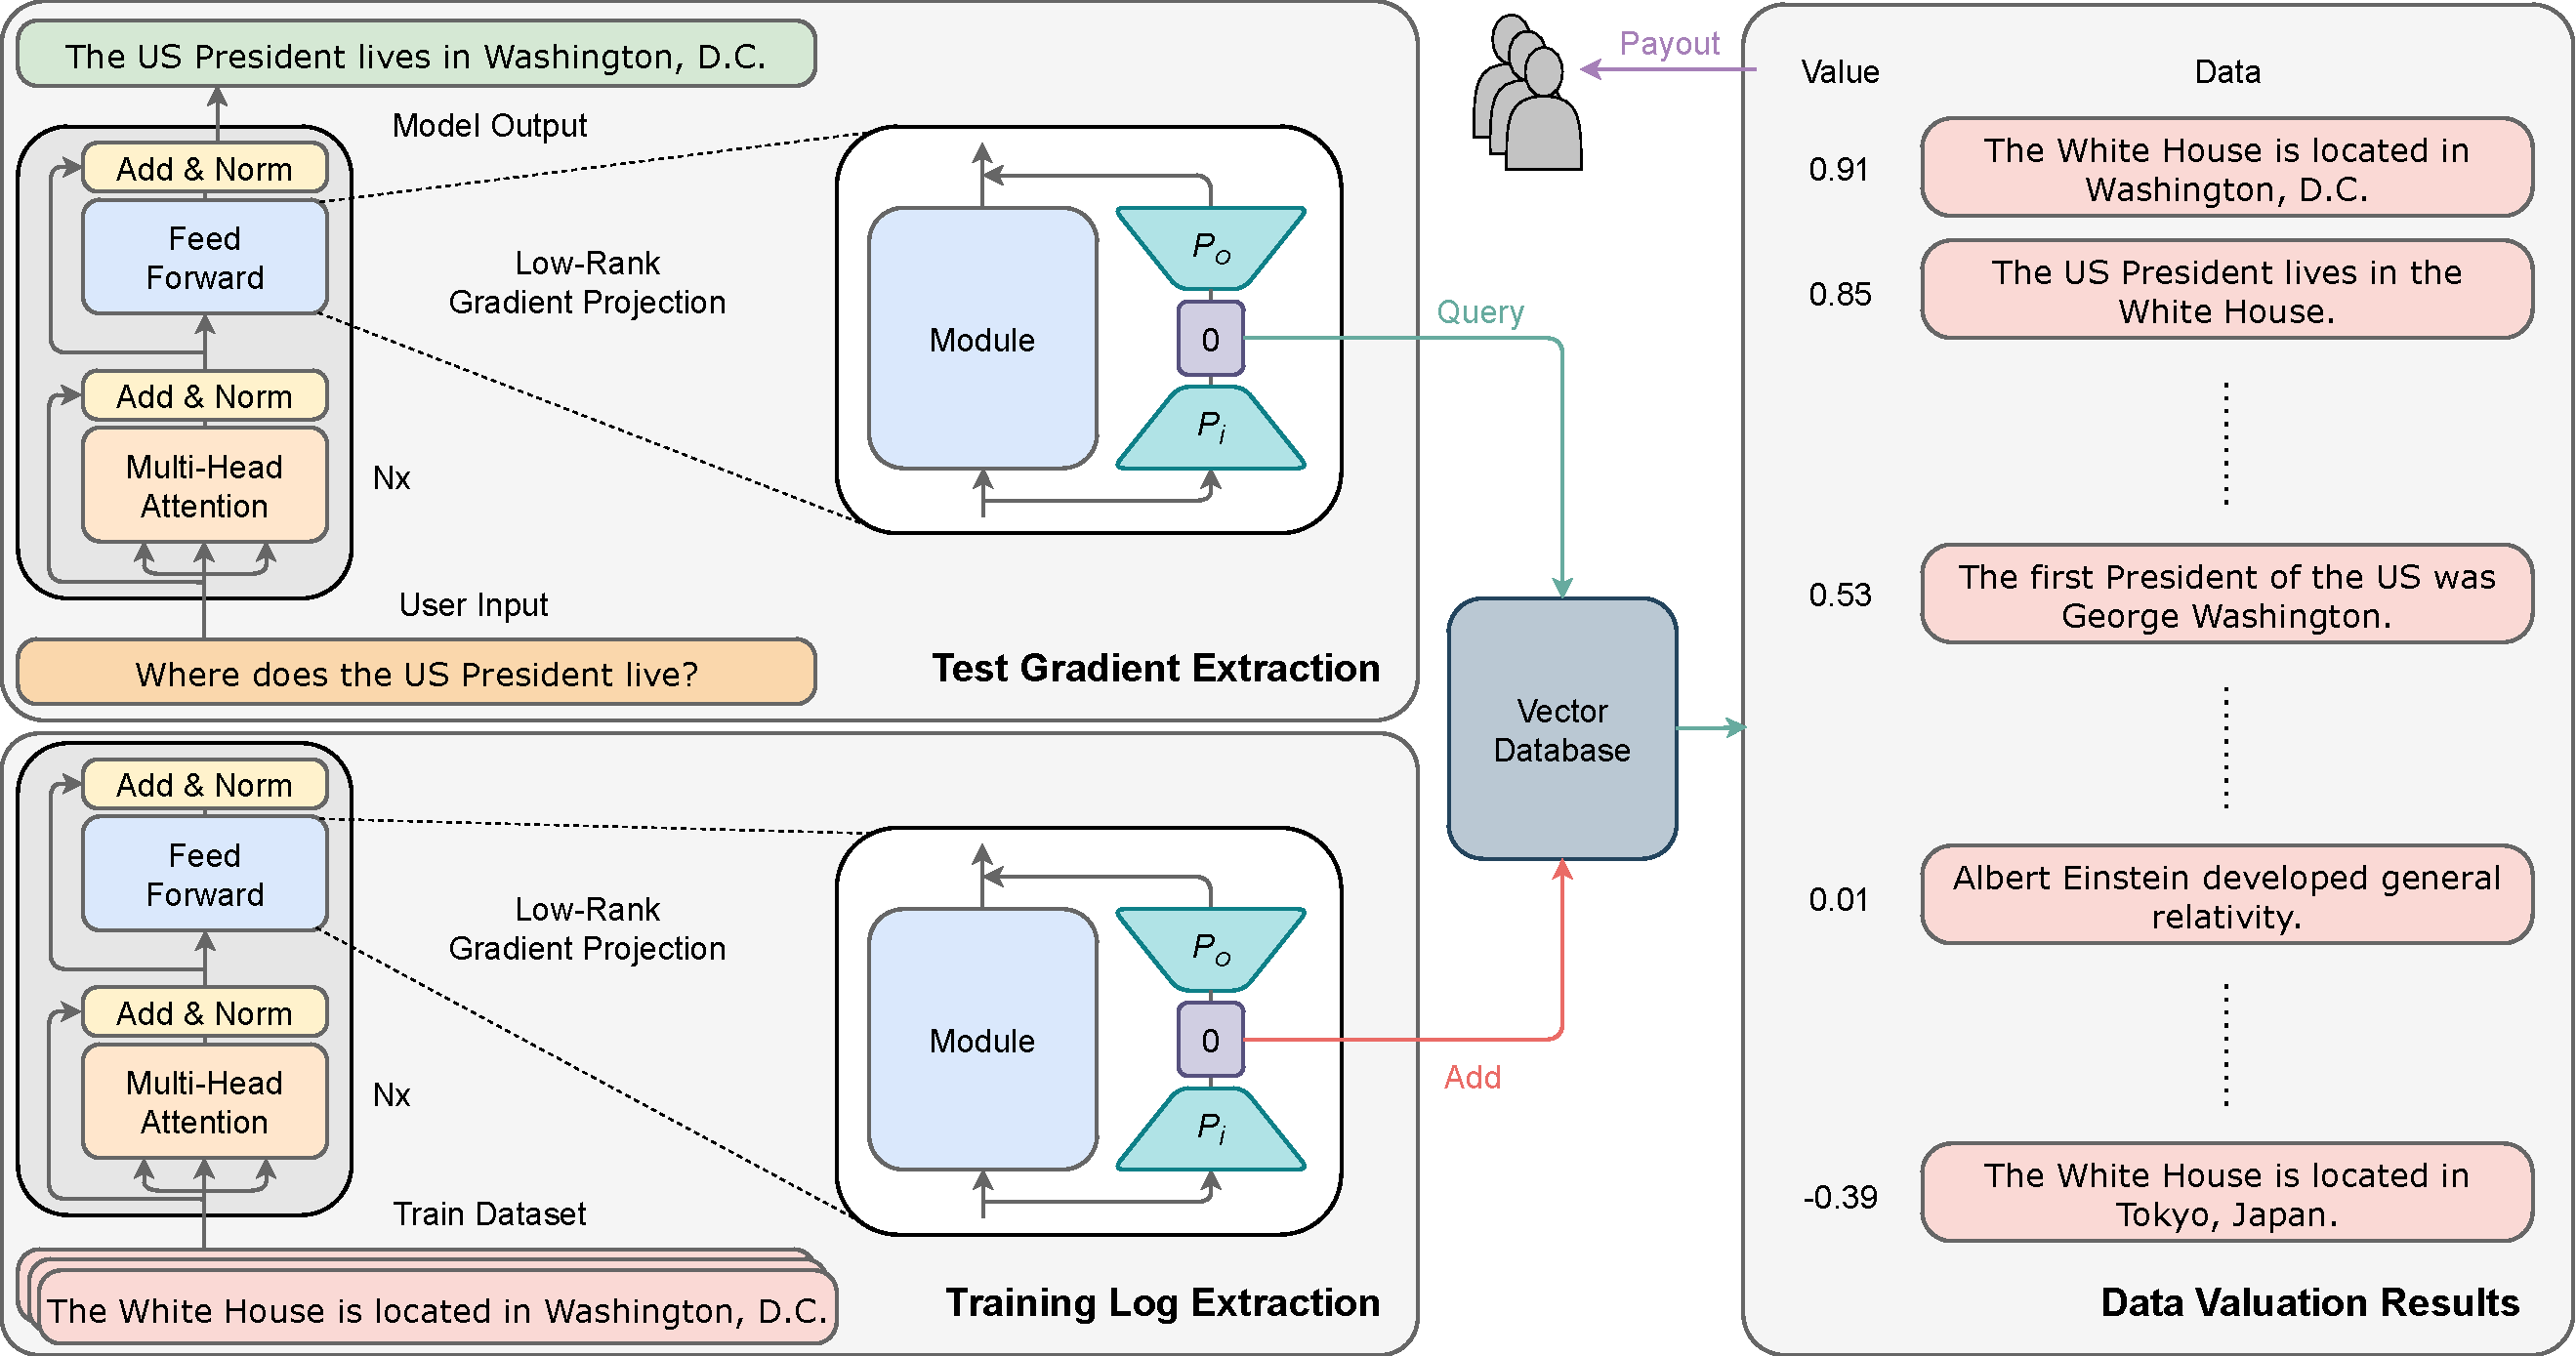
\includegraphics[width=0.94\textwidth]{figures/diagram_v7.pdf}
    \vskip -4pt
    \caption{Data valuation system architecture. \textbf{(Left Bottom)} We first extract the Hessian and gradients for all training data using efficient gradient projection \method\ and store them in a database. \textbf{(Left Top)} At test time, we similarly extract gradients and query the database. \textbf{(Right)} The database returns similarity scores with respect to training examples that can be used for data valuation/attribution.}
    \label{fig:diagram}
\end{figure}

\begin{itemize}[leftmargin=*,topsep=-2pt]
    \item Employing gradient structures in backpropagation, we develop a novel \textbf{lo}w-rank \textbf{gra}dient projection algorithm \method\ that improves space \& time complexity of gradient projection, a major scalability bottleneck in prior work~\cite{park2023trak,schioppa2022scaling}, from $O(nk)$ to $O(\sqrt{nk})$ where $n$ and $k$ are model and projection dimensions. Furthermore, \method\ directly computes projected gradients without materializing full gradients, enabling low GPU memory and high GPU utilization for improved efficiency. Lastly, we show that \method\ can be easily implemented with small add-on layers, similarly to LoRA~\cite{hu2021lora}.
    \item By interpreting a damping term in influence functions as a spectral gradient sparsification mechanism, we (1) offer a theoretical motivation of gradient projection approaches to influence functions and (2) derive a specialized PCA initialization scheme for \method.
    \item We introduce software named \software\ that (1) makes it \textit{simple} to convert existing training code into data valuation code, (2) is \textit{compatible} with various scalability tools and features in the LLM ecosystem, and (3) is \textit{extensible} to implement other data valuation or interpretability algorithms.
    \item In our data valuation experiments, \method\ demonstrates competitive accuracy against more costly baselines, while showing up to 6,500$\times$ increase in throughput and 5$\times$ reduction in GPU memory, when applied to Llama3-8B-Instruct~\cite{llama3modelcard} and the 1B-token dataset, compared to EKFAC influence \cite{grosse2023studying}, the state-of-the-art and only runnable baseline at this scale. We also observe that most valuable data identified by \method\ generally share qualitative similarities with the queried LLM output.
\end{itemize}

\section{Regularization of Deep Neural Networks}
\label{sec:kernel_reg}
%!TEX root = main.tex

In this section, we recall the kernel perspective on deep networks introduced
by~\citet{bietti2018group}, and present upper and lower bounds on the RKHS norm
of a given model, leading to various regularization strategies.  For
simplicity, we first consider real-valued networks and binary classification,
before discussing multi-class extensions.

\subsection{Relation between deep networks and RKHSs}
\label{sub:rkhs_construction}
Kernel methods consist of mapping data living in a set~$\Xcal$ to a
RKHS~$\Hcal$ associated to a positive definite kernel~$K$ through a mapping
function $\Phi: \Xcal \to \Hcal$, and then learning simple machine learning
models in~$\Hcal$. Specifically, when considering a real-valued regression or
binary classification problem, classical kernel methods find a prediction
function $f : \mathcal{X} \to \R$ living in the RKHS which can be written in linear
form, i.e., such that $f(x) = \langle f, \Phi(x) \rangle_\Hc$ for all~$x$
in~$\Xcal$.  While explicit mapping to a possibly infinite-dimensional space is
of course only an abstract mathematical operation, learning~$f$ can be done
implicitly by computing kernel evaluations and typically by using convex
programming~\citep{scholkopf2001learning}.

Moreover, the RKHS norm~$\|f\|_\Hc$ acts as a natural regularization function,
which controls the variations of model predictions
according to the geometry induced by~$\Phi$:
\begin{equation}
\label{eq:cs}
|f(x) - f(x')| \leq \|f\|_\Hc \cdot \|\Phi(x) - \Phi(x') \|_\Hc.
\end{equation}
Unfortunately, our setup does not allow us to use the RKHS norm in a traditional way since evaluating the kernel is intractable. Instead, we
propose a different approach that considers explicit parameterized
representations of functions contained in the RKHS, given by generic CNNs,
and leverage properties of the RKHS and the
kernel mapping in order to regularize when learning the network parameters.


Consider indeed a real-valued deep convolutional network $f : \mathcal{X} \to
\R$, where $\mathcal X$ is simply $\R^d$, with rectified linear unit (ReLU) activations and no bias units.
By constructing an appropriate multi-layer hierarchical kernel, \citet{bietti2018group} show
that the corresponding RKHS~$\Hc$ contains a CNN with the same architecture and parameters as~$f$,
but with activations that are smooth approximations of ReLU.
Although the model predictions might not be strictly equal, we will abuse notation and denote this
approximation with smooth ReLU by~$f$ as well,
with the hope that the regularization procedures derived from the RKHS model
will be effective in practice on the original CNN~$f$.

Besides, the mapping~$\Phi(\cdot)$ is shown to be non-expansive:
\begin{equation}
\label{eq:non_expansive}
\|\Phi(x) - \Phi(x') \|_\Hc \leq \|x - x'\|_2,
\end{equation}
so that controlling~$\|f\|_\Hc$ provides some robustness to additive $\ell_2$-perturbations, by~\eqref{eq:cs}.
Additionally, with appropriate pooling operations, \citet{bietti2018group} show that the kernel mapping is also
stable to deformations, meaning that the RKHS norm also controls robustness to translations
and other transformations including scaling and rotations,
which can be seen as deformations when they are small.

In contrast to standard kernel methods, where the RKHS norm is typically available in closed form, this norm is difficult to compute in our setup, and requires approximations.
The following sections present upper and lower bounds on~$\|f\|_{\Hcal}$,
with linear convolutional operations denoted by~$W_k$ for $k=1, \ldots, L$, where~$L$ is the number of layers.
Defining~$\theta := \{W_k : k = 1, \ldots, L\}$, we then leverage these bounds to approximately solve the following
penalized or constrained optimization problems on a training set~$(x_i, y_i), i = 1, \ldots, n$:
\begin{align}
\label{eq:penalty_or_constraint}
& \min_\theta \frac{1}{n} \sum_{i=1}^n \ell(y_i, f_\theta(x_i)) + \lambda \|f_\theta\|_\Hc^2 \quad \text{or } \\
& \min_{\theta: \|f_\theta\|_\Hc \leq C} \frac{1}{n} \sum_{i=1}^n \ell(y_i, f_\theta(x_i)).
\end{align}
We also note that while the construction of~\citet{bietti2018group} considers VGG-like networks~\citep{simonyan2014very},
the regularization algorithms we obtain in practice can be easily adapted to different architectures
such as residual networks~\citep{he2016deep}.

\subsection{Exploiting lower bounds of the RKHS norm}
\label{sub:lower_bounds}

In this section, we devise regularization algorithms by leveraging lower bounds on~$\|f\|_\Hc$,
obtained by relying on the following variational characterization of Hilbert norms:
\begin{equation*}
\|f\|_\Hc = \sup_{\|u\|_\Hc \leq 1} \langle f, u \rangle_\Hc.
\end{equation*}
At first sight, this definition is not useful since the set $U = \{u \in \Hc : \|u\|_\Hc \leq 1\}$ may be 
infinite-dimensional
 and the inner products $\langle f, u \rangle_\Hc$ cannot be
computed in general. Thus, we devise tractable lower bound approximations by considering smaller sets~$\bar{U} \subset U$.

\paragraph{Adversarial perturbation penalty.}
Thanks to the non-expansiveness of $\Phi$, we can consider the subset $\bar U \subset U$ defined as $\bar{U} = \{\Phi(x + \delta) - \Phi(x) : x \in \mathcal X, \|\delta\|_2 \leq 1 \}$,
leading to the bound
\begin{equation}
\label{eq:lower_bound}
\|f\|_\Hc  \geq  \|f\|_\delta^2 := \sup_{x \in \mathcal X, \|\delta\|_2 \leq 1} f(x + \delta) - f(x),
\end{equation}
which is reminiscent of adversarial perturbations. Adding a regularization parameter $\epsilon > 0$ in front of the norm
then corresponds to different sizes of perturbations:
\begin{equation}
\label{eq:kernel_adv}
\epsilon \|f\|_\Hc = \sup_{\|u\|_\Hc \leq \epsilon} \langle f, u \rangle_\Hc \geq \sup_{x \in \mathcal X, \|\delta\|_2 \leq \epsilon} f(x + \delta) - f(x).
\end{equation}
Using this lower bound or its square as a penalty in the objective~\eqref{eq:penalty_or_constraint}
when training a CNN provides a way to regularize.
Optimizing over adversarial perturbations has been useful to obtain robust models~\citep[\eg, the PGD method of~][]{madry2018towards};
yet our approach differs in two important ways: 

(i) it involves a penalty that is decoupled from the loss term such that 
in principle, our penalty could be used beyond the supervised empirical risk paradigm.
In contrast, PGD optimizes the robust formulation~\eqref{eq:robust} below, which 
fits training data while considering
perturbations on the loss.

(ii) our penalty involves a global maximization problem
on the input space~$\Xcal$, as opposed to only maximizing on perturbations near
training data. In practice, optimizing over~$\Xcal$ is however
difficult and instead, we replace~$\Xcal$ by random mini-batches of examples,
yielding further lower bounds on the RKHS norm. These examples may be labeled or not,
in contrast to PGD that perturb labeled examples only.
When using such a mini-batch,
a gradient of the penalty can be obtained by first finding maximizers~$\hat x, \hat \delta$
(where~$\hat x$ is an element of the mini-batch and $\hat{\delta}$ is a perturbation), and then computing gradients
of $f_\theta(\hat x + \hat \delta) - f_\theta(\hat x)$ with respect to~$\theta$ by using back-propagation.
In practice, we compute the perturbations~$\delta$ for each example~$x$ by using a few steps of
projected gradient ascent with constant step-lengths.

\paragraph{Robust optimization yields another lower bound.}
In some contexts, our penalized approach is related to solving the robust optimization problem
\begin{equation}
\label{eq:robust}
\min_\theta \frac{1}{n} \sum_{i=1}^n \sup_{\|\delta\|_2 \leq \epsilon} \ell(y_i, f_\theta(x_i + \delta)),
\end{equation}
which is commonly considered for training adversarially robust classifiers~\citep{wong2018provable,madry2018towards,raghunathan2018certified}.
In particular, \citet{xu2009robustness} show that the penalized and
robust objectives are equivalent in the case of the hinge loss with linear predictors,
when the data is non-separable.
They also show the equivalence for kernel methods when considering the (intractable) full perturbation set~$U$
around each point in the RKHS~$\Phi(x_i)$, that is, predictions $\langle f, \Phi(x_i) + u \rangle_\Hc$ with~$u$ in $U$.
Intuitively, when a training example $(x_i, y_i)$ is misclassified, we are in the ``linear'' part of the hinge loss, such~that
\begin{equation*}
\sup_{\|u\|_\Hc \leq \epsilon} \ell(y_i, \langle f, \Phi(x_i) + u \rangle_\Hc) = \ell(y_i, f(x_i)) + \epsilon \|f\|_{\Hcal}.
\end{equation*}
For other losses such as the logistic loss, a regularization effect is still present even
for correctly classified examples,
though it may be smaller since the loss has a reduced slope for such points.
This leads to an \emph{adaptive} regularization mechanism that may automatically reduce
the amount of regularization when the data is easily separable.
However, the robust optimization approach might only encourage local stability around training examples, while the global quantity~$\|f\|_\Hc$
may become large in order to better fit the data.
We note that a perfect fit of the data with large complexity does not prevent generalization~\citep[see, \eg,][]{belkin2018overfitting,belkin2018understand};
yet, such mechanisms are still poorly understood.
Nevertheless, it is easy to show that the robust objective~\eqref{eq:robust}
lower bounds the penalized objective with penalty~$\epsilon \|f\|_{\Hcal}$.

\paragraph{Gradient penalties.}
Taking $\bar{U} \!= \! \{\frac{\Phi(x) - \Phi(y)}{\|x - y\|_2} : x, y \!\in\! \mathcal X\}$, which is a subset of~$U$
by Eq.~\eqref{eq:non_expansive}---it turns out that this is the same set as for adversarial perturbation penalties,
since~$\Phi$ is homogeneous~\citep{bietti2018group} and $\mathcal X =
\Real^d$---we obtain a lower bound based on the Lipschitz constant of~$f$:
\begin{equation}
\|f\|_\Hc \geq \sup_{x, y \in \mathcal{X}} \frac{f(x) - f(y)}{\|x - y\|_2} \geq \|\nabla f\| := \sup_{x \in \mathcal X} \|\nabla f(x)\|_2, \label{eq:gradientpenalty}
\end{equation}
where the second inequality becomes an equality when~$\Xcal$ is convex,
and the supremum is taken over points where~$f$ is differentiable.
Although we are unaware of previous work using this exact lower bound for a generic regularization penalty,
we note that variants replacing the supremum over~$x$ by an expectation over data have been recently used
to stabilize the training of generative adversarial networks~\citep{gulrajani2017improved,roth2017stabilizing},
and we provide insights in Section~\ref{sub:gan_reg} on the benefits of RKHS regularization in such a setting.
Related penalties have been considered in the context of robust optimization,
for regularization or robustness,
noting that a penalty based on the gradient of the loss function $x \mapsto \ell(y, f(x))$ can give a good approximation of~$\eqref{eq:robust}$
when~$\epsilon$ is small~\citep{drucker1991double,lyu2015unified,roth2018adversarially,simon2018adversarial}.

\paragraph{Penalties based on deformation stability.}
We may also obtain new penalties by considering more exotic sets
$\bar{U} = \{\Phi(\tilde x) - \Phi(x) : x~\in~{\mathcal X},~ \tilde x \text{ is a small} \text{ deformation of }x\}$,
where the amount of deformation is dictated by the stability bounds of~\citet{bietti2018group} in order to ensure that $\bar{U} \subset U$.
More precisely, such bounds depend on the maximum displacement and Jacobian norm of
the diffeomorphisms considered. These can be easily computed for various parameterized families
of transformations, such as translations, scaling or rotations, leading to simple ways to control
the regularization strength through the parameters of these transformations.
One can also consider infinitesimal deformations from such parameterized transformations,
which approximately yields the \emph{tangent propagation} regularization
strategy of~\citet{simard1998transformation}.
These approaches are detailed in Appendix~\ref{sec:deformation_penalties}.
If instead we consider the robust optimization formulation~\eqref{eq:robust}, we obtain a form
of \emph{data augmentation} where transformations are optimized instead of sampled, as done by~\citep{engstrom2017rotation}.


\paragraph{Extensions to multiple classes and beyond}
\label{sub:multiclass}

We now extend the regularization strategies based on lower bounds to multi-valued networks,
in order to deal with multiple classes.
For that purpose, we consider a multi-class penalty $\|f_1\|_\Hc^2 + \ldots + \|f_K\|_\Hc^2$
for an~$\R^K$-valued function $f = (f_1, f_2, \ldots, f_K)$, and we define 
\begin{align*}
\|f\|_\delta^2 := \sum_{k=1}^K \|f_k\|_\delta^2 \text{~~~and~~~} \|\nabla f\|^2 := \sum_{k=1}^K \|\nabla f_k\|^2,
\end{align*}
where $\|f_k\|_\delta$ is the adversarial penalty~(\ref{eq:lower_bound}), and $\|\nabla f_k\|$ is defined in~(\ref{eq:gradientpenalty}).
For deformation stability penalties, we proceed in a similar manner,
and for robust optimization formulations~\eqref{eq:robust}, the extension is straightforward,
given that multi-class losses such as cross-entropy can be
directly optimized in an adversarial training or gradient penalty setup.

Finally, we note that while the kernel approach we introduce considers
the Euclidian geometry in the input space, it is possible to consider heuristic alternatives for other
geometries, such as~$\ell_\infty$ perturbations, as discussed in Appendix~\ref{sec:non_euclidian_appx}.

\subsection{Exploiting upper bounds with spectral norms}
\label{sub:upper_bounds}

Instead of lower bounds, one may use instead
 the following upper bound from~\citet[Proposition 14]{bietti2018group}:
\begin{equation}
\label{eq:upper_bound}
\|f\|_\Hc \leq \omega(\|W_1\|, \ldots, \|W_L\|),
\end{equation}
where~$\omega$ is increasing in all of its arguments, and~$\|W_k\|$ is the spectral norm of the linear
operator~$W_k$.
Here, we simply consider the spectral norm on the filters, given by~$\|W\| := \sup_{\|x\|_2 \leq 1} \|W x\|_2$.
Other generalization bounds relying on similar quantities have been proposed for
controlling complexity~\citep{bartlett2017spectrally,neyshabur2017pac}, suggesting that using them for
regularization is relevant even beyond our kernel perspective,
as observed by~\citet{cisse2017parseval,sedghi2018singular,yoshida2017spectral}.
Extensions to multiple classes are simple to obtain by simply considering spectral norms up to
the last layer.


\paragraph{Penalizing the spectral norms.}
One way to control the upper bound~\eqref{eq:upper_bound} when learning a neural network~$f_\theta$
is to consider a regularization penalty based on spectral norms
\begin{equation} 
	\label{eq:optimization_problem_penalized} 
	\min_{\theta}\frac{1}{n} \sum_{i=1}^{n} \ell(y_i, f_{\theta}(x_i)) + \lambda \sum_{l=1}^{L} \|W_l\|^2,
\end{equation}
where~$\lambda$ is a regularization parameter.
To optimize this cost, one can obtain (sub)gradients of the penalty by computing singular vectors
associated to the largest singular value of each~$W_l$.
We consider the method of~\citet{yoshida2017spectral}, which computes such singular vectors approximately
using one or two iterations of the power method, as well as a more costly approach using the full SVD.

\paragraph{Constraining the spectral norms with a continuation approach.}
In the constrained setting, we want to optimize:
\begin{equation*}
\begin{aligned}
\min_{\theta}\frac{1}{n} \sum_{i=1}^{n} \ell(y_i, f_{\theta}(x_i)) \text{~~s.t.~~} \|W_l\| \leq \tau \text{ ; } l\in 1, \dots, L~,
\end{aligned}
\end{equation*}
where $\tau$ is a user-defined constraint.
This objective may be optimized by projecting each~$W_l$ in the
spectral norm ball of radius $\tau$ after each gradient step.
Such a projection is achieved by truncating the singular values to be smaller than~$\tau$ (see Appendix~\ref{sec:spectral_norms_appx}).
We found that the loss was hardly optimized with this approach,
and therefore introduce a continuation approach with an exponentially
decaying schedule for~$\tau$ reaching a constant $\tau_0$
after a few epochs, which we found to be important for good empirical performance.

\subsection{Combining upper and lower bounds.}
One advantage of lower bound penalties is that they are independent of
the model parameterization, making them flexible enough to use with more complex architectures.
In addition, the connection with robust optimization can provide a useful mechanism for adaptive regularization.
However, they do not provide a guaranteed control on the RKHS norm, unlike the upper bound strategies.
This is particularly true for robust optimization approaches, which may favor small training loss
and local stability over global stability through~$\|f\|_\Hc$.
Nevertheless, we observed that our new approaches based on separate penalties
sometimes do help in controlling upper bounds as well (see Section~\ref{sec:experiments}).

While these upper bound strategies are useful for limiting model complexity,
we found them empirically less effective for robustness (see Section~\ref{sub:exp_robust}).
However, we observed that combining with lower bound approaches can overcome this weakness,
perhaps due to a better control of local stability.
In particular, such combined approaches often provide the best generalization performance
in small data scenarios, as well as better guarantees on adversarially robust generalization
thanks to a tighter control of the RKHS norm.



\section{Theoretical Guarantees and Insights}
\label{sec:theory}
%!TEX root = main.tex

In this section, we study how the kernel perspective allows us to extend standard margin-based generalization bounds 
to an adversarial setting in order to
provide theoretical guarantees on adversarially robust generalization.
We then discuss how our kernel approach provides novel interpretations for training
generative adversarial networks.

\subsection{Guarantees on adversarial generalization}
\label{sub:guarantees}

While various methods have been introduced to empirically gain robustness to adversarial perturbations,
the ability to generalize with such perturbations, also known as \emph{adversarial generalization}~\citep{schmidt2018adversarially},
still lacks theoretical understanding.
Margin-based bounds have been useful
to explain the generalization behavior of learning algorithms that can fit the training data
well, such as kernel methods, boosting and neural networks~\citep{koltchinskii2002empirical,boucheron2005theory,bartlett2017spectrally}.
Here, we show how such arguments can be adapted to obtain guarantees on adversarial generalization,
\ie, on the expected classification error in the presence of an~$\ell_2$-bounded adversary,
based on the RKHS norm of a learned model.
For a binary classification task with labels in $\mathcal Y = \{-1,1\}$ and data distribution~$\mathcal D$,
we would like to bound the expected adversarial error of a classifier~$f$, given for some $\epsilon > 0$ by
\begin{equation}
\label{eq:adv_error}
\text{err}_\mathcal D(f, \epsilon) := P_{(x,y) \sim \mathcal D} (\exists \|\delta\|_2 \leq \epsilon: ~y f(x + \delta) < 0).
\end{equation}
Leveraging the fact that~$f$ is $\|f\|_\Hc$-Lipschitz,
we now show how to further bound this quantity using empirical margins,
following the usual approach to obtaining margin bounds for kernel methods~\citep[\eg,][]{boucheron2005theory}.
Consider a training dataset $(x_1, y_1), \ldots, (x_n, y_n) \in \mathcal X \times \mathcal Y$.
Defining $L_n^\gamma(f) := \frac{1}{n} \sum_{i=1}^n \textbf{1}\{y_i f(x_i) < \gamma\}$,
we have the following bound, proved in Appendix~\ref{sec:generalization_appx}:
\begin{proposition}[Adversarially robust margin bound]
\label{prop:robust_margin_bound}
With probability~$1 - \delta$ over a dataset $\{(x_i, y_i)\}_{i=1, \ldots, n}$, we have,
for all choices of $\gamma > 0$ and~$f \in \Hc$,
\begin{align}
\label{eq:robust_margin_bound}
& \text{err}_\mathcal D(f, \epsilon) \leq L_n^{\gamma + 2 \epsilon \|f\|_\Hc}(f) + \tilde{O}\left( \frac{\|f\|_\Hc \bar{B}}{\gamma \sqrt{n}}  \right),
\end{align}
where $\bar{B} = \sqrt{\frac{1}{n}\sum_{i=1}^n K(x_i, x_i)}$ and $\tilde{O}$ hides a term depending logarithmically on~$\|f\|_\Hc, \gamma$, and $\delta$.
\end{proposition}

When $\epsilon = 0$, we obtain the usual margin bound, while $\epsilon > 0$ yields
a bound on adversarial error~$\text{err}_\mathcal D(f, \epsilon)$,
for some neural network~$f$ learned from data.
Note that other complexity measures based on products of spectral norms may be used instead of~$\|f\|_\Hcal$,
as well as multi-class extensions, following~\citet{bartlett2017spectrally,neyshabur2017pac}.
In concurrent work, \citet{khim2018adversarial,yin2019rademacher} derive similar bounds
in the context of fully-connected networks.
In contrast to these works, which bound complexity of a modified function class,
our bound uses the complexity of the original class and leverages smoothness properties
of functions to derive the margin bound.

One can then study the effectiveness of a regularization algorithm by inspecting
cumulative distribution (CDF) plots of the
\emph{normalized margins} $\bar{\gamma}_i = y_i f(x_i) / \|f\|_\Hc$,
for different strengths of regularization (an example is given in Figure~\ref{fig:norms_and_margins}, Section~\ref{sub:exp_robust}).
According to the bound~\eqref{eq:robust_margin_bound}, one can assess expected adversarial error with $\epsilon$-bounded perturbations
by looking at the part of the plot to the right of~$\bar{\gamma} = 2\epsilon$.
In particular, the value of the CDF at such a value of~$\bar{\gamma}$ is representative of the
bound for large~$n$ (since the second term is negligible),
while for smaller~$n$, the best bound is obtained for a larger value of~$\bar{\gamma}$, which also suggests that
the right side of the plots is indicative of performance on small datasets.

When the RKHS norm can be well approximated, our bound provides a certificate on
test error in the presence of adversaries. 
While such an approximation is difficult to
obtain in general, the guarantee is most useful when lower and upper bounds of the RKHS norm are controlled together.


\subsection{New insights on generative adversarial networks}
\label{sub:gan_reg}

Generative adversarial networks (GANs) attempt to learn a \emph{generator} neural network~$G_\phi : \mathcal Z \to \mathcal X$,
so that the distribution of~$G_\phi(z)$ with~$z \sim D_z$ a noise vector resembles a data distribution~$D_x$.
In this section, we discuss connections between recent regularization techniques for
training GANs, and approaches to learning generative models
based on a MMD criterion~\citep{gretton2012kernel}, in view of our RKHS framework.
Our goal is to provide a new insight on these methods, but not necessarily to provide a new one.

Various recent approaches have relied on regularization strategies on a \emph{discriminator} network
in order to improve the stability of GAN training and the quality of the produced samples.
Some of these resemble the approaches presented in Section~\ref{sec:kernel_reg}
such as gradient penalties~\citep{gulrajani2017improved,roth2017stabilizing}
and spectral norm regularization~\citep[]{miyato2018spectral}.
We provide an RKHS interpretation of these methods as
optimizing an MMD distance with the convolutional kernel introduced in Section~\ref{sec:kernel_reg}:
\begin{equation}
\label{eq:ckn_mmd}
\min_\phi \sup_{\|f\|_\Hc \leq 1} \E_{x \sim D_x}[ f(x)] - \E_{z \sim D_z}[f(G_\phi(z))].
\end{equation}
When learning from an empirical distribution over~$n$ samples,
the MMD criterion is known to have much better sample complexity than the Wasserstein-1
distance considered by~\citet{arjovsky2017wasserstein} for high-dimensional data
such as images~\citep{sriperumbudur2012empirical}.
While the MMD approach has been used for training generative models, it generally relies on a generic kernel function,
such as a Gaussian kernel, that appears explicitly in the objective~\citep{dziugaite2015training,li2017mmd,binkowski2018demystifying}.
Although using a learned feature extractor can improve this, the Gaussian kernel might be a poor choice when
dealing with natural signals such as images, while the hierarchical kernel we consider in our paper is better suited
for this type of data, by providing useful invariance and stability properties.
Leveraging the variational form of the MMD~\eqref{eq:ckn_mmd} with this kernel suggests for instance using convolutional networks
as the discriminator~$f$, with constraints on the spectral norms in order to ensure~$\|f\|_\Hc \leq C$ for some~$C$,
as done by~\citet{miyato2018spectral} through normalization.


\section{Experiments}
\label{sec:experiments}
\section{Experiments}
\label{sec:experiments}

We validate our approach empirically, showing that our Monarch matrix parametrization achieves a favorable efficiency--accuracy tradeoff compared to baselines on a wide range of domains (text, images, PDEs, MRI), in three settings (E2E training, S2D training, and D2S fine-tuning):
\begin{itemize}[leftmargin=*,nosep,nolistsep,noitemsep]
\item
In \cref{subsec:benchmark_tasks}, on image classification and language modeling benchmarks, such as ViT / MLP Mixer on ImageNet and GPT-2 on Wikitext-103, Monarch is 2$\times$ faster to train than dense models, while achieving the same accuracy / perplexity. In \cref{subsec:pde_mri}, in scientific and medical domains where special transforms (Fourier) are common, Monarch outperforms Fourier transform based methods on PDE solving, with up to 40\% lower error, and on MRI reconstruction attains up to 15\% higher pSNR and 3.8\% higher SSIM.
\item In \cref{subsec:pde_mri}, we show that on the large OpenWebText dataset, reverse sparsification (training with Monarch weight matrices for most of the time, then transitioning to dense weight matrices) speeds up the pretraining of GPT-2 models by 2$\times$ compared to the dense model, with no loss in upstream or downstream quality.
Moreover, reverse sparsification speeds up BERT pretraining by 23\% even compared to the implementation from Nvidia that set the MLPerf~\citep{mattson2020mlperf} 1.1 record.
\item In \cref{subsec:finetuning}, as a proof of concept, we demonstrate that our Monarch approximation algorithm can improve fine-tuning efficiency for pretrained models. We show that compressing BERT to a Monarch matrix model performs comparably to a finetuned dense model on GLUE, with 2$\times$ fewer parameters and 1.7$\times$ faster finetuning speed.
\end{itemize}

\subsection{End-to-End Training}
\label{subsec:e2e_training}
\subsubsection{Benchmark Tasks: Image Classification, Language Modeling}
\label{subsec:benchmark_tasks}

We show that replacing dense matrices with Monarch matrices in ViT, MLP-Mixer, and
GPT-2 can speed up training by up to 2$\times$ without sacrificing model quality in~\cref{table:pretrain,table:gpt_pretrain}.

\textbf{Setup.} We use the popular vision benchmark, ImageNet~\citep{deng2009imagenet}. We choose recent popular Vision Transformer~\citep{dosovitskiy2020image}, and MLP-Mixer~\citep{tolstikhin2021mlp} as representative base dense models.
For language modeling, we evaluate GPT-2~\citep{radford2019language} on WikiText-103~\citep{merity2016pointer}.

\begin{table}[h]
  \small
  \centering
  \vspace{-2mm}
  \caption{\label{table:pretrain}The performance of Monarch matrices and ViT / MLP-Mixer on ImageNet, including the number of parameters and FLOPs. We measure the Top-1 accuracy and the training time speedup compared to the corresponding dense model. %
  \vspace{2mm}
  }
  \iftoggle{arxiv}{}{
  \resizebox{\linewidth}{!}
  }
  {
  \setlength{\tabcolsep}{3pt}
  \vspace{3em}
  \begin{tabular}{@{}c||ccccccc@{}}
  \specialrule{.15em}{.05em}{.05em}
    Model&\multicolumn{1}{c}{ImageNet acc.}&\multicolumn{1}{c}{Speedup} &\multicolumn{1}{c}{Params} & \multicolumn{1}{c}{FLOPs} \\
    \specialrule{.15em}{.05em}{.05em}
    Mixer-S/16& 74.0& - & 18.5M & 3.8G \\
    Monarch-Mixer-S/16& 73.7& 1.7$\times$ & 7.0M & 1.5G \\
    Mixer-B/16& 77.7& - & 59.9M & 12.6G \\
    Monarch-Mixer-B/16& 77.8& 1.9$\times$ & 20.9M & 5.0G \\
    \specialrule{.15em}{.05em}{.05em}
    ViT-S/16& 79.4 & - & 48.8M & 9.9G \\
    Monarch-ViT-S/16& 79.1 & 1.9$\times$ & 19.6M & 3.9G \\
    ViT-B/16& 78.5 & - & 86.6M  & 17.6G \\
    Monarch-ViT-B/16& 78.9 & 2.0$\times$ & 33.0M & 5.9G \\
    \specialrule{.15em}{.05em}{.05em}
  \end{tabular}
  }
\end{table}

\begin{table}[h]
  \small
  \centering
  \vspace{-3mm}
  \caption{\label{table:gpt_pretrain} Performance of Monarch matrices and GPT-2-Small/Medium on WikiText-103, including the \# of parameters and FLOPs. Monarch achieves similar perplexity (ppl) but 2.0$\times$ faster.}
  \vspace{1mm}
  \iftoggle{arxiv}{}{
    \resizebox{0.95\linewidth}{!}
  }
  {
\setlength{\tabcolsep}{5pt}
\begin{tabular}{c||cccc}
\specialrule{.15em}{.05em}{.05em}
\multirow{1}{*}{{ Model} } & \multicolumn{1}{c}{\multirow{1}{*}{PPL}}
                              & \multicolumn{1}{c}{\multirow{1}{*}{Speedup}}
                              & \multicolumn{1}{c}{\multirow{1}{*}{Params}}
                              & \multicolumn{1}{c}{\multirow{1}{*}{FLOPs}}\\
\specialrule{.15em}{.05em}{.05em}
GPT-2-Small &  20.6 & - & 124M& 106G\\
Monarch-GPT-2-Small& 20.7  & 1.8$\times$ &72M & 51G\\
\specialrule{.15em}{.05em}{.05em}
GPT-2-Medium &  20.9 & - & 355M& 361G\\
Monarch-GPT-2-Medium& 20.3  & 2.0$\times$ &165M & 166G\\
\specialrule{.15em}{.05em}{.05em}
\end{tabular}
}
\vspace{-2mm}
\end{table}


\subsubsection{PDE solving and multi-coil MRI reconstruction}
\label{subsec:pde_mri}

Many scientific or medical imaging tasks rely on specialized transforms such as the
Fourier transform.
We show that replacing the fixed Fourier transform with the more expressive
Monarch matrices yields higher model quality (lower reconstruction error) with
comparable model speed.

\textbf{Solving PDEs with Monarch Neural Operators.}
We follow the experimental setting in FNO~\citep{li2020fourier} and apply a Monarch--based neural operator to the task of solving the Navier--Stokes PDE. Compared to baseline U-Nets~\citep{ronneberger2015u}, TF-Nets~\citep{wang2020towards}, ResNets~\citep{he2016deep} and FNOs~\cite{li2020fourier}, neural operators based on Monarch improve solution accuracy across spatial resolutions by up to $40\%$ (Table \ref{table:pde}).  





\paragraph{Non-periodic boundary conditions.} Traditional spectral methods based on Fourier transform work best with periodic boundary conditions and forcing terms. However, PDEs of practical interest often exhibit non--periodic or even unknown boundary conditions. Monarch operators are not constrained to the Fourier transform and can thus still learn the solution operator with excellent accuracy.

\begin{table}[h!] 
\scriptsize
\vspace{-4mm}
\caption{\label{table:pde}Benchmarks on Navier-Stokes (fixing resolution 64 × 64 for both training and testing).
Decreasing the viscosity coefficient $\nu$ makes the dynamics more chaotic.
}
\vspace{1mm}
\centering
\iftoggle{arxiv}{}{
  \resizebox{0.9\linewidth}{!}
}
{
\renewcommand{\arraystretch}{1}
\begin{tabular}{ c||ccc }
\specialrule{.15em}{.05em}{.05em}
Model & $v = 10^{-3}$  &  $v = 10^{-4}$ & $v = 10^{-5}$\\
\specialrule{.15em}{.05em}{.05em}
U-Net & 0.025  & 0.205  &   0.198\\
TF-Net  & 0.023  & 0.225 &  0.227 \\
ResNet & 0.070 &  0.287 &  0.275 \\
FNO & 0.017  & 0.178 & 0.155\\
Monarch-NO & \textbf{0.010} & \textbf{0.145} & \textbf{0.136} \\
\specialrule{.15em}{.05em}{.05em}
\end{tabular}
}
\textbf{\vspace{-3mm}}
\end{table}

\textbf{Accelerated MRI Reconstruction.} We characterize the utility of Monarch-based FFT operations for accelerated MRI reconstruction, a task which requires methods with both structured Fourier operators and dealiasing properties to recover high quality images. On the clinically-acquired 3D MRI SKM-TEA dataset \citep{desai2021skm}, Monarch-SENSE (mSENSE) enhances image quality by over 1.5dB pSNR and 2.5\% SSIM compared to zero-filled SENSE and up to 4.4dB and 3.8\% SSIM compared to U-Net baselines in data-limited settings. Setup details are available in~\cref{sec:experiment_details_mri}.

\paragraph{Expressive FFT.} By definition, standard IFFT in zero-filled SENSE cannot dealias the signal, resulting in artifacts in the reconstructed image. mSENSE replaces the inverse FFT (IFFT) operation in standard SENSE with learnable Monarch matrices. Thus, mSENSE preserves the structure of the Fourier transform while learning to reweight frequencies to suppress aliasing artifacts. Across multiple accelerations, mSENSE achieved up to +1.5dB and 2.5\% improvement in peak signal-to-noise ratio (pSNR) and structural similarity (SSIM), respectively (Table~\ref{table:mri}).

\paragraph{Data Efficiency.} While CNNs have shown promise for MRI reconstruction tasks, training these networks requires extensive amounts of labeled data to avoid overfitting. However, large data corpora are difficult to acquire in practice. mSENSE can be trained efficiently with limited supervised examples. In few shot settings, mSENSE can outperform U-Net by +4.4dB ($\approx$15\%) and 3.8\% SSIM (Table~\ref{table:mri-data-limited}). 







\begin{table}[h!] 
\scriptsize
\vspace{-3mm}
\caption{\label{table:mri}Mean $\pm$ standard error of the mean of conventional and Monarch-SENSE (mSENSE) on dual-echo (E1,E2) MRI reconstruction at multiple acceleration factors (Acc.).
}
\vspace{1mm}
\centering
\iftoggle{arxiv}{}{
  \resizebox{\linewidth}{!}
}
{
\renewcommand{\arraystretch}{1.2}
\begin{tabular}{c||ccccc}
\specialrule{.15em}{.05em}{.05em}
  & & \multicolumn{2}{c}{pSNR (dB) ($\uparrow$)} & \multicolumn{2}{c}{SSIM ($\uparrow$)} \\
  Acc. & Model &             E1 &             E2 &                E1 &                E2 \\
\specialrule{.15em}{.05em}{.05em}
\multirow{2}{*}{2} & SENSE &  32.8$\pm$0.2 &  35.4$\pm$0.2 &  0.871$\pm$0.003 &  0.865$\pm$0.003 \\
  & mSENSE &  \textbf{34.3$\pm$0.2} &  \textbf{36.6$\pm$0.2} &  \textbf{0.886$\pm$0.002} &  \textbf{0.882$\pm$0.003} \\
\specialrule{.15em}{.05em}{.05em}
\multirow{2}{*}{3} & SENSE &  30.9$\pm$0.2 &  33.5$\pm$0.2 &  0.819$\pm$0.004 &  0.795$\pm$0.004 \\
  & mSENSE &  \textbf{32.3$\pm$0.2} &  \textbf{34.6$\pm$0.2} &  \textbf{0.843$\pm$0.003} &  \textbf{0.820$\pm$0.004} \\
\specialrule{.15em}{.05em}{.05em}
\multirow{2}{*}{4} & SENSE &  30.1$\pm$0.2 &  32.8$\pm$0.2 &  0.789$\pm$0.004 &  0.753$\pm$0.005 \\
  & mSENSE &  \textbf{31.2$\pm$0.2} &  \textbf{33.5$\pm$0.2} &  \textbf{0.812$\pm$0.003} &  \textbf{0.767$\pm$0.005} \\
\specialrule{.15em}{.05em}{.05em}
\end{tabular}
}
\end{table}

\begin{table}[h!] 
\scriptsize
\vspace{-5mm}
\caption{\label{table:mri-data-limited}Impact of number of training examples ($N$) on dual-echo MRI reconstruction at 2x acceleration.
}
\vspace{1mm}
\centering
\iftoggle{arxiv}{}{
  \resizebox{\linewidth}{!}
}
{
\renewcommand{\arraystretch}{1.2}
\begin{tabular}{c||ccccc}
\specialrule{.15em}{.05em}{.05em}
  &  & \multicolumn{2}{c}{pSNR (dB) ($\uparrow$)} & \multicolumn{2}{c}{SSIM ($\uparrow$)} \\
  $N$ & Model &            E1 &            E2 &               E1 &               E2 \\
\specialrule{.15em}{.05em}{.05em}
N/A & SENSE &  32.8$\pm$0.2 &  35.4$\pm$0.2 &  0.871$\pm$0.003 &  0.865$\pm$0.003 \\
\specialrule{.15em}{.05em}{.05em}
\multirow{2}{*}{1} & U-Net &  29.4$\pm$0.2 &  34.4$\pm$0.3 &  0.848$\pm$0.004 &  0.857$\pm$0.004 \\
  & mSENSE &  \textbf{33.8$\pm$0.2} &  \textbf{36.0$\pm$0.2} &  \textbf{0.886$\pm$0.003} &  \textbf{0.867$\pm$0.003} \\
\specialrule{.15em}{.05em}{.05em}
\multirow{2}{*}{2} & U-Net &  29.9$\pm$0.3 &  35.1$\pm$0.3 &  0.858$\pm$0.003 &  0.871$\pm$0.003 \\
  & mSENSE &  \textbf{34.0$\pm$0.2} &  \textbf{36.4$\pm$0.2} &  \textbf{0.883$\pm$0.002} &  \textbf{0.877$\pm$0.003} \\
\specialrule{.15em}{.05em}{.05em}
\multirow{2}{*}{3} & U-Net &  31.0$\pm$0.3 &  35.2$\pm$0.3 &  0.866$\pm$0.003 &  0.867$\pm$0.004 \\
  & mSENSE &  \textbf{33.9$\pm$0.2} & \textbf{ 36.5$\pm$0.2} &  \textbf{0.882$\pm$0.002} & \textbf{0.878$\pm$0.003} \\
\specialrule{.15em}{.05em}{.05em}
\multirow{2}{*}{5} & U-Net &  31.4$\pm$0.3 &  35.6$\pm$0.2 &  0.877$\pm$0.002 &  0.870$\pm$0.003 \\
  & mSENSE &  \textbf{33.9$\pm$0.2} &  \textbf{36.5$\pm$0.2} &  \textbf{0.881$\pm$0.002} &  \textbf{0.877$\pm$0.003} \\
\specialrule{.15em}{.05em}{.05em}
\end{tabular}
}
\end{table}




\subsection{Sparse-to-Dense Training (reverse sparsification)}
\label{subsec:s2d_training}
\paragraph{GPT-2 pretraining.}
On the large OpenWebtext dataset~\citep{Gokaslan2019OpenWeb}, we train a GPT-2 model with Monarch weight
matrices for 90\% of the training iterations, then relax the constraint on the
weight matrices and train them as dense matrices for the remaining 10\% of the
iterations.
We call this technique ``reverse sparsification.''
Previous sparse training techniques often don't speed up training, whereas our
hardware-efficient Monarch matrices do.
Therefore we can use them as an intermediate step to pretrain a large language
model (GPT-2) in 2$\times$ less time. We also evaluate its downstream quality on zero-shot generation from~\citep{eval-harness} and classification tasks from~\citep{zhao2021calibrate}, achieving comparable performance to the dense counterparts (\cref{table:gpt_finetune}). 

\begin{table}[h]
  \small
  \centering
  \vspace{-3mm}
  \caption{\label{table:gpt_finetune}The performance (accuracy) of GPT-2-medium trained with Monarch reverse sparsification and with conventional dense training on text classification benchmarks.}
  \setlength{\tabcolsep}{5pt}
  \vspace{1em}
  \iftoggle{arxiv}{}{
    \resizebox{\linewidth}{!}
  }
  {
  \begin{tabular}{@{}c||ccc@{}}
    \specialrule{.15em}{.05em}{.05em}
    Model&\multicolumn{1}{c}{OpenWebText (ppl)}&\multicolumn{1}{c}{Speedup}& \multicolumn{1}{c}{Classification (avg acc)} \\
    \specialrule{.15em}{.05em}{.05em}
    GPT-2m& 18.0 & - & 38.9 \\
    Monarch-GPT-2m& 18.0 & 2$\times$ & 38.8 \\
    \specialrule{.15em}{.05em}{.05em}
  \end{tabular}
  }
  \vspace{-3mm}
\end{table}


In \cref{fig:reverse_sparsification_bar}, we show the training time of the dense GPT-2 model, along with
the Monarch GPT-2 model.
After training the Monarch model for 90\% of the time, in the
last 10\% of the training steps, by transitioning to dense weight matrices, the model is able to reach the same 
performance of another model that was trained with dense weight matrices from
scratch.
By training with Monarch matrices for 90\% of the time, we reduce the total training time by 2$\times$.

\paragraph{BERT pretraining.}
On the Wikipedia + BookCorpus datasets~\citep{zhu2015aligning}, we train a BERT-large model with Monarch weight matrices for 70\% of the time and transition to dense weight matrices for the remaining 30\% of the time, which yields the same pretraining loss as conventional dense training.
In \cref{table:bert_speed}, we compare the total training time to several baseline implementations: the widely-used implementation from HuggingFace~\citep{wolf-etal-2020-transformers}, the more optimized implementation from Megatron~\citep{shoeybi2019megatron}, and the most optimized implementation we know of from Nvidia that was used to set MLPerf 1.1 training speed record. Our method is 3.5x faster than HuggingFace and 23\% faster than Nvidia's MLPerf 1.1 implementation\footnote{Our result is not an official MLPerf submission. We train BERT for both phase 1 (sequence length 128) and phase 2 (sequence length 512) according to the standard BERT training recipe\cite{devlin2018bert}, while MLPerf only measures training time for phase 2.}.
Experiment details are in~\cref{subsec:bert_details}.

\begin{table}[h]
  \small
  \centering
  \caption{\label{table:bert_speed}The total training time of BERT-large trained with Monarch reverse sparsification and with conventional dense training on 8 A100-40GB GPUs (DGX A100). Training consists of two phases, phase 1 with sequence length 128 and phase 2 with sequence length 512. Monarch training is 3.5x faster than HuggingFace and 23\% faster than Nvidia's MLPerf 1.1 implementation.}
  \vspace{1em}
  \iftoggle{arxiv}{}{
    \resizebox{\linewidth}{!}
  }
  {
    \begin{tabular}{@{}c||c@{}}
      Implementation & Training time (h)  \\ \hline
      HuggingFace &  84.5 \\
      MegaTron & 52.5 \\
      Nvidia MLPerf 1.1 & 30.2 \\
      Nvidia MLPerf 1.1 + DeepSpeed & 29.3 \\
      Monarch (ours) & \textbf{23.8} \\
    \end{tabular}
  }
  \vspace{-3mm}
\end{table}

\subsection{Dense-to-Sparse Fine-tuning}
\label{subsec:finetuning}

\begin{figure}[t]
  \centering
  \vspace{-3mm}
  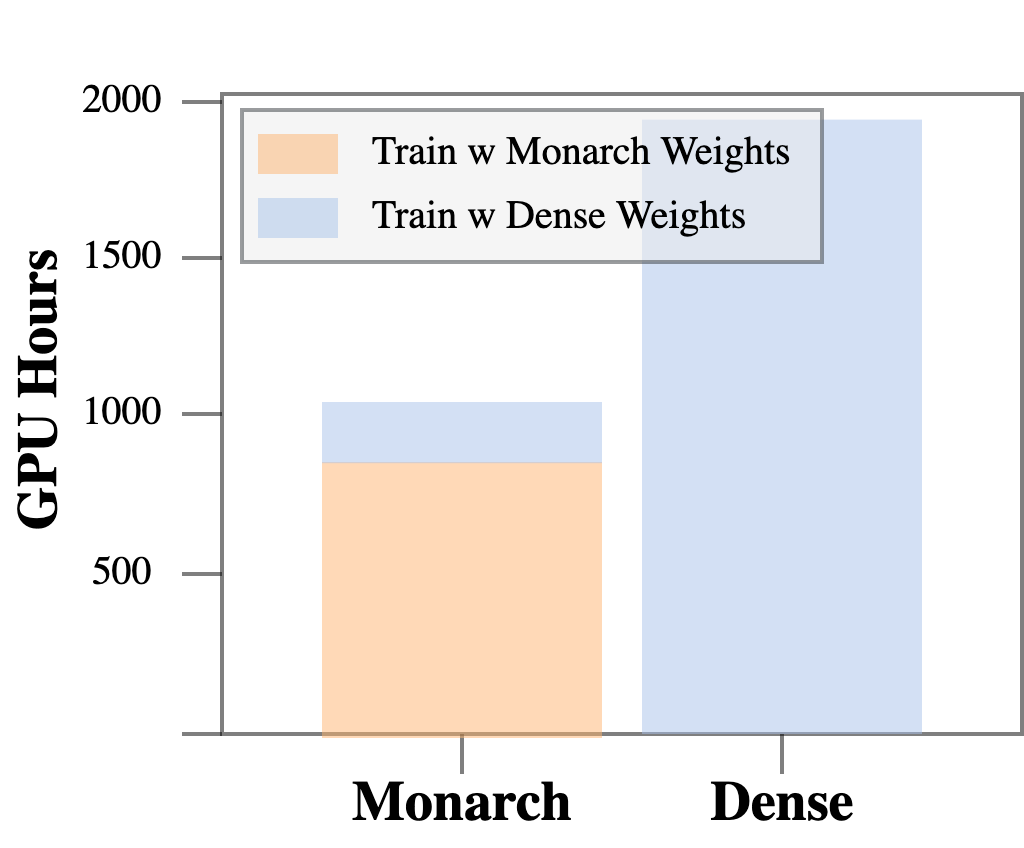
\includegraphics[width=.3\textwidth]{figures/rv_bar_temp.png}
  \vspace{-3mm}
  \caption{\label{fig:reverse_sparsification_bar}Time required (in A100 GPU hours) to reach the same perplexity (18.0)
    for GPT-2-small on OpenWebText.
    With ``reverse sparsification'', Monarch can speed up
    GPT-2 training by 2$\times$.\vspace{-1em}}
\end{figure}

We show that our Monarch approximation algorithm allows us to efficiently use
pretrained models, such as speeding up BERT finetuning on GLUE.

\paragraph{BERT finetuning.}
We take the BERT pretrained weights, approximate them with Monarch matrices,
and finetune the resulting model on the 9 GLUE tasks.
The results in \cref{table:bert_glue} shows that we obtain a Monarch finetuned
model with similar quality to the dense BERT model, but with 1.7$\times$ faster
finetuning speed.
This serves as a proof of concept, and we expect further speedup if additional model compression techniques are applied (e.g., quantization, kernel fusion).




\begin{table}[h]
  \small
  \centering
  \vspace{-5mm}
  \caption{\label{table:bert_glue}The performance of Monarch matrices in
    finetuning BERT on GLUE.}
  \setlength{\tabcolsep}{5pt}
  \vspace{1em}
  \iftoggle{arxiv}{}{
    \resizebox{\linewidth}{!}
  }
  {
  \begin{tabular}{@{}c||ccccccc@{}}
  \specialrule{.15em}{.05em}{.05em}
    Model&\multicolumn{1}{c}{GLUE (avg)}&\multicolumn{1}{c}{Speedup} &\multicolumn{1}{c}{Params} & \multicolumn{1}{c}{FLOPs} \\
    \specialrule{.15em}{.05em}{.05em}
    BERT-base & 78.6& - & 109M & 11.2G \\
    Monarch-BERT-base& 78.3& 1.5$\times$ & 55M & 6.2G  \\
    BERT-large & 80.4 & - & 335M & 39.5G \\
    Monarch-BERT-large & 79.6 & 1.7$\times$ & 144M & 14.6G  \\
    \specialrule{.15em}{.05em}{.05em}
  \end{tabular}
  }
  \vspace{-3mm}
\end{table}




\section*{Acknowledgements}
This work was supported by the ERC grant number 714381 (SOLARIS project) and by the MSR-Inria joint centre.

\bibliography{bibli}
\bibliographystyle{icml2019}

\newpage

\appendix
\onecolumn


Section~\ref{sec:experiments_appx} of this supplementary presents extended results
from our experiments, along with statistical tests for assessing the significance of our findings.
Section~\ref{sec:deformation_penalties} details our lower bound penalties based on deformations
and their relationship to tangent propagation.
Section~\ref{sec:spectral_norms_appx} presents our continuation algorithm for optimization
with spectral norm constraints.
Section~\ref{sec:non_euclidian_appx} describes
heuristic extensions of our lower bound regularization strategies to non-Euclidian geometries.
Finally, Section~\ref{sec:generalization_appx} provides our proof of the margin bound
of Proposition~\ref{prop:robust_margin_bound} for adversarial generalization.

\section{Additional Experiment Results}
\label{sec:experiments_appx}

\subsection{CIFAR10}
\label{sub:cifar_appx}

This section provides more extensive results for the experiments on CIFAR10 from Section~\ref{sub:exp_smalldata}.
In particular, Table~\ref{tab:smalldata_ext} shows additional experiments on larger subsets of size 5\.000,
as well as more methods, including different geometries (see Appendix~\ref{sec:non_euclidian_appx}).
The table also reports results obtained when using a smaller validation set of size 1\,000.
The full hyper-parameter grid is given in Table~\ref{tab:smalldata_param_grid}.

In order to assess the statistical significance of our results,
we repeated the experiments on 10 new random choices of subsets, using the hyperparameters selected
on the original subset from Table~\ref{tab:smalldata_ext} (except for learning rate, which is selected according to a different validation set for each subset).
We then compared pairs of methods using a paired t-test, with p-values shown in Table~\ref{tab:t_test}.
In particular, the results strengthen some of our findings, for instance, that $\|\nabla f \|^2$
should be preferred to the gradient penalty on the loss when there is no data augmentation,
and that combined upper+lower bound approaches tend to outperform the individual upper or lower
bound strategies.


\begin{table}[h]
\caption{Regularization on CIFAR10 with 1\,000 or 5\,000 examples for VGG-11 and ResNet-18.
Extended version of Table~\ref{tab:smalldata}.
Each entry shows the test accuracy with/without data augmentation when all hyper-parameters are optimized on a validation set of size 10\,000 (a) or 1\,000 (b),
and for the epoch with highest validation accuracy,
evaluating every 10 epochs (similar to early stopping).}
\centering
\vspace{0.2cm}
\label{tab:smalldata_ext}
(a) 10k examples in validation set

% python print_table.py --full
\begin{tabular}{ | l | c | c | c | c |  }
\hline
Method & 1k VGG-11 & 1k ResNet-18 & 5k VGG-11 & 5k ResNet-18 \\ \hline
\hline
No weight decay & 50.70 / 43.75 & 45.23 / 37.12 & 72.49 / 58.35 & 72.72 / 54.12 \\
Weight decay & 51.32 / 43.95 & 44.85 / 37.09 & 72.80 / 58.56 & 73.06 / 53.33 \\
SN penalty (PI) & 54.64 / 45.06 & 47.01 / 39.63 & 74.03 / 62.45 & 74.79 / 54.04 \\
SN penalty (SVD) & 53.44 / 46.06 & 47.26 / 37.94 & 74.53 / 62.93 & 75.59 / 54.98 \\
SN projection & 54.14 / \textbf{\color{darkgray}46.70} & 47.12 / 37.28 & 75.14 / 63.81 & 76.23 / 55.60 \\
VAT & 50.88 / 43.36 & 47.47 / 42.82 & 72.91 / 58.78 & 71.56 / 55.93 \\
PGD-$\ell_2$ & 51.25 / 44.40 & 45.80 / 41.87 & 73.18 / 58.98 & 72.53 / 55.92 \\
PGD-$\ell_\infty$ & 51.17 / 43.07 & 45.31 / 39.66 & 73.05 / 57.82 & 72.75 / 55.14 \\
grad-$\ell_2$ & \textbf{\color{darkgray}55.19} / 43.88 & \textbf{49.30} / \textbf{\color{darkgray}44.65} & \textbf{75.38} / 59.20 & 75.22 / 55.36 \\
grad-$\ell_1$ & 54.88 / 44.74 & \textbf{\color{darkgray}49.06} / 42.63 & \textbf{\color{darkgray}75.25} / 59.39 & 74.48 / 56.19 \\
\hline
$\|f\|_\delta^2$ penalty & 51.41 / 45.07 & 48.73 / 43.72 & 72.98 / 61.45 & 72.78 / 56.50 \\
$\|\nabla f\|^2$ penalty & 54.80 / 46.37 & \textbf{\color{darkgray}48.99} / \textbf{44.97} & 73.90 / 60.17 & 73.83 / \textbf{\color{darkgray}57.92} \\
PGD-$\ell_2$ + SN proj & 54.19 / \textbf{\color{darkgray}46.66} & 47.47 / 41.25 & 74.61 / \textbf{64.50} & \textbf{\color{darkgray}77.19} / 57.43 \\
grad-$\ell_2$ + SN proj & \textbf{55.32} / \textbf{46.88} & 48.73 / 42.78 & 75.11 / 63.54 & \textbf{77.73} / 57.09 \\
$\|f\|_\delta^2$ + SN proj & 54.02 / \textbf{\color{darkgray}46.72} & 48.12 / 43.56 & 74.55 / \textbf{\color{darkgray}64.33} & 75.64 / \textbf{59.03} \\
$\|\nabla f\|^2$ + SN proj & \textbf{55.24} / \textbf{46.80} & \textbf{\color{darkgray}49.06} / \textbf{44.92} & 72.31 / 63.74 & 72.24 / 57.56 \\
\hline
\end{tabular}
\\
\vspace{0.2cm}
(b) 1k examples in validation set

% python print_table.py --full --small_val
\begin{tabular}{ | l | c | c | c | c |  }
\hline
Method & 1k VGG-11 & 1k ResNet-18 & 5k VGG-11 & 5k ResNet-18 \\ \hline
\hline
No weight decay & 51.32 / 43.42 & 45.00 / 37.00 & 72.64 / 57.88 & 72.71 / 53.80 \\
Weight decay & 51.04 / 43.42 & 44.66 / 36.77 & 72.68 / 57.59 & 72.25 / 54.16 \\
SN penalty (PI) & 54.60 / 44.20 & 46.39 / 38.86 & 72.99 / 62.49 & 74.72 / 53.65 \\
SN penalty (SVD) & 53.76 / 44.79 & 47.31 / 37.92 & 74.05 / 63.34 & 75.73 / 54.65 \\
SN projection & 52.86 / \textbf{\color{darkgray}46.49} & 47.05 / 37.28 & 74.18 / \textbf{\color{darkgray}63.70} & 75.91 / 54.43 \\
VAT & 50.90 / 43.99 & 47.35 / 42.91 & 72.95 / 57.64 & 71.91 / 55.22 \\
PGD-$\ell_2$ & 50.95 / 43.26 & 45.77 / 41.71 & 72.71 / 57.68 & 72.87 / 54.17 \\
PGD-$\ell_\infty$ & 51.16 / 43.16 & 45.67 / 39.77 & 73.64 / 58.02 & 72.99 / 53.95 \\
grad-$\ell_2$ & \textbf{55.40} / 43.57 & 47.86 / \textbf{\color{darkgray}44.65} & \textbf{75.44} / 58.33 & 74.83 / 55.43 \\
grad-$\ell_1$ & 54.53 / 43.04 & \textbf{\color{darkgray}48.75} / 42.21 & \textbf{\color{darkgray}75.28} / 58.19 & 74.28 / 54.02 \\
\hline
$\|f\|_M^2$ penalty & 51.00 / 44.67 & 48.57 / 44.30 & 72.76 / 60.55 & 72.75 / 56.49 \\
$\|\nabla f\|^2$ penalty & 54.68 / 46.10 & 48.53 / \textbf{45.21} & 73.83 / 60.36 & 73.30 / \textbf{\color{darkgray}57.46} \\
PGD-$\ell_2$ + SN proj & 53.85 / \textbf{46.79} & 46.48 / 40.95 & 74.79 / 63.37 & \textbf{\color{darkgray}76.28} / \textbf{\color{darkgray}57.43} \\
grad-$\ell_2$ + SN proj & \textbf{\color{darkgray}55.28} / 45.11 & 48.42 / 41.93 & 75.17 / 63.45 & \textbf{77.24} / 56.18 \\
$\|f\|_M^2$ + SN proj & 54.00 / 45.14 & 47.12 / 41.86 & 74.54 / \textbf{63.94} & 75.25 / \textbf{57.94} \\
$\|\nabla f\|^2$ + SN proj & \textbf{\color{darkgray}55.21} / 45.68 & \textbf{49.03} / 43.58 & 71.92 / 63.47 & 71.83 / 56.06 \\
\hline
\end{tabular}
\end{table}


\begin{table}[h]
\caption{Paired t-tests comparing pairs of methods, on 10 different random choices of subsets of CIFAR10.
Each cell shows the p-value of the corresponding test, both with (left) and without (right) data augmentation.
We only show p-values smaller than~$0.05$.
Hyperparameters are fixed to the ones obtained for the results in Table~\ref{tab:smalldata}
(selected on a different choice of subset), except for the learning rate which is tuned on
a separate validation set for each choice of subset.}
\centering
\label{tab:t_test}
\vspace{0.2cm}
% python print_significance_table.py --test_type ttest --optlr
\begin{tabular}{ | c | c c | c c | c c | c c |  }
\hline
Test & \multicolumn{2}{|c|}{1k VGG-11} & \multicolumn{2}{|c|}{1k ResNet-18} & \multicolumn{2}{|c|}{5k VGG-11} & \multicolumn{2}{|c|}{5k ResNet-18} \\ \hline
\hline
SN projection $\succ$ Weight decay & 1e-04 & 1e-03 & - & - & 3e-06 & 1e-08 & 9e-07 & 4e-04\\ \hline
grad-$\ell_2$ $\succ$ Weight decay & 4e-09 & - & 2e-04 & 5e-05 & 7e-08 & 1e-04 & 5e-06 & -\\ \hline
$\|\nabla f\|^2$ $\succ$ Weight decay & 1e-08 & 2e-07 & 1e-05 & 3e-07 & 3e-04 & 5e-07 & 7e-03 & 1e-06\\ \hline
$\|\nabla f\|^2$ $\succ$ grad-$\ell_2$ & - & 3e-08 & 2e-02 & 2e-06 & - & 6e-05 & - & 4e-05\\ \hline
grad-$\ell_2$ $\succ$ $\|\nabla f\|^2$ & 2e-02 & - & - & - & 2e-05 & - & 7e-04 & -\\ \hline
grad-$\ell_2$ + SN proj $\succ$ grad-$\ell_2$ & - & 9e-03 & - & - & - & 5e-07 & 9e-06 & 2e-04\\ \hline
$\|\nabla f\|^2$ + SN proj $\succ$ $\|\nabla f\|^2$ & - & - & - & 1e-02 & - & 2e-06 & - & -\\ \hline
\end{tabular}
\end{table}

\begin{table}[h]
\caption{List of hyper-parameters used for each method on CIFAR10.
For each method, we additionally consider a learning rate parameter in $[0.003 ; 0.01 ; 0.03 ; 0.1]$.
For combined penalties, the sets of hyperparameters are listed in the same order as in the first column
(\ie, the choices of constraint radius are given last).}
\centering
\small
\vspace{0.2cm}
\label{tab:smalldata_param_grid}
\begin{tabular}{ | l | c |  }
\hline
Method & Parameter grid \\ \hline
\hline
No weight decay &  -   \\ \hline
Weight decay &  $[0; 0.0001 ; 0.0002 ; 0.0004 ; 0.0008 ; 0.001 ; 0.002]$   \\ \hline
SN penalty (PI) &  $[0.001 ; 0.003 ; 0.01 ; 0.03 ; 0.1 ; 0.3]$ \\ \hline
SN penalty (SVD) &  $[0.001 ; 0.003 ; 0.01 ; 0.03 ; 0.1 ; 0.3]$  \\ \hline
SN projection &  $[0.5 ; 0.6 ; 0.8 ; 1.0 ; 1.2 ; 1.4]$  \\ \hline
$\|f\|_\delta^2$ penalty & $[0.001 ; 0.003 ; 0.01 ; 0.03 ; 0.1]$  \\ \hline
$\|\nabla f\|^2$ penalty & $[0.00003 ; 0.0001 ; 0.0003 ; 0.001 ; 0.003 ; 0.01 ; 0.03]$ \\ \hline
VAT & $[0.1 ; 0.3 ; 1.0 ; 3.0]$ \\ \hline
PGD-$\ell_2$ &  $[0.003 ; 0.01 ; 0.03 ; 0.1 ; 0.3 ; 1.0]$ \\ \hline
PGD-$\ell_\infty$ &  $[0.001 ; 0.003 ; 0.01 ; 0.03 ; 0.1 ; 0.3]$  \\ \hline
grad-$\ell_1$ &  $[0.0001 ; 0.0003 ; 0.001 ; 0.003 ; 0.01 ; 0.03]$  \\ \hline
grad-$\ell_2$ &  $[0.001 ; 0.003 ; 0.01 ; 0.03 ; 0.1 ; 0.3 ; 1.0 ; 3.0]$ \\ \hline
PGD-$\ell_2$ + SN projection &  $ [0.003 ; 0.01 ; 0.03 ; 0.1] \times [0.6 ; 1.0 ; 1.4]$   \\ \hline
grad-$\ell_2$ + SN projection & $ [0.003 ; 0.01 ; 0.03 ; 0.1] \times [0.6 ; 1.0 ; 1.4]$  \\ \hline
$\|f\|_\delta^2$ + SN projection & $ [0.003 ; 0.01 ; 0.03] \times [0.6 ; 1.0 ; 1.4]$    \\ \hline
$\|\nabla f\|^2$ + SN projection & $ [0.001 ; 0.01 ; 0.1] \times [0.6 ; 1.0 ; 1.4]$   \\ \hline
\end{tabular}
\end{table}

\subsection{Infinite MNIST}
\label{sub:imnist_appx}

We provide more extensive results for the Infinite MNIST dataset in Table~\ref{tab:imnist_ext},
in particular showing more regularization strategies, as well as results with or without
data augmentation, marked with~$(\ast)$.
As in the case of CIFAR10, we use SGD with momentum (fixed to 0.9) for 500 epochs,
with initial learning rates in~$[0.005; 0.05; 0.5]$, and divide the step-size by 2 every 40 epochs.
The full hyper-parameter grid is given in Table~\ref{tab:imnist_param_grid}.


As in the case of CIFAR10, we report statistical significance tests in Table~\ref{tab:imnist_ttests} comparing pairs of
methods based on 10 different random choices of subsets.
In particular, the results confirm that weight decay with data augmentation alone
tends to give weaker results than separate penalties,
and that the combined penalty $\|f\|_\tau^2 + \|f\|_\delta^2$, which combines adversarial
perturbations of two different types,
outperforms each penalty taken by itself on a single type of perturbation,
which emphasizes the benefit of considering perturbations of different natures,
perhaps thanks to a tighter lower bound approximation of the RKHS norm.
We note that grad-$\ell_2 (\ast)$ worked well on some subsets,
but poorly on others due to training instabilities,
possibly because of the selected hyperparameters which are quite large
(and thus likely violate the approximation to the robust optimization objective).

\begin{table}
\caption{Test accuracies on subsets of MNIST using deformations from Infinite MNIST.
Extended version of Table~\ref{tab:imnist}.
($\ast$) indicates that random deformations were included as training examples (\ie, data augmentation),
while $\|f\|_\tau^2$ and $\|D_\tau f\|^2$
use them as part of the regularization penalty.
As in Table~\ref{tab:smalldata_ext}, we show results obtained using a validation set
of size 10\,000 (a) and 1\,000 (b).
}
\centering
\vspace{0.2cm}
\label{tab:imnist_ext}
\begin{tabular}{c c}
(a) 10k examples in validation set
& (b) 1k examples in validation set \\

% python print_table_imnist.py --lr --appendix
\begin{tabular}{ | l | c | c |  }
\hline
Method & 300 VGG & 1k VGG \\ \hline
\hline
Weight decay & 89.32 & 94.08 \\
Weight decay ($\ast$) & 92.41 & 95.64 \\
SN projection & 90.69 & 95.01 \\
SN projection ($\ast$) & 92.17 & 95.88 \\
grad-$\ell_2$ & 93.63 & 96.67 \\
grad-$\ell_2$ ($\ast$) & 95.05 & 97.48 \\
\hline
$\|f\|_\delta^2$ penalty & 94.17 & 96.99 \\
$\|f\|_\delta^2$ penalty ($\ast$) & 94.86 & 97.40 \\
$\|\nabla f\|^2$ penalty & 94.08 & 96.82 \\
$\|\nabla f\|^2$ penalty ($\ast$) & 94.80 & 97.29 \\
$\|D_\tau f\|^2$ penalty & 94.18 & 96.98 \\
$\|D_\tau f\|^2$ penalty ($\ast$) & 94.91 & 97.29 \\
$\|f\|_\tau^2$ penalty & 94.42 & 97.13 \\
$\|f\|_\tau^2$ penalty ($\ast$) & 94.83 & 97.25 \\
$\|f\|_{\tau}^2$ + $\|\nabla f\|^2$ & 94.75 & 97.40 \\
$\|f\|_{\tau}^2$ + $\|\nabla f\|^2$ ($\ast$) & 95.14 & 97.44 \\
$\|f\|_{\tau}^2$ + $\|f\|^2_\delta$ & 95.23 & \textbf{\color{darkgray}97.66} \\
$\|f\|_{\tau}^2$ + $\|f\|^2_\delta$ ($\ast$) & \textbf{95.53} & \textbf{\color{darkgray}97.56} \\
grad-$\ell_2$ + SN proj & 93.89 & 96.85 \\
grad-$\ell_2$ + SN proj ($\ast$) & 95.15 & \textbf{97.80} \\
$\|f\|_\delta^2$ + SN proj & 93.97 & 96.89 \\
$\|f\|_\delta^2$ + SN proj ($\ast$) & 94.78 & 97.38 \\
$\|f\|_{\tau}^2$ + $\|\nabla f\|^2$ + SN proj & 95.09 & 97.42 \\
$\|f\|_{\tau}^2$ + $\|\nabla f\|^2$ + SN proj ($\ast$) & 95.03 & 97.27 \\
$\|f\|_{\tau}^2$ + $\|f\|^2_\delta$ + SN proj & 95.20 & \textbf{\color{darkgray}97.60} \\
$\|f\|_{\tau}^2$ + $\|f\|^2_\delta$ + SN proj ($\ast$) & \textbf{\color{darkgray}95.40} & \textbf{97.77} \\
\hline
\end{tabular}
&
% python print_table_imnist.py --lr --appendix --small_val
\begin{tabular}{ | l | c | c |  }
\hline
Method & 300 VGG & 1k VGG \\ \hline
\hline
Weight decay & 89.32 & 93.34 \\
Weight decay ($\ast$) & 91.91 & 95.73 \\
SN projection & 90.60 & 94.83 \\
SN projection ($\ast$) & 92.01 & 95.91 \\
grad-$\ell_2$ & 92.92 & 96.42 \\
grad-$\ell_2$ ($\ast$) & \textbf{\color{darkgray}94.69} & \textbf{\color{darkgray}97.48} \\
\hline
$\|f\|_M^2$ penalty & 93.44 & 96.98 \\
$\|f\|_M^2$ penalty ($\ast$) & 94.57 & 97.14 \\
$\|\nabla f\|^2$ penalty & 94.08 & 96.77 \\
$\|\nabla f\|^2$ penalty ($\ast$) & 94.50 & 97.15 \\
$\|D_\tau f\|^2$ penalty & 94.03 & 97.16 \\
$\|D_\tau f\|^2$ penalty ($\ast$) & 94.15 & 96.64 \\
$\|f\|_\tau^2$ penalty & 93.53 & 97.13 \\
$\|f\|_\tau^2$ penalty ($\ast$) & \textbf{\color{darkgray}94.79} & 97.26 \\
$\|f\|_{\tau}^2$ + $\|\nabla f\|^2$ & \textbf{\color{darkgray}94.75} & 97.21 \\
$\|f\|_{\tau}^2$ + $\|\nabla f\|^2$ ($\ast$) & 94.43 & \textbf{\color{darkgray}97.42} \\
$\|f\|_{\tau}^2$ + $\|f\|^2_M$ & \textbf{95.15} & 97.27 \\
$\|f\|_{\tau}^2$ + $\|f\|^2_M$ ($\ast$) & \textbf{95.20} & \textbf{\color{darkgray}97.49} \\
grad-$\ell_2$ + SN proj & 93.44 & 96.81 \\
grad-$\ell_2$ + SN proj ($\ast$) & 94.05 & \textbf{97.60} \\
$\|f\|_M^2$ + SN proj & 93.97 & 96.61 \\
$\|f\|_M^2$ + SN proj ($\ast$) & \textbf{\color{darkgray}94.69} & 97.33 \\
$\|f\|_{\tau}^2$ + $\|\nabla f\|^2$ + SN proj & \textbf{\color{darkgray}94.75} & 97.16 \\
$\|f\|_{\tau}^2$ + $\|\nabla f\|^2$ + SN proj ($\ast$) & \textbf{\color{darkgray}94.74} & 97.22 \\
$\|f\|_{\tau}^2$ + $\|f\|^2_M$ + SN proj & \textbf{\color{darkgray}94.78} & \textbf{\color{darkgray}97.49} \\
$\|f\|_{\tau}^2$ + $\|f\|^2_M$ + SN proj ($\ast$) & \textbf{95.17} & \textbf{97.64} \\
\hline
\end{tabular}
\end{tabular}
\end{table}

\begin{table}
\caption{Paired t-tests comparing pairs of methods,
on 10 different random choices of subsets of MNIST.
Each cell shows the p-value of the corresponding test.
We only show p-values smaller than~$0.05$.
Hyperparameters are fixed to the ones obtained for the results in Table~\ref{tab:imnist}
(selected on a different choice of subset), except for the learning rate which is tuned on
a separate validation set for each choice of subset.
}
\centering
\vspace{0.2cm}
\label{tab:imnist_ttests}
% python print_significance_table_imnist.py --test_type ttest --optlr
\begin{tabular}{ | c | c | c |  }
\hline
Test & 300 VGG & 1k VGG \\ \hline
\hline
grad-$\ell_2$ ($\ast$) $\succ$ Weight decay ($\ast$) & - & 3e-11\\ \hline
$\|f\|_\tau^2$ penalty $\succ$ Weight decay ($\ast$) & 2e-08 & 2e-10\\ \hline
$\|f\|_{\tau}^2$ + $\|f\|^2_\delta$ $\succ$ Weight decay ($\ast$) & 1e-08 & 2e-10\\ \hline
$\|f\|_{\tau}^2$ + $\|f\|^2_\delta$ + SN proj ($\ast$) $\succ$ grad-$\ell_2$ ($\ast$) & - & 1e-02\\ \hline
grad-$\ell_2$ ($\ast$) $\succ$ $\|f\|_{\tau}^2$ + $\|f\|^2_\delta$ + SN proj ($\ast$) & - & -\\ \hline
$\|f\|_{\tau}^2$ + $\|f\|^2_\delta$ $\succ$ $\|f\|_\delta^2$ penalty & 1e-07 & 6e-09\\ \hline
$\|f\|_{\tau}^2$ + $\|f\|^2_\delta$ $\succ$ $\|f\|_\tau^2$ penalty & 2e-06 & 6e-07\\ \hline
$\|f\|_{\tau}^2$ + $\|f\|^2_\delta$ ($\ast$) $\succ$ $\|f\|_{\tau}^2$ + $\|f\|^2_\delta$ & 2e-03 & -\\ \hline
$\|f\|_{\tau}^2$ + $\|f\|^2_\delta$ + SN proj ($\ast$) $\succ$ $\|f\|_{\tau}^2$ + $\|f\|^2_\delta$ & 2e-03 & 2e-04\\ \hline
\end{tabular}
\end{table}


\begin{table}
\caption{List of hyper-parameters used for each method on Infinite MNIST.
For each method, we additionally consider a learning rate parameter in $[0.005 ; 0.05 ; 0.5]$.
For combined penalties, the sets of hyperparameters are listed in the same order as in the first column
(\eg, the choices of constraint radius are given last).}
\centering
\small
\vspace{0.2cm}
\label{tab:imnist_param_grid}
\begin{tabular}{ | l | c | }
\hline
Method & Grid \\ \hline
\hline
Weight decay & [0; 0.00001; 0.00003; 0.0001; 0.0003; 0.001; 0.003; 0.01; 0.03; 0.1] \\
SN projection & [1.0; 1.2; 1.4; 1.6; 1.8] \\
grad-$\ell_2$ & [0.1; 0.3; 1.0; 3.0; 10.0] \\
$\|f\|_\delta^2$ penalty & [0.1; 0.3; 1.0; 3.0] \\
$\|\nabla f\|^2$ penalty & [0.0003; 0.001; 0.003; 0.01; 0.03; 0.1; 0.3] \\
$\|D_\tau f\|^2$ penalty & [0.003; 0.01; 0.03; 0.1; 0.3] \\
$\|f\|_\tau^2$ penalty & [0.03; 0.1; 0.3; 1.0; 3.0] \\
$\|f\|_{\tau}^2$ + $\|\nabla f\|^2$ & [0.03; 0.1; 0.3; 1.0] $\times$ [0.003; 0.01; 0.03; 0.1] \\
$\|f\|_{\tau}^2$ + $\|f\|^2_\delta$ & [0.1; 0.3; 1.0] $\times$ [0.03; 0.1] \\
grad-$\ell_2$ + SN proj & [0.3; 1.0; 3.0; 10.0; 30.0] $\times$ [1.2; 1.6; 2.0] \\
$\|f\|_\delta^2$ + SN proj & [0.03; 0.1] $\times$ [1.2; 1.6; 2.0] \\
$\|f\|_{\tau}^2$ + $\|\nabla f\|^2$ + SN proj & [0.03; 0.1; 0.3] $\times$ [0.01; 0.03; 0.1] $\times$ [1.2; 1.6; 2.0] \\
$\|f\|_{\tau}^2$ + $\|f\|^2_\delta$ + SN proj & [0.1; 0.3; 1.0] $\times$ [0.03; 0.1] $\times$ [1.2; 1.6; 2.0] \\
\hline
\end{tabular}
\end{table}

\subsection{Protein homology detection}
\label{sub:protein_appx}

\paragraph{Dataset description.}
Our protein homology detection experiments consider
the Structural Classification Of Proteins (SCOP) version 1.67 dataset \citep{murzin1995scop},
filtered and split following the procedures of \cite{haandstad2007motif}.
Specifically, positive training samples are extracted from one superfamily from which one family is withheld to serve as positive test set, while negative sequences are chosen from outside of the target family’s hold and are randomly split into training and test samples in the same ratio as positive samples.
This yields 102 superfamily classification tasks, which are generally very class-imbalanced.
For each task, we sample 100 class-balanced training samples to use as training set. The positive samples are extended to 50 with Uniref50 using PSI-BLAST \citep{altschul1997gapped} if they are fewer.

\paragraph{Data augmentation procedure.}
We consider in our experiments a discrete way of perturbing training samples to 
perform data augmentation. Specifically, for a given sequence, a perturbed sequence 
can be obtained by randomly changing some of the characters. Each character in the sequence 
is switched to a different one, randomly chosen from the alphabet, with some 
probability $p$. We fixed this probability to 0.1 throughout the experiments.

\paragraph{Experimental details and significance tests.}
In our experiments, we use the Adam optimization algorithm with a learning rate fixed
to 0.01 (and $\beta$ fixed to defaults $(0.9, 0.999)$),
with a batch size of 100 for 300 epochs.
The full hyper-parameter grid is given in Table~\ref{tab:protein_param_grid}.
In addition to the average auROC50 scores reported in Table~\ref{tab:protein},
we perform paired t-tests for comparing pairs of methods in Table~\ref{tab:protein_ttests}
in order to verify the significance of our findings.
The results confirm that the adversarial perturbation penalty and its combination
with spectral norm constraints tends to outperform the other approaches.


\begin{table}
\caption{Paired t-tests comparing pairs of methods on the 51 test datasets from the
set of protein homology detection tasks.
Each cell shows the p-value of the corresponding test.
We only show p-values smaller than~$0.05$.
We use the same hyperparameters as the ones obtained in the results of Table~\ref{tab:protein}.
}
\centering
\vspace{0.2cm}
\label{tab:protein_ttests}
\begin{tabular}{|l|c|c|}
\hline
 Test                                                            &   No DA &      DA \\ \hline
\hline
 SN proj $\succ$ Weight decay                                    &   1e-05 &   4e-05 \\
 grad-$\ell_2$ $\succ$ Weight decay                              &   5e-05 &   5e-02 \\
 $\|f\|_{\delta}^2$ $\succ$ Weight decay                         &   5e-06 &   3e-05 \\
 $\|\nabla f\|^2$ $\succ$ Weight decay                           &   9e-06 &   3e-03 \\
 $\|f\|_{\delta}^2$ $\succ$ grad-$\ell_2$                        &   -     &   4e-03 \\
 $\|\nabla f\|^2$ $\succ$ grad-$\ell_2$                          &   -     &   -     \\
 grad-$\ell_2$ + SN proj $\succ$ grad-$\ell_2$                   &   -     &   1e-03 \\
 $\|f\|_{\delta}^2$ + SN proj $\succ$ $\|f\|_{\delta}^2$         &   3e-03 &   5e-02 \\
 $\|\nabla f\|^2$ + SN proj $\succ$ $\|\nabla f\|^2$             &   -     &   -     \\
 $\|f\|_{\delta}^2$ + SN proj $\succ$ $\|\nabla f\|^2$ + SN proj &   8e-05 &   -     \\
\hline
\end{tabular}
\end{table}

\begin{table}
\caption{List of hyper-parameters used for each method on protein homology detection datasets.
For combined penalties, the hyperparameters are the cross-products of each individual method.}
\centering
\small
\vspace{0.2cm}
\label{tab:protein_param_grid}
\begin{tabular}{|c|c|}
\hline
 Method                                                       &   Parameter grid \\ \hline
\hline
 No weight decay  &  $-$                          \\
 Weight decay     &  $[0; 0.01; 0.001; 0.0001; 0.00001]$ \\
 SN proj          &  $[10; 1.0; 0.1]$             \\
 PGD-$\ell_2$     &  $[100.0; 10.0; 1.0; 0.1]$    \\
 grad-$\ell_2$    &  $[100.0; 10.0; 1.0; 0.1; 0.01, 0.001]$     \\
 $\|f\|_{\delta}^2$      &  $[10.0; 1.0; 0.1]$           \\
 $\|\nabla f\|^2$ &  $[10.0; 1.0; 0.1; 0.01; 0.001; 0.0001]$ \\
\hline
\end{tabular}
\end{table}


\subsection{Robustness}
\label{sub:robustness_appx}

Figure~\ref{fig:robust_tradeoffs_appx} extends Figure~\ref{fig:robust_tradeoffs}
from Section~\ref{sub:exp_robust} to show more methods, adversary strenghts, and different geometries.
For combined (PGD-$\ell_2$ + SN projection) approaches, we can see that stronger constraints (\ie, smaller~$\tau$)
tend to reduce standard accuracy, likely because it prevents a good fit of the data,
but can provide better robustness to strong adversaries ($\epsilon_{test} = 1$).
We can see that using the right metric in PGD indeed helps against an~$\ell_\infty$ adversary,
nevertheless controlling global stability through the RKHS norm as in the~$\|f\|_\delta^2$ and~$\|\nabla f\|^2$
penalties can still provide some robustness against such adversaries, even with large $\epsilon_{test}$.
For gradient penalties, we find that the different geometries behave quite similarly,
which may suggest that more appropriate optimization algorithms than SGD could be needed to
better accommodate the non-smooth case of $\ell_1/\ell_\infty$, or perhaps that both algorithms are actually
controlling the same notion of complexity on this dataset.


\begin{figure*}
	\centering
	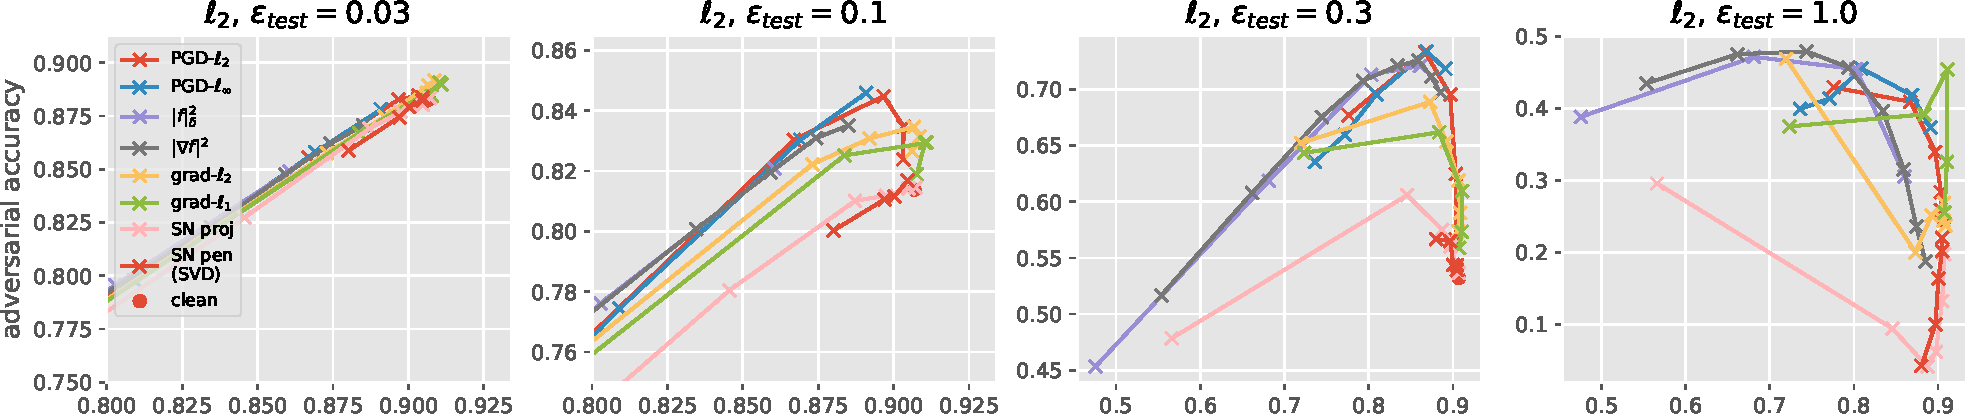
\includegraphics[width=.9\textwidth]{figures/cifar10_vgg/test_vs_adv_l2.pdf}
	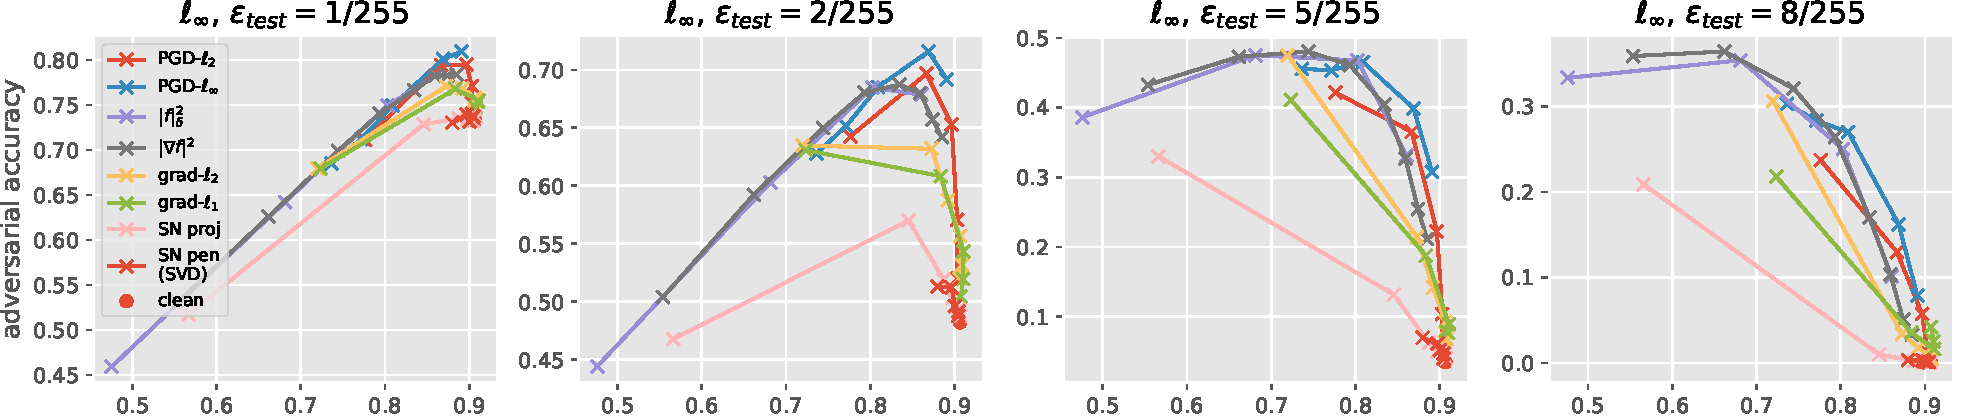
\includegraphics[width=.9\textwidth]{figures/cifar10_vgg/test_vs_adv_linf.pdf}
	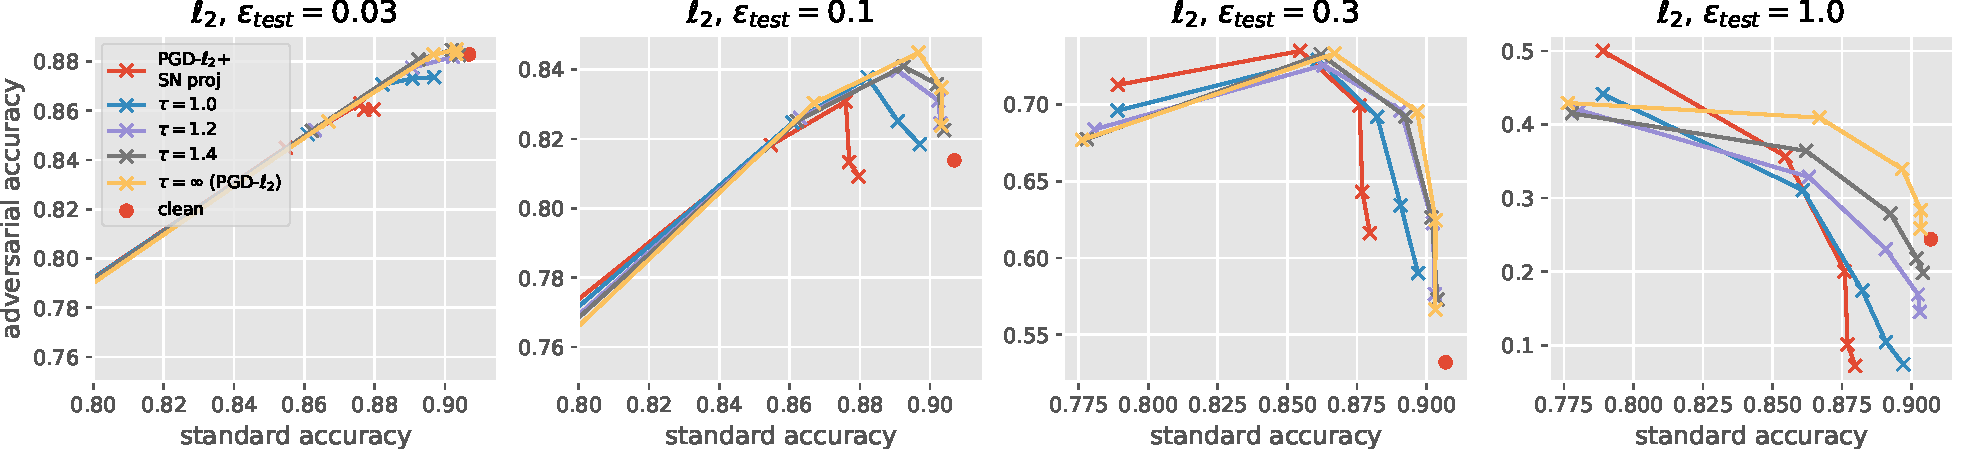
\includegraphics[width=.9\textwidth]{figures/cifar10_vgg/test_vs_adv_comb.pdf}
	\caption{Robustness trade-off curves of different regularization methods for VGG11 on CIFAR10 (extended
	version of Figure~\ref{fig:robust_tradeoffs}).
	The plots show test accuracy vs adversarial test accuracy
	for $\ell_2$-bounded (top/bottom) or $\ell_\infty$-bounded (middle),
	40-step PGD adversaries with a fixed~$\epsilon_{\text{test}}$.
	Different points on a curve correspond to training with different regularization strengths.
	The regularization increases monotonically along a given curve, and
	the leftmost points correspond to the strongest regularization.
	The bottom plots consider PGD-$\ell_2$ + SN projection,
	with different fixed values of the constraint radius~$\tau$, for varying $\epsilon$ in PGD.}
	\label{fig:robust_tradeoffs_appx}
\end{figure*}


\clearpage

\section{Details on Deformation Stability Penalties}
\label{sec:deformation_penalties}
%!TEX root = main.tex

This section provides more details on the deformation stability penalties mentioned in
Section~\ref{sub:lower_bounds}, and the practical versions we use in our experiments on the
Infinite MNIST dataset~\citep{loosli-canu-bottou-2006}.

\paragraph{Stability to deformations.}
We begin by providing some background on deformation stability,
recalling that these can provide new lower bound penalties as explained in Section~\ref{sub:lower_bounds}.
Viewing an element $x \in \mathcal X$ as a signal $x(u)$, where $u$ denotes the location
(\eg~a two-dimensional vector for images),
we denote by $x_\tau$ a deformed version of~$x$ given by $x_\tau(u) = x(u - \tau(u))$,
where~$\tau$ is a diffeomorphism.
The deformation stability bounds of~\citet{bietti2018group} take the form:
\begin{equation}
\label{eq:stability_bound}
\|\Phi(x_\tau) - \Phi(x)\|_\Hcal \leq (C_1 \|\tau\|_\infty + C_2 \|\nabla \tau\|_\infty) \|x\|,
\end{equation}
where $\nabla \tau (u)$ is the Jacobian of $\tau$ at location~$u$.
Here, $C_1$ controls translation invariance and typically decreases with the total amount of pooling
(\ie, translation invariance more or less corresponds to the resolution at the final layer),
while~$C_2$ controls stability to deformations (note that $\nabla \tau = 0$ for translations)
and is typically smaller when using small patches.
We note that the bounds assume linear pooling layers with a certain spatial decay,
adapted to the resolution of the current layer;
our experiments on Infinite MNIST with deformation stability penalties
thus use average pooling layers on 2x2 neighborhoods.


\paragraph{Adversarial deformation penalty.}
We can obtain lower bound penalties by exploiting the above stability bounds in
a similar manner to the adversarial perturbation penalty introduced in Section~\ref{sub:lower_bounds}.
In particular, assuming a scalar-valued convolutional network~$f$:
\begin{equation}
\label{eq:adv_deformation}
\|f\|_\tau^2 := \sup_{x \in \mathcal X, \tau \in \mathcal T} (f(x_\tau) - f(x))^2 \\
\end{equation}
where~$\mathcal T$ is a collection of diffeomorphisms.
When the diffeomorphisms in~$\mathcal T$ have bounded norm~$\|\tau\|_\infty$ and
Jacobian norm~$\|\nabla \tau\|_\infty$,
and assuming $\mathcal X$ (or, in practice, the training data) is bounded,
the stability bound~\ref{eq:stability_bound} ensures that
the set $U_{\mathcal T} = \{\Phi(x_\tau) - \Phi(x) : x \in \mathcal X, \tau \in \mathcal T\}$ is included in an
RKHS ball with some radius $r$, so that~$\|f\|_\tau$ is a lower bound on~$r \|f\|_\Hcal$.

\paragraph{Tangent gradient penalty.}
We also consider the following gradient penalty along tangent vectors,
which provides an approximation of the above adversarial penalty when
considering small, parameterized deformations,
and recovers the tangent propagation strategy of~\citet{simard1998transformation}:
\begin{equation}
\label{eq:tangent_gradient}
\|D_\tau f\|^2 := \sup_{x \in \mathcal X} \|\partial_\alpha f(x + \sum_i \alpha_i t_{x,i}) \|^2,
\end{equation}
where $\{t_{x,i}\}_{i=1,\ldots, q}$ are
tangent vectors at~$x$ obtained from a given set of deformations.
To see the link with the adversarial deformation penalty~\ref{eq:adv_deformation},
consider for simplicity a single deformation,~$\mathcal T = \{\tau_0\}$.
For small~$\alpha$, we have
\begin{align*}
x_{\alpha \tau_0} \approx x + \alpha t_x, \quad \text{where} \quad t_x(u) = \tau_0(u) \cdot \nabla x(u),
\end{align*}
where~$t_x$ denotes the tangent vector of the deformation
manifold $\{\alpha \tau_0 : \alpha\}$ at~$\alpha = 0$~\citep{simard1998transformation}.
Then,
\[
f(x_{\alpha\tau_0}) - f(x) \approx \alpha \partial_\alpha f(x + \alpha t_x) = \alpha \langle \nabla f(x), t_x \rangle.
\]
In this case, denoting $\alpha \mathcal T = \{\alpha \tau_0\}$, we have
\[
\sup_{x \in \mathcal X, \tau \in \alpha \mathcal T} (f(x_\tau) - f(x))^2 \approx \alpha^2 \sup_{x \in \mathcal X} |\partial_\alpha f(x + \alpha t_x)|^2,
\]
so that when $\alpha$ is small, the adversarial penalty can be approximated by $\alpha \|D_\tau f\|$
(note that using $\alpha \mathcal T$ instead of~$\mathcal T$ in the adversarial penalty
would also yield a scaling by~$\alpha$, since the stability bounds imply $\alpha$ times smaller
perturbations in the RKHS).

\paragraph{Practical implementations on Infinite MNIST.}
In our experiments on Infinite MNIST, we compute $\|f\|_\tau^2$ by considering 32 random transformations
of each digit in a mini-batch of training examples,
and taking the maximum over both the example and the transformation.
We do this separately for each class, as for the other lower bound penalties $\|f\|_\delta^2$ and $\|\nabla f\|^2$.
For~$\|D_\tau f\|^2$, we take $\{t_{x,i}\}_{i=1,\ldots,q}$ with~$q=30$ to be tangent vectors given
by random diffeomorphisms from Infinite MNIST around each example~$x$.


\section{Details on Optimization with Spectral Norms}
\label{sec:spectral_norms_appx}
%!TEX root = main.tex
%\subsection{Derivation of the proximal operator for solving %\eqref{eq:optimization_problem_penalized}}
%\label{sub:proximal_method}
%The proximal operator of \eqref{eq:optimization_problem_penalized} is, for $x \in \mathrm{R}^d$ :
%\begin{equation*}
%\label{prox_operator}
%\text{prox}_{\gamma\|.\|_{\infty}}(x) = x - \text{proj}_{\|.\|_1 \leq \gamma}(x),
%\end{equation*}
%with $\gamma>0$.
%\begin{proof}
%Using the generalized Moreau's decomposition and knowing that Fenchel's conjugate of the infinity norm %is the indicator function of the $l_1$-ball, we get :
%\begin{align*}
%x &= \text{prox}_{\gamma\|.\|_{\infty}}(x) + %\gamma\text{prox}_{\frac{\|.\|_{\infty}^*}{\gamma}}(\frac{x}{\gamma}) \\
%&= \text{prox}_{\gamma\|.\|_{\infty}}(x) + %\gamma\text{prox}_{\frac{{\mathbf{1}}_{\|.\|_{1}}}{\gamma}}(\frac{x}{\gamma}).
%\end{align*}
%As a consequence,
%\begin{align*}
%\text{prox}_{\gamma\|.\|_{\infty}}(x) &= x - %\gamma\text{prox}_{\frac{{\mathbf{1}}_{\|.\|_{1}}}{\gamma}}(\frac{x}{\gamma}) \\
%&= x - \gamma\text{argmin}_{u \in \mathrm{R}^d}\left(\frac{1}{2}\|u-\frac{x}{\gamma}\|_{2}^2 + %\frac{{\mathbf{1}}_{\|u\|_{1} \leq 1}}{\gamma}\right)\\
%&= x - \gamma\text{proj}_{\|.\|_1\leq1}(\frac{x}{\gamma}),
%\end{align*}
%since the argmin is both the definition of the proximal operator associated to ${\mathbf{1}}_{\|u\|_{1} \leq %1}$  and the projection of $x$ on the $l_1$-ball. We conclude :
%\begin{equation*}
%\text{prox}_{\gamma\|.\|_{\infty}}(x) = x - \text{proj}_{\|.\|_1\leq\gamma}(x).
%\end{equation*}
%\end{proof}

% \subsection{Algorithm for projected gradient with continuation}
\label{sub:projected_sgd}

This section details our optimization approach presented in Section~\ref{sub:upper_bounds}
for learning with spectral norm constraints.
In particular, we rely on a \emph{continuation} approach, decreasing the size of the ball constraints
during training, towards a final value~$\tau$. The method is presented in Algorithm~\ref{alg:psgd}.
We use an exponentially decreasing schedule for $\tau$,
and take $\kappa$ to be 2 epochs for regularization, and 50 epochs for robustness.
In the context of convolutional networks, we simply consider the SVD of a reshaped filter matrix,
but we note that alternative approaches based on the singular values of the full convolutional operation
may also be used~\citep{sedghi2018singular}.
% In our experiments, a fast decrease of $\tau$ yielded the best results. The algorithm could be accelerated in future works: more particularly, there may be a norm cheaper to compute than $\ell_\infty$ while producing similar results.


\begin{algorithm}[th]
	\caption{Stochastic projected gradient with continuation}
	\label{alg:psgd}
	\begin{algorithmic}
	\STATE Input: $\tau$, $\kappa$, step-sizes $\eta_t$
		\FOR{$t = 1, \ldots$}
		\STATE Sample mini-batch and compute gradients of the loss w.r.t. each $W^l$, denoted~$G_t^l$
		\STATE $\tau_{t}=\tau (1 + \exp{\left(\frac{-t}{\kappa}\right)})$
		\FOR{$l = 1, \ldots, L$}
		\STATE 	$\tilde W_t^l := W_t^l - \eta_t G_t^l$
		\STATE Compute SVD: $\tilde W_t^l = U \text{diag}(\sigma) V^T$
		\STATE  $ \widehat{\sigma} := \text{proj}_{\|.\|_{\infty} \leq \tau_t}\left(\sigma\right)$
		\STATE 	$ W_{t+1}^l := U\text{diag}(\widehat{\sigma})V^T$
		\ENDFOR
		\ENDFOR
	\end{algorithmic}
\end{algorithm}

% $\kappa$ may be cross-validated but values between $1$ and $5$ worked well in practice. SGD, stochastic proximal methods and stochastic projected gradient with continuation were compared, and the latter was found to be more suited for getting models whose layers have small spectral norms (see Annex \ref{sec:benchmark}). 

\section{Extensions to Non-Euclidian Geometries}
\label{sec:non_euclidian_appx}
%!TEX root = main.tex

% % Other geometries: Linf/L1 (similar bounds in the linear case), TV maybe? L2 on inverse of generative model maybe?

The kernel approach from previous sections is well-suited for input spaces~$\mathcal X$ equipped with the Euclidian
distance, thanks to the non-expansiveness property~\eqref{eq:non_expansive} of the kernel mapping.
In the case of linear models, this kernel approach corresponds to using $\ell_2$-regularization by taking a linear kernel.
However, other forms of regularization and geometries can often be useful,
for example to encourage sparsity with an~$\ell_1$ regularizer.
Such a regularization approach presents tight links with robustness to~$\ell_\infty$ perturbations on input data,
thanks to the duality relation $\|w\|_1 = \sup_{\|u\|_\infty} \langle w, u \rangle$~\citep[see][]{xu2009robust}.

In the context of deep networks, we can leverage such insights to obtain new regularizers,
expressed in the same variational form as the lower bounds in Section~\ref{sub:lower_bounds},
but with different geometries on~$\mathcal X$. For $\ell_\infty$ perturbations, we obtain
\begin{equation}
\label{eq:gradient_l1}
\sup_{x, y\in \mathcal X} \frac{f(x) - f(y)}{\|x - y\|_\infty} \quad \geq \quad \sup_{x \in \mathcal X} \|\nabla f(x) \|_1.
\end{equation}
The Lipschitz regularizer (l.h.s.) can also be taken in an adversarial perturbation form, with~$\ell_\infty$-bounded perturbations $\|\delta\|_\infty \leq \epsilon$.
When considering the corresponding robust optimization problem
\begin{equation}
\label{eq:robust_linf}
\min_\theta \frac{1}{n} \sum_{i=1}^n \sup_{\|\delta\|_\infty \leq \epsilon} \ell(y_i, f_\theta(x_i + \delta)),
\end{equation}
we may consider the PGD approach of~\citet{madry2018towards}, or the associated gradient penalty
approach with the~$\ell_1$ norm, which is a good approximation when~$\epsilon$ is small~\citep{lyu2015unified,simon2018adversarial}.
% \begin{equation*}
% % \label{eq:adv_norm_linf}
% \sup_{x \in \mathcal X, \|\delta\|_\infty \leq \epsilon} f(x + \delta) - f(x).
% \end{equation*}

As most visible in the gradient $\ell_1$-norm in~\eqref{eq:gradient_l1}, these penalties encourage some sparsity
in the gradients of~$f$, which is a reasonable prior for regularization on images, for instance, where we might only
want predictions to change based on few salient pixel regions. This can lead to gains in interpretability, as observed by~\citet{tsipras2018there}.
% We push this principle one step further in our experiments, by considering other structured penalties on the gradients
% such as the total variation.

We note that in the case of linear models, our robust margin bound of Section~\ref{sub:guarantees} can be adapted to
$\ell_\infty$-perturbations, by leveraging Rademacher complexity bounds for $\ell_1$-constrained models~\citep{kakade2009complexity}.
Obtaining similar bounds for neural networks would be interesting but goes beyond the scope of this paper.

% \paragraph{Experiments with $\ell_\infty$ adversaries.}
% Figure~\ref{fig:robust_tradeoffs_linf} shows similar curves to Figure~\ref{fig:robust_tradeoffs}
% from Section~\ref{sub:exp_robust}, but where the attacker is constrained in $\ell_\infty$ norm instead
% of $\ell_2$ norm.
% We can see that using the right metric in PGD indeed helps against an~$\ell_\infty$ adversary,
% nevertheless controlling global stability through the RKHS norm as in the~$\|f\|_\delta^2$ and~$\|\nabla f\|^2$
% penalties can still provide some robustness against such adversaries, even with large $\epsilon_test$.
% For gradient penalties, we find that the different geometries behave quite similarly,
% which may suggest that more appropriate optimization algorithms than SGD could be needed to
% better accommodate the non-smooth case of $\ell_1/\ell_\infty$, or perhaps that both algorithms are actually
% controlling the same notion of complexity on this dataset.

% \begin{figure*}[tb]
% 	\centering
% 	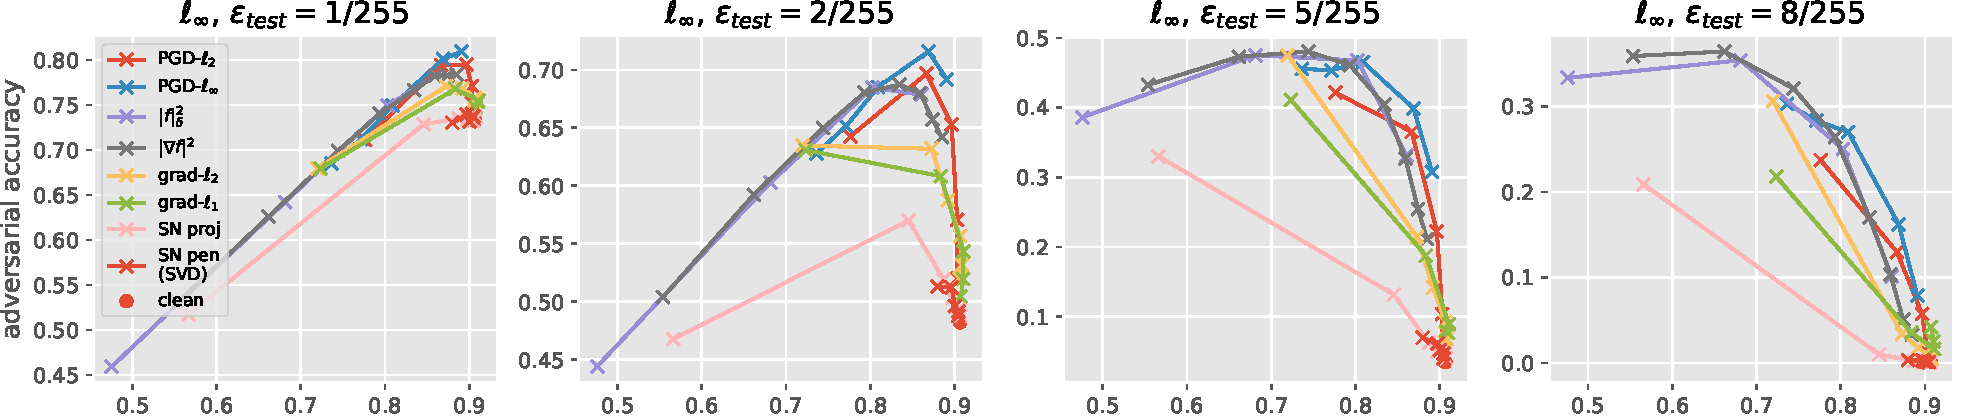
\includegraphics[width=.95\textwidth]{figures/cifar10_vgg/test_vs_adv_linf.pdf}
% 	\caption{$\ell_\infty$ robustness trade-off curves of different regularization methods for VGG11 on CIFAR10.
% 	Each plot shows test accuracy vs adversarial test accuracy
% 	for $\ell_\infty$ bounded 40-step PGD adversaries with a fixed~$\epsilon_{\text{test}}$.
% 	Different points on a curve correspond to training with different regularization strengths,
% 	with the leftmost points corresponding to the strongest regularization.}
% 	\label{fig:robust_tradeoffs_linf}
% \end{figure*}


\section{Details on Generalization Guarantees}
\label{sec:generalization_appx}
%!TEX root = main.tex

This section presents the proof of Proposition~\ref{prop:robust_margin_bound},
which relies on standard tools from statistical learning theory~\citep[\eg,][]{boucheron2005theory}.

\subsection{Proof of Proposition~\ref{prop:robust_margin_bound}}
\begin{proof}
Assume for now that~$\gamma$ is fixed in advance, and let $\mathcal F_\lambda := \{f \in \Hc : \|f\|_\Hc \leq \lambda\}$.
Note that for all~$f \in \mathcal F_\lambda$ we have
\begin{align*}
\text{err}_\mathcal{D}(f, \epsilon) = P(\exists \|\delta\| \leq \epsilon: y f(x + \delta) < 0) \leq P(yf(x) < \lambda \epsilon) =: L^{\lambda \epsilon}(f),
\end{align*}
since~$\|f\|_\Hc \leq \lambda$ is an upper bound on the Lipschitz constant of~$f$.
Consider the function
\begin{align*}
\phi(x) = \begin{cases}
	0, &\text{ if }x \leq -\gamma - \lambda \epsilon\\
	1, &\text{ if }x \geq - \lambda \epsilon\\
	1 + (x + \lambda \epsilon)/\gamma, &\text{ otherwise.}
\end{cases}
\end{align*}
Defining $A(f) = \E \phi(-y f(x)) \geq L^{\lambda \epsilon}(f)$ and $A_n(f) = \frac{1}{n} \sum_{i=1}^n \phi(- y_i f(x_i)) \leq L_n^{\lambda \epsilon + \gamma}(f)$,
and noting that $\phi$ is upper bounded by 1 and $1/\gamma$ Lipschitz,
we can apply similar arguments to~\citep[Theorem 4.1]{boucheron2005theory} to obtain,
with probability $1 - \delta$,
\begin{equation*}
L^\lambda \epsilon(f) \leq L_n^{\lambda \epsilon + \gamma}(f) + O \left(\frac{1}{\gamma} R_n(\mathcal{F}_\lambda) + \sqrt{\frac{\log 1/\delta}{n}} \right),
\end{equation*}
where~$R_n(\mathcal{F}_\lambda)$ denotes the empirical Rademacher complexity of~$\mathcal{F}_\lambda$ on the dataset $\{(x_i, y_i)\}_{i=1, \ldots, n}$.
Standard upper bounds on empirical Rademacher complexity of kernel classes with bounded RKHS norm yield the following bound
\begin{align*}
\text{err}_\mathcal{D}(f, \epsilon) \leq L_n^{\lambda \epsilon + \gamma}(f) + O \left( \frac{\lambda}{\gamma \sqrt{n}} \sqrt{\frac{1}{n}\sum_{i=1}^n K(x_i, x_i)} + \sqrt{\frac{\log 1/\delta}{n}} \right).
\end{align*}
Note that the bound is still valid with $\gamma' \geq \gamma$ instead of~$\gamma$ in the first term
of the r.h.s., since $L_n^{\gamma}(f)$ is non-decreasing as a function of~$\gamma$.

In order to establish the final bound, we instantiate the previous bound for values $\lambda_i = 2^i$ and $\gamma_j = 2^{-j}$.
Defining $\delta_{i,j} = \frac{\delta}{(1 + 4i^2) \cdot ( 1 + 4j^2)}$, we have that w.p. $1 - \delta_{i,j}$, for all $f \in \mathcal F_{\lambda_i}$ and all $\gamma \geq \gamma_j$,

\begin{align}
\label{eq:bound_single}
\text{err}_\mathcal{D}(f, \epsilon) \leq L_n^{\lambda_i \epsilon + \gamma}(f) + O \left( \frac{\lambda_i}{\gamma_j \sqrt{n}} \sqrt{\frac{1}{n}\sum_{i=1}^n K(x_i, x_i)} + \sqrt{\frac{\log 1/\delta_{i,j}}{n}} \right).
\end{align}
By a union bound, this event holds jointly for all integers $i, j$ w.p. greater than $1 - \delta$,
since $\sum_{i,j} \delta_{i,j} \leq \delta$.
Now consider an arbitrary $f \in \Hc$ and $\gamma > 0$ and let $i = \lceil \log_2 \|f\|_\Hc \rceil$
and $j = \lceil \log_2 (1/\gamma) \rceil$. We have
\begin{align*}
\lambda_i &\leq 2 \|f\|_\Hc \\
\frac{1}{\gamma_j} &\leq \frac{2}{\gamma} \\
\log(1/\delta_{i,j}) &\leq \log(C(\|f\|_\Hc, \gamma) / \delta),
\end{align*}
with $C(\|f\|_\Hc, \gamma) := (1 + 4(\log_2\|f\|_\Hc)^2) \cdot (1 + 4(\log_2 (1/\gamma))^2)$.
Applying this to the bound in~\eqref{eq:bound_single} yields the desired result.

\end{proof}


\end{document}
